%%%%%%%%%%%%%%%%%%%%%%%%%%%%%%%%%%%%%%%%%%%%%%%%%
%
%	MSc THESIS TEMPLATE
%	developed for my master thesis at the Universitá di Torino
%
%	by Eugenio Senes (eugenio.senes@gmail.com)
%
%	released under MIT license, so share, modify and enjoy, but quoting the author !
%
%%%%%%%%%%%%%%%%%%%%%%%%%%%%%%%%%%%%%%%%%%%%%%%%%

%% DOCUMENT CLASS (alternative to book is 'report')
% Print just right page or both sides (comment the other one)
\documentclass[12pt,a4paper,openright,oneside]{book}	%%One sided
%\documentclass[12pt,a4paper,openright,twoside]{book}	%%Double sided


%% SET MARGINS OF THE PAGES
\usepackage{geometry}
\geometry{a4paper,portrait, left=35mm, right=20mm, top=35mm, bottom=30mm}

\usepackage{textcomp,mathcomp}

%% HEADERS AND FOOTERS
\usepackage{fancyhdr}
\pagestyle{fancy}
\fancyhf{} 			%clears default header and footer
\rhead{} 			%right head
\lhead{ \leftmark} 	%left head
\rfoot{\thepage}
%%consider using also chead, cfoot, lfoot
%coherce the plain stile to this (e.g. the first page of every chapter)
\fancypagestyle{plain}{
	\fancyhf{}
	\rfoot{\thepage}
	\renewcommand{\headrulewidth}{0pt}
	\renewcommand{\footrulewidth}{0pt}
}
%% CLEAR PAGE WITHOUT NUMBER AT THE BEGINNING OF CHAPTERS
\let\origdoublepage\cleardoublepage
\newcommand{\clearemptydoublepage}{%
  \clearpage
  {\pagestyle{empty}\origdoublepage}%
}
%% ALLOW PAGE ROTATION
\usepackage{lscape}

%% HYPERTEXT SETUP
\usepackage{hyperref}
\hypersetup{
    colorlinks,
    citecolor=black,
    filecolor=black,
    linkcolor=black,
    urlcolor=black
}
%% PDF SETTINGS
\hypersetup{
    pdfauthor={AuthorName},
    pdftitle={shortTitle},
    pdfsubject={subject},
    pdfkeywords={keyword1, keyword2}
}
%% FONTS AND SYMBOLS
\usepackage[utf8]{inputenc}	%%input font setting
\usepackage[T1]{fontenc} 		%%font for automatic recognition of letters with the accent
\usepackage{amsfonts}		%%fonts for the mathematical rendering of formulas
\usepackage{amssymb}
\usepackage{amsmath}
%% CHAPTERS STRUCTURE
\usepackage[italian,english]{babel} %%Set English as main language of the document
%% FIGURES
\usepackage{graphicx}
\usepackage{subfigure}		%%allow side by side figures with single caption
%% TABLES
\usepackage{multirow}		%%allow to merge rows in the tables
\usepackage{booktabs}		%%allow use of \toprule, \midrule, \bottomrule in tables
%%CAPTIONS
\usepackage{caption}
%% BIBLIOGRAPHY
\usepackage[babel]{csquotes}
%% CODE LISTINGS
\usepackage{listings}		%%allow to use code listings

%% HYPENATON
\hyphenation{te-si pip-po paperino}	%manual hyphenation


%%%%%%%%%%%%%%%%%%%%%%%%%%%%%%%%%%%%%%%%%%%%%%%%%
%%%% BEGIN DOCUMENT
\begin{document}

%%%%%% HEAD  OF THE DOCUMENT
\frontmatter
%%FRONT PAGE
\begin{titlepage}
%upper part
\begin{center}
{{\Large{\textsc{Universit\`a degli studi di Torino \\}}}} \vspace{5mm} {\small{\bf SCUOLA DI SCIENZE DELLA NATURA\\ \vspace{3mm}
Corso di Laurea Magistrale in Informatica}}
\vspace{5mm}
\end{center}
%logo
\begin{center}

\includegraphics[scale=.3]{head/logo.png}
\end{center}
%title
\begin{center}
\vspace{5mm}
{\large{\bf Tesi di Laurea Magistrale\\}}
\vspace{5mm}
{\LARGE{\bf UNSUPERVISED ANOMALY DETECTION\\ PER UN INDUSTRIA MANUFATTURIERA\\}}
%\vspace{5mm}
%{\LARGE{\bf SECOND ROW TITLE}}
\end{center}
\vspace{20mm}
%relatore
\par
\noindent
\begin{minipage}[t]{0.47\textwidth}
\vspace{20mm}
{\large{\bf Relatore:}\\
Prof. Andras Horvath}
\end{minipage}
\hfill
\begin{minipage}[t]{0.47\textwidth}\raggedleft
\vspace{20mm}
{\large{\bf Candidato:}\\
Giraudo Loris}
\end{minipage}
\vspace{10mm}
\begin{center}
{\large{\bf 
Anno Accademico 2021/2022}}
\end{center}

\end{titlepage}
\clearemptydoublepage
%%DEDICATION (the initial quote)
\thispagestyle{empty}
\begin{flushright}

\vspace*{60mm}

A me stesso, ai miei familiari ed ai miei amici\\
per il sostegno in questo percorso.


\end{flushright}
%\clearemptydoublepage
%%ABSTRACT
\chapter*{Abstract}
L’Anomaly Detection è un topic sempre più importante e il suo utilizzo spazia dal campo medico per arrivare a quello finanziario passando anche per approcci più standard come l'analisi di sensori installati su strumenti o macchinari.

Il task che risolve è quello di identificare eventi od osservazioni rari oppure che deviano in maniera significativa dalla maggioranza dei dati e che non corrispondono a una definizione di comportamento normale. Ricercare queste anomalie può essere utile quando si devono applicare metodi statistici e una pulizia dei dati è necessaria, ma non solo. In molte applicazioni le anomalie sono di alto interesse in quanto possono contenere informazioni di rilievo e quindi necessitano di attenzione. 

I metodi di Anomaly Detection si dividono tra supervisionati, semi-supervisionati o non supervisionati e un ampio numero di essi sono stati proposti nella letteratura ma non esiste un metodo che sia il più accurato per ogni dataset. Inoltre, la disponibilità di etichette di anomalia per un certo dataset è solitamente bassa o completamente assente nella pratica. 


L’obiettivo di questa tesi è quello applicare metodi non supervisionati di Anomaly Detection all'interno del progetto Beat 4.0 portato avanti da SKF e ALTEN ITALIA. 

A seguito di un'introduzione sul contesto in cui si opera, dei problemi e delle principali tecniche proposte nella letteratura, verrà mostrato un algoritmo di Model Selection che va a rispondere alla seguente domanda: dato un dataset senza etichette e un set di Anomaly Detectors, come poter selezionare il modello più accurato? A questo scopo vengono definite tre classi di metriche non supervisionate chiamate \textit{Model Centrality}, \textit{Clustering Coefficient} e \textit{Performance on Injected Synthetic Anomalies} e viene mostrato come queste siano correlate rispetto alla metrica supervisionata F1-Score. Saranno proposti anche diversi metodi di Rank Aggregation: Borda, Robust Borda, AVG Score e Kemeny-Young utilizzati per combinare le tre metriche non supervisionate, e un'analisi approfondita sulle performance di ognuno rispetto a dataset di benchmark provenienti da ODDS e SMD.


\clearemptydoublepage
%%INDEXES
%summary
\tableofcontents
\clearemptydoublepage

%%%%%% BODY OF THE DOCUMENT
\mainmatter
%%INTRODUCTION
\chapter{Introduzione}
\label{chap:first-chapter-intro}
Il campo dell'Anomaly Detection sta ricevendo molto interesse nell'ultimo periodo. L'avanzamento tecnologico ha portato alla nascita dei Big Data e degli approcci Data Driven consentendo a tecniche di Machine Learning di spopolare in tantissimi ambiti, tra cui quello dell'industria 4.0.
Attraverso l'innovazione degli impianti di produzione e all'utilizzo di dispositivi IoT, gli operatori possono monitorare il comportamento di un canale di produzione e intervenire nel caso di anomalie oppure pianificare la produzione grazie all'analisi di dati statistici o report.
Solamente questo ha permesso un'evoluzione sostanziale ma non ci si ferma qui, l'enorme quantità di dati raccolti rende possibile l'applicazione di tecniche di Machine Learning come supporto alle scelte decisionali in diversi ambiti: Anomaly Detection, Predictive Maintenance, previsioni e molto altro.

L’obiettivo di questa tesi é quello di contribuire al progetto Beat 4.0 portato avanti da SKF e ALTEN ITALIA. SKF é una azienda multinazionale specializzata nella produzione di cuscinetti a sfera, ALTEN é un'azienda leader nel mercato europeo della consulenza informatica e che sta offrendo supporto ad SKF. Questa collaborazione ha lo scopo di portare innovazione digitale all'impianto SKF di Cassino in provincia di Frosinone, attraverso l'applicazione di tecniche di Machine Learning.
Diverse collaborazioni sono state concluse, mentre altre ancora in corso, tra ALTEN e l'Università degli Studi di Torino per portare avanti il progetto Beat 4.0. Ognuna di queste si focalizza in un dominio specifico del Condition Monitoring: previsione della qualità, studio di correlazione tra i sensori e la qualità finale, Predictive Maintenance ed infine Anomaly Detection su cui si basa il lavoro di questa tesi.
Il contributo dello studente si concentra su tutto il ciclo di vita di produzione di tecniche di Machine Learning: studio qualitativo e processamento dei dati, analisi e applicazione dei metodi di Anomaly Detection ed infine distribuzione degli algoritmi su Cloud Azure e sviluppo front-end attraverso PowerBI.
Il focus della tesi si é concentrato prevalentemente sullo studio e sull'applicazione di tecniche di Model Selection non supervisionato: la mancanza di etichette all'interno del dataset fornitoci da SKF non permette la valutazione di un modello di Anomaly Detection, costringendo quindi a ricercare metodi che non ne richiedessero l'uso. Solitamente il Model Selection si effettua andando a partizionare i dati in modo diverso per la fase di train-test, oppure facendo ottimizzazione degli iperparametri, ma in ogni caso la presenza di etichette é necessaria. Per questo motivo vengono introdotte due tecniche di Model Selection non supervisionate, chiamate Meta Learning e Metriche Surrogate. La prima richiede di allenare dei rilevatori di anomalie su dataset etichettati per poi trasferire le informazioni apprese ad un dataset non etichettato che sia sufficientemente simile al primo, quindi questo approccio é stato scartato. Il secondo si basa sulla creazione di metriche non supervisionate, chiamate surrogate, che siano sufficientemente correlate alle più classiche metriche supervisionate come F1-Score. Verranno quindi proposte tre metriche surrogate chiamate \textit{Model Centrality}, \textit{Clustering Coefficient} e \textit{Performance on Injected Synthetic Anomalies} insieme a diversi metodi di Rank Aggregation: Borda, Robust Borda, AVG Score e Kemedy-Young utilizzati per combinare insieme le 3 metriche non supervisionate.

Il proseguo della tesi si divide quindi in questo modo: i \textit{Capitoli \ref{chap:intro}}, \textit{\ref{chap:methods}} e \textit{\ref{chap:modelselection}} presentano un'introduzione dell'Anomaly Detection, metodi di Anomaly Detection e Thresholding, e Model Selection rispettivamente. Nel \textit{Capitolo \ref{chap:skf}} vengono trattati i dati SKF e le loro proprietà e caratteristiche. Il \textit{Capitolo \ref{chap:impl}} tratta tutta la fase di sperimentazione, con una prima parte dedicata all'implementazione delle metriche surrogate e di Rank Aggregation, una seconda parte contenente i risultati degli esperimenti su dataset di benchmark provenienti da ODDS e SMD ed infine una terza parte in cui viene testato l'algoritmo di Model Selection su SKF. Il \textit{Capitolo \ref{chap:deploy}} conclude il ciclo di vita del software andando a trattare la fase di pubblicazione su Cloud Azure.
Conclusione e sviluppi futuri sono invece trattati nel \textit{Capitolo \ref{chap:conclusion}}.
\clearemptydoublepage
%% CHAPTERS
\chapter{Anomaly detection}
\label{chap:intro}

\section{Definizione del problema}

L'Anomaly Detection, anche definita come Outlier Detection, è il processo di identificazione di eventi od osservazioni che hanno un comportamento anomalo. 
La definizione del termine anomalo è specifica al caso d'uso ma quella più comune va a definire l'anomalia come un'osservazione che devia in maniera significativa dalle altre.

Le anomalie nelle serie temporali sono punti o sequenze di punti che non corrispondono a un comportamento normale. Il concetto di comportamento normale è difficile da formalizzare, pertanto, un'altra possibile definizione di anomalie potrebbe essere un pattern di dati inaspettato mai stato visto prima.

Un presupposto implicito è che le anomalie siano eventi rari e non sono da confondere con il rumore presente nei dati. Il rumore è un fenomeno che, a differenza delle anomalie, ha meno interesse a essere analizzato.
Tuttavia, le anomalie possono indicare un problema significativo in diverse applicazioni. Ad esempio, un'anomalia nei sistemi di controllo industriale può indicare un malfunzionamento, anomalie finanziarie possono essere il risultato di una frode oppure nel campo medico possono indicare malattie o complicazioni.

\subsection{Tipi di anomalie}
Le anomalie possono essere classificate in tre categorie:
\begin{itemize}
	\item \textbf{Anomalie a Punto}: quando una singola osservazione devia significativamente dal resto dei dati.
	\item \textbf{Anomalie Contestuali}: quando una sequenza di punti è anomala rispettivamente al contesto in cui si trova ma è considerata normale rispetto ad altri contesti. Per esempio, una temperatura di 30 $\tccentigrade$ è normale in estate ma anomala in inverno. 
	\item \textbf{Anomalie Collettive}: quando una sequenza di punti è considerata anomala rispetto al resto dei dati, ma i punti presi singolarmente non lo sono.
\end{itemize}


\subsection{Applicazioni dell'anomaly detection}
L'Anomaly Detection può essere applicata in una vasta serie di domini, i quali possono presentare caratteristiche molto diverse tra loro. I più conosciuti sono:
\begin{itemize}
	\item \textbf{Finanziario}: in questo campo l'Anomaly Detection viene usata per rivelare una serie di acquisti o movimentazioni sospette, sia per quanto riguarda la frequenza, gli importi o la localizzazione.
	\item \textbf{Medico}: dati medici collezionati ad esempio da strumenti come ECG possono essere analizzati per scoprire anomalie che riflettono malattie.
	\item \textbf{Rilevamento di Intrusioni}: all'interno di sistemi informatici vengono raccolti diversi tipi di dati riguardanti chiamate di sistema, il traffico di rete o altre attività nel sistema. Questi dati possono mostrare un comportamento insolito a causa di attività sospette. Il rilevamento di tali attività è noto come rilevamento delle intrusioni di sistema.
	\item \textbf{Condition Monitoring}: i sensori sono spesso posti su strumenti o macchinari e scoprire pattern anomali può rivelare informazioni sulla salute o sul funzionamento degli impianti.
\end{itemize}

\subsection{Sfide}
Uno degli aspetti più complessi da tenere in considerazione quando si applicano tecniche di Anomaly Detection è quello di andare a definire un "comportamento normale" da usare come riferimento. Purtroppo, a volte riuscire a farlo è molto difficile per i seguenti motivi:
\begin{itemize}
	\item Le anomalie solitamente sono eventi rari, la cui frequenza è molto bassa. Di conseguenza i dati a disposizione possono essere molto pochi.
	\item Le anomalie possono avere una distribuzione di dati mai vista in precedenza, diventando così difficile distinguerle a priori.
	\item Le anomalie variano in base al contesto o dominio in cui si opera, rendendo impossibile la generalizzazione di un singolo metodo.
	\item Spesso non si hanno a disposizione etichette che identifichino anomalie all'interno di un dataset, oppure si ha solo una piccola porzione di etichette.
\end{itemize}
A causa di queste problematiche il rischio di avere molti falsi-positivi o falsi-negativi è alto. In questi casi è opportuno, tramite un trade-off, scegliere se preferire un numero di falsi allarmi più alto rispetto all'ignorare situazioni potenzialmente anomale.

\section{Serie temporali}
Una serie temporale è definita come una sequenza ordinata di valori, che rappresenta l'evoluzione di una variabile numerica nel tempo. È la misurazione di un sistema che evolve nel tempo con attributi numerici: ad esempio, la temperatura di un computer/server, il valore delle azioni di un'azienda o l'attività elettrica del cuore (ECG). Una serie temporale è, quindi, qualsiasi sequenza di osservazioni indicizzate dal tempo. Una serie temporale contiene molte informazioni sul sistema misurato e queste possono essere utilizzate per garantire il corretto funzionamento del sistema.

\subsection{Univariato e multivariato}
Una serie temporale univariata è un insieme di valori misurati che modellano e rappresentano il comportamento di un processo nel tempo. Invece, una serie temporale multivariata è un insieme di misurazioni correlate tra loro nel tempo, che modella e rappresenta il comportamento di un processo multivariato nel tempo. 

Più formalmente, una serie temporale univariata è una sequenza di punti
\[\tau = \left\{ x_1, \ldots, x_T  \right\}, x_i \in \mathbb{R}\]
ognuno dei quali è un'osservazione di un processo misurato in un momento specifico $t$. Le serie temporali univariate contengono una singola variabile in ogni istante di tempo, mentre le serie temporali multivariate registrano più di una variabile alla volta. Esse sono denotate da
\[\tau = \left\{ x_1, \ldots, x_T  \right\}, x_i \in \mathbb{R}^k \]

\subsection{Decomposizione delle serie temporali}
Una serie temporale è un'aggregazione di quattro componenti: trend, stagionalità, livello e rumore.

\subsubsection{Trend}
Il trend rappresenta l'evoluzione a lungo termine della serie temporale in esame. Rifletta il comportamento "generico" della serie.

\subsubsection{Stagionalità}
La stagionalità corrisponde ad un pattern che si ripete regolarmente nel tempo.

\subsubsection{Livello}
Il livello corrisponde al valore medio della serie temporale. Se questa ha trend, allora il livello cambierà.

\subsubsection{Rumore}
Il rumore corrisponde a fluttuazioni irregolari di natura casuale.

\subsection{Stazionarietà}
La caratteristica della stazionarietà è rappresentata dalla capacità di un processo di essere de-correlato da un indice temporale. Una serie temporale $T$ è detta stazionaria quando la distribuzione, e quindi anche il valore medio del processo, è indipendente da $t$. 

La stazionarietà indica stabilità dove la distribuzione di $\left\{ x_1, \ldots, x_T  \right\}$ è identica alla distribuzione $\left\{ x_2, \ldots, x_{T+1}  \right\}$ in cui la serie oscilla intorno alla media con una varianza costante.
\clearemptydoublepage
\chapter{Metodi di anomaly detection}
\label{chap:methods}

\section{Modelli di apprendimento}
I modelli di apprendimento sono algoritmi che utilizzano dati per apprendere come effettuare una determinata attività come la classificazione o la regressione. Ci sono diverse categorie di modelli di apprendimento, tra cui:
\begin{enumerate}
\item \textbf{Modelli supervisionati}: utilizzano dati etichettati (in cui la risposta corretta è nota) per apprendere in base alla loro etichetta.
\item \textbf{Modelli non supervisionati}: utilizzano dati non etichettati (in cui la risposta corretta non è nota) per scoprire relazioni e strutture all'interno dei dati.
\end{enumerate}

I modelli di apprendimento sono utilizzati in molte aree, tra cui il riconoscimento delle immagini, il processamento del linguaggio naturale, la previsione delle serie temporali, la robotica e molte altre.

\subsection{Modelli supervisionati}
I modelli di apprendimento supervisionato sono una categoria di algoritmi di apprendimento automatico che utilizzano dati etichettati per "imparare" come effettuare una determinata attività. Il processo di apprendimento consiste nell'allenare il modello su un insieme di dati di addestramento etichettati, in cui la risposta corretta è nota, e quindi testarlo su un insieme di dati di test per valutare le sue prestazioni. Quando il modello riceve un nuovo dato da predire lo compara rispetto ciò che ha appreso durante la fase di allenamento. I principali task dei modelli supervisionati sono due: classificazione e regressione.

\subsubsection{Classificazione}
La classificazione è il problema di identificare a quale categoria o classe un'osservazione appartiene. Un classificatore, definito come \(\hat{c}\), è una funzione che mappa uno spazio di input \(X\), che definisce come i dati sono descritti, ad uno spazio di output \(C=\{C_1,...,C_k\}\) ovvero il set finito di etichette
\[\hat{c}: X \rightarrow C\]
Nel campo dell'apprendimento supervisionato gli esempi sono accompagnati da delle etichette e sono dunque definiti come \((x,c(x))\in X\times C\) dove \(x \in X\) e \(c(x)\) è la corretta classe di \(x\). Il task di classificazione è quello di andare a costruire la funzione \(\hat{c}\) che meglio approssima la funzione reale \(c\) non solo nei dati di training ma nell'intero spazio \(X\). Questa è una condizione importante perché vogliamo che il classificatore generalizzi bene e non faccia over-fitting. Over-fitting si ha quando un classificatore ha performance molto alte sui dati di training ma molto basse sui dati di test.
Esistono 4 tipi di classificatori:
\begin{enumerate}
\item \textbf{Classificatori binari}: è il più semplice in quanto l'insieme delle classi contiene solo due elementi: \(C=\{C_1,C_2\}\).
\item \textbf{Classificatori a score}: sono delle funzioni che assegnano uno score alla predizione: \(\hat{s} = X\rightarrow R^k\) dove \(X\) rappresenta lo spazio di input mentre l'output è definito da un vettore di \(k\) numeri reali: 
\[(\hat{s}_1 (x),...,\hat{s}_k(x))\]
In questo vettore, il componente k-esimo è lo score assegnato alla classe \(C_k\) per l'istanza \(x\). Generalizzando, per ogni istanza \(x\) esiste un vettore \(\hat{s}(x)\) contenente i punteggi \(\hat{s}_k(x)\) per ogni classe \(k\) di \(C\).
\item \textbf{Classificatori probabilistici}: eredita delle caratteristiche dai classificatori a score con la differenza che il valore di ogni componente del vettore di output di una istanza \(x\) rappresenta la probabilità che quell'istanza ricada nella classe \(k\). Essendo probabilità, la somma totale di tutti i valori all'interno del vettore corrisponde a 1.
\item \textbf{Classificatori multiclasse}: sono un'estensione dei classificatori binari con un insieme delle classi maggiore di due elementi: \(C=\{C_1,...,C_k\}\). 
\end{enumerate}

\subsubsection{Regressione}
All'interno del task di regressione siamo di fronte non più ad un codominio finito, come nel caso della classificazione, ma un codominio rappresentato dall'insieme dei numeri reali \(R\). I modelli di regressione sono quindi definiti da una funzione
\[\hat{f}: X \rightarrow \mathbb{R}\]
Il problema di apprendimento è anche qui quello di trovare la funzione \(\hat{f}\) che meglio approssima la funzione reale \(f: (x_i, f(x_i))\) per ogni \(x\in X\).
Cambiando l'obiettivo della funzione da un numero relativamente piccolo di classi a uno spazio di soluzioni infinito, l'algoritmo cercherà di stimare i valori associati a ciascun esempio nel modo più accurato possibile, il che porterà al problema dell'overfitting. Tenendo presente che è necessario accettare un equilibrio tra accuratezza e approssimazione delle soluzioni, è inevitabile, di fronte alle normali oscillazioni dei dati, che il modello non possa catturarle con precisione. Il vero scopo di un modello di regressione è quello di approssimare l'andamento della funzione $f$ nel miglior modo possibile. La Figura \ref{overfitting} mostra un esempio di problema di regressione: la linea rossa rappresenta una funzione che fa overfitting, ovvero è precisa sui dati di training. Questo comporta un basso livello di bias ma alta varianza: i dati nuovi non riuscirà a predirli con precisione. Le linee blu invece rappresentano modelli più "semplici" che generalizzano meglio, hanno quindi un bias più alto ed una varianza più bassa.

\begin{figure}[t]
	\centering
	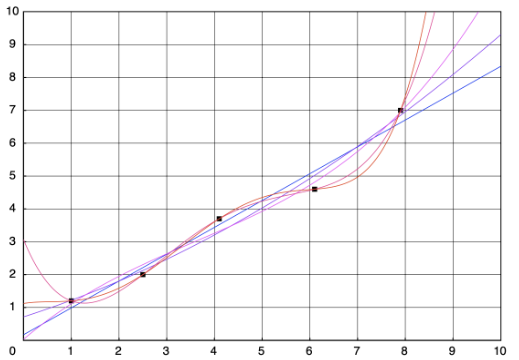
\includegraphics[width=10cm, scale=1]{images/overfitting}
	\caption{Overfitting}
	\label{overfitting}
\end{figure}


\subsection{Modelli non supervisionati}
L'apprendimento non supervisionato è una categoria di algoritmi di apprendimento automatico che utilizzano dati non etichettati per "imparare" da essi. In contrasto con l'apprendimento supervisionato, dove ci sono dati etichettati con le risposte corrette, l'apprendimento non supervisionato non ha accesso alle risposte corrette, ma cerca di scoprire relazioni o strutture all'interno dei dati.

Ci sono diverse tipologie di algoritmi di apprendimento non supervisionato, tra cui:
\begin{itemize}
\item \textit{Clustering}: utilizzato per raggruppare gli esempi in base alle loro similitudini.
\item \textit{Riduzione della dimensionalità}: utilizzato per ridurre la dimensionalità dei dati.
\item \textit{Analisi di componenti principali (PCA)}: utilizzato per individuare le componenti principali dei dati.
\item \textit{Anomaly Detection}: utilizzato per identificare dati anomali o fuori dalla norma.
\item \textit{Modelli Generativi}: utilizzati per generare nuovi dati.


\end{itemize}
Nel rilevamento supervisionato delle anomalie, se vogliamo che un modello sia in grado di rilevare le anomalie, bisogna allenare il sistema in modo molto preciso sia nell'identificare il comportamento normale che quello anomalo.
Tuttavia, i comportamenti normali possono essere molteplici così come i
comportamenti in presenza di anomalie e questo porta con se la necessità di fornire una grande quantità di dati etichettati per catturare più comportamenti possibili. Purtroppo non è sempre possibile in quanto le anomalie sono eventi rari e se il dataset di addestramento è relativamente piccolo, anche il numero di anomalie non sarà sufficientemente grande, rendendo difficile la loro classificazione. 
Pertanto, l'apprendimento non supervisionato si adatta perfettamente al problema del rilevamento delle anomalie, poiché non è necessario etichettare i dati. Inoltre, una parte delle anomalie derivano da nuovi comportamenti del sistema e per definizione questi comportamenti non possono essere classificati correttamente con i metodi di rilevamento delle anomalie supervisionati senza effettuare prima un re-training.


\section{Valutazione del modello}
La valutazione del modello è necessaria per quantificarne le prestazioni. La
scelta delle metriche e delle tecniche di valutazione dipende dal task di apprendimento come la classificazione o la regressione. 
In questa sezione ci si concentrerà sulle tecniche e sulle metriche più famose utilizzate per valutare la performance di un modello su un determinato compito.

\subsubsection{Tecniche}
\begin{itemize}
	\item \textbf{Random Split} genera in maniera casuale i tre insiemi di train, test e validazione. Il vantaggio di questo metodo è che c'è una buona probabilità che la popolazione originale sia ben rappresentata in tutti e tre gli insiemi, impedendo quindi un campionamento distorto dei dati.
	\item \textbf{Time Based Split} viene applicato sulle serie temporali in cui non è possibile effettuare una suddivisione casuale dei dati in quanto si andrebbe a perdere informazioni come trend o stagionalità. 
	      In questi casi, si utilizza una suddivisione temporale in cui, ad esempio, l'insieme di train può contenere i dati più vecchi, mentre quelli più recenti sono assegnati all'insieme di test. Per evitare l'overfitting introdotto da questo metodo, una variante a finestre di scorrimento è preferibile: il modello viene allenato iterativamente più volte su una finestra temporale e valutato sulla parte restante dei dati, per poi allargare la finestra di training ad ogni iterazione (riducendo così quella di valutazione).
	\item \textbf{K-Fold Cross Validation} tiene in considerazione due tipologie di dati: il test set ed il train set. Per formare questi insiemi, genera in modo casuale $k$ gruppi di dati ed iterativamente vengono usati $k-1$ gruppi per il training ed un gruppo per il test.
	\item \textbf{Stratified K-Fold} è simile al Cross Validation ma con la differenza che questo metodo tiene in considerazione la distribuzione delle classi dei dati, generando quindi gruppi con rateo simile al dataset originale.
\end{itemize}


\subsubsection{Metriche}
Alla base di tutte le metriche di valutazione vi è la tabella di contingenza. Questa tabella permette di valutare le performance di un modello andando a relazionare, in più modi, le predizioni di un modello con le etichette reali.

La Tabella \ref{contigency-table} mostra la struttura della tabella di contingenza.  La prima colonna contiene il numero delle predizioni positive fatte da un modello divise se queste sono effettivamente positive o negative. La seconda colonna funziona allo stesso modo ma per le predizioni negative. La terza colonna invece rappresenta la somma dei punti che sono realmente positivi e realmente negativi.
Riassumendo:
\begin{itemize}
\item \textit{True Positive}: punti realmente positivi che sono predetti come tali.
\item \textit{False Positive}: punti realmente positivi ma predetti come negativi.
\item \textit{False Negative}: punti realmente negativi ma predetti come positivi.
\item \textit{True Negative}: punti realmente negativi che sono predetti come tali.
\item \textit{Pos}: Somma totale dei punti realmente positivi.
\item \textit{Neg}: Somma totale dei punti realmente negativi.
\end{itemize}

\begin{table}[]
\centering
	\caption{\label{contigency-table}Tabella di contingenza}

\begin{tabular}{|l|l|l|l|}
\hline
                 & \textbf{Predizioni +} & \textbf{Predizioni -} & \textbf{Totale} \\ \hline
\textbf{Reale +} & TP                    & FN                    & Positivi        \\ \hline
\textbf{Reale -} & FP                    & TN                    & Negativi        \\ \hline
\end{tabular}
\end{table}

Definiamo prima $T_e$ come l'insieme dei punti del nostro dataset, a questo punto è possibile introdurre tutte le misure di performance:
\begin{itemize}
\item \textit{Accuracy}: è il rapporto tra i punti correttamente classificati rispetto al totale dei punti.
\[\frac{1}{|T_e|} \sum_{x \in T_e} I[\hat{c}(x)=c(x)]\]
\item \textit{Error Rate}: è il rapporto tra i punti erroneamente classificati rispetto al totale dei punti, in breve \(1-accuracy\).
\[\frac{1}{|T_e|} \sum_{x \in T_e} I[\hat{c}(x)\neq c(x)]\]
\item \textit{True Negative Rate / Specificity}: è il rapporto tra i punti classificati correttamente come negativi rispetto al numero totale di punti realmente negativi.
\[\frac{\sum_{x \in T_e} I[\hat{c}(x)=c(x)=-]}{\sum_{x \in T_e} I[c(x)=-]}\]
\item \textit{True Positive Rate / Recall}: è il rapporto tra i punti classificati correttamente come positivi rispetto al numero totale di punti realmente positivi.
\[\frac{\sum_{x \in T_e} I[\hat{c}(x)=c(x)=+]}{\sum_{x \in T_e} I[c(x)=+]}\]
\item \textit{Precision}: è il rapporto tra i punti correttamente classificati come positivi rispetto al numero di punti classificati come positivi.
\[\frac{\sum_{x \in T_e} I[\hat{c}(x)=c(x)=+]}{\sum_{x \in T_e} I[\hat{c}(x)=+]}\]
\item \textit{F-Measure Score}: è la media armonica tra precision e recall.
\[F_\beta=\frac{\left(1+\beta^2\right) \cdot(\text { precision } \cdot \text { recall })}{\left(\beta^2 \cdot \text { precision }+\text { recall }\right)}\]
\end{itemize}
Quest'ultima misura introduce il parametro $\beta$ che serve per dare più o meno peso alle componenti della formula: se $\beta = 1$, allora sia la precision che la recall avranno lo stesso peso, un valore di $\beta < 1$ da più peso alla precision, infine un valore di $\beta > 1$ da più peso alla recall.

In generale non esiste una misura migliore e bisogna fare un'attenta valutazione su quale sia la preferibile rispetto al task da risolvere.
Ad esempio bisogna tenere in considerazione se c'è una prevalenza di punti di una classe. Accuracy è preferibile quando ci si aspetta una distribuzione equa delle classi. Quando i falsi-negativi non sono di interesse, ma lo sono i falsi-positivi, precision è preferibile; al contrario quando i falsi-negativi sono molto importanti e non ci interessa dei falsi-positivi, recall è la scelta corretta.
F-Measure invece è necessaria quando si cerca un bilanciamento tra precision e recall dando importanza a entrambi i falsi-positivi ed i falsi-negativi. 
All'interno del contesto SKF e Anomaly Detection le anomalie sono sicuramente importanti da riconoscere e marcarle come negative, quindi falsi-negativi, potrebbe risultare in problemi alla linea di produzione. Ma allo stesso tempo un modello che produce molti più positivi di quanto deve risulterebbe in una perdita di fiducia da parte dell'operatore che inizierebbe semplicemente ad ignorare il feedback del modello. Per questo motivo la scelta della metrica di valutazione è ricaduta sulla F-Measure.



\section{Modelli di apprendimento automatico}
In questa sezione vengono proposti diversi algoritmi e metodi di apprendimento automatico per l'Anomaly Detection, raggruppati per categoria.
I seguenti algoritmi sono implementati all'interno della libreria pubblica PyOD\footnote{Python Outlier Detection (PyOD): https://github.com/
yzhao062/pyod} e TODS\footnote{Automated Time-series Outlier Detection System
 (TODS): https://github.com/datamllab/tods} ed utilizzati nel processo di Model Selection discusso nei capitoli successivi.

\subsection{Modelli lineari}
I modelli lineari sono un tipo di algoritmo di Machine Learning utilizzato per fare previsioni. Essi rappresentano la relazione tra le variabili indipendenti (chiamate anche feature) e la variabile dipendente (chiamata anche obiettivo) con una equazione lineare. La forma generale di un modello lineare è: 
\[ Y = B_0 + B_1X_1 + B_2X_2 + ... + B_n \cdot X_n\]
dove $ Y $ è la variabile dipendente,  \(X_1, X_2, ..., X_n\)  sono le variabili indipendenti mentre \( B_0, B_1, B_2, ..., B_n\) sono i coefficienti del modello che vengono "appresi" dai dati.

\subsubsection{PCA}
La PCA \cite{shyu2003novel} è una riduzione lineare della dimensionalità che utilizza la Singular Value Decomposition dei dati per proiettarli in uno spazio dimensionale inferiore. Si tratta di spiegare la struttura di varianza-covarianza di una serie di variabili attraverso alcune nuove variabili che sono funzioni di quelle originali. Le componenti principali sono particolari combinazioni lineari delle \textit{p} variabili casuali  \(X_1, X_2, ..., X_p\) con tre importanti proprietà: (1) le componenti principali non sono correlate, (2) la prima componente principale ha la varianza più elevata, la seconda componente principale ha la seconda varianza più elevata e così via, e (3) la variazione totale in tutte le componenti principali combinate è uguale alla variazione totale delle variabili originali \(X_1, X_2, ..., X_p\). 
Queste componenti principali sono ricavabili da un'analisi degli autovalori della matrice di covarianza o della matrice di correlazione di \(X_1, X_2, ..., X_p\).
In questa procedura, la matrice di covarianza dei dati può essere decomposta in vettori ortogonali, detti autovettori, associati ad autovalori. Gli autovettori con alti autovalori catturano la maggior parte della varianza dei dati. Pertanto, un iperpiano a bassa dimensionalità costruito da \textit{k} autovettori può catturare la maggior parte della varianza dei dati. Tuttavia, gli outlier sono diversi dai punti di dati normali, cosa che è più evidente sull'iperpiano costruito dagli autovettori con autovalori piccoli.
Di conseguenza, i punteggi degli outlier possono essere ottenuti come la somma della distanza proiettata di un campione su tutti gli autovalori.

\subsubsection{K-PCA}
Kernel-PCA \cite{hoffmann2007kernel} è un'estensione non lineare di PCA. I dati di input sono mappati in uno spazio infinitesimale da cui K-PCA estrae le componenti principali. I tipi di kernel usati possono essere: lineare, polinomiale, sigmoidale o radiale.



\subsubsection{Auto-Regressivo}
In un modello a regressione multipla viene fatta previsione di una variabile di interesse attraverso una combinazione lineare di predittori. Un modello Auto Regressivo, invece, fa previsione di questa variabile di interesse usando una combinazione lineare su \textit{valori passati} di questa variabile. Il termine auto-regressione indica una regressione della variabile fatta su se stessa.
Di conseguenza, un modello auto-regressivo di ordine \textit{p} può essere scritto come:
\[y_t=c+\phi_1 y_{t-1}+\phi_2 y_{t-2}+\cdots+\phi_p y_{t-p}+\varepsilon_t\]
dove $\varepsilon_t$ è rumore bianco. Può essere visto come una regressione multipla ma con valori ritardati di $y_t$ come predittori. 
La deviazione di un valore predetto rispetto a quello reale viene usato come outlier score.

\subsubsection{MCD}
Minimum Covariance Determinant (MCD) \cite{rousseeuw1999fast, hardin2004outlier} è un metodo per stimare la media e la matrice di covarianza andando a minimizzare l'influenza delle anomalie. L'idea alla base è quella di stimare questi valori andando a selezionare un sottoinsieme dei dati nella quale le anomalie o sono completamente assenti o sono il meno possibile.
Immaginando un approccio brute-force, l'algoritmo itera su ogni possibile sottoinsieme dei dati di una dimensione specifica. Vengono poi stimati la media e la matrice di covarianza per ogni sottoinsieme e poi vengono mantenuti soltanto i valori per il sottoinsieme che ha il determinante della matrice di covarianza più piccolo. Il motivo di questo è perché il determinante di una matrice di covarianza indica quanto è larga una distribuzione. Di conseguenza MCD cerca di minimizzare questo andando a prendere la distribuzione più compatta. Questo consente di escludere le anomalie che saranno situate lontane dal resto dei dati.

\subsubsection{LMDD}
Linear Method for Deviation-based Outlier Detection (LMDD) \cite{arning1996linear} impiega il concetto di Smoothing Factor il quale indica quanto può essere ridotta la misura di dissimilarità andando a rimuovere un sottoinsieme degli elementi dal dataset. La funzione di dissimilarità può essere qualsiasi misura di dispersione come la varianza, inter-quantile range, mediana ecc.
I punti rimossi che riducono maggiormente questa misura di dissimilarità possono essere valutati come anomalie.

\subsection{Modelli non lineari}
I modelli non lineari riescono a modellare relazioni non lineari nei dati, catturando relazioni più complesse e anche non linearmente separabili, limite dei modelli lineari.

\subsubsection{OCSVM}
Il metodo One Class Support Vector Machine (OCSVM) \cite{scholkopf2001estimating} è una versione derivata dalle Support Vector Machine al rilevamento di una sola classe. L'idea alla base consiste nel minimizzare l'ipersfera contenente i punti di una singola classe e considerare tutti i punti esterni alla sfera come outliers.
La Figura \ref{ocsvm} mostra un esempio del funzionamento di OCSVM.
\begin{figure}[t]
	\centering
	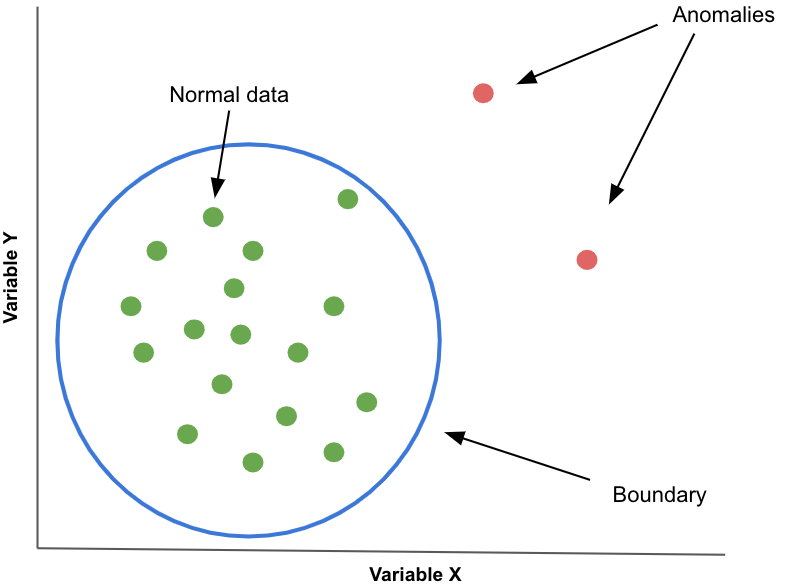
\includegraphics[width=8cm, scale=1]{images/ocsvm}
	\caption{OCSVM}
	\label{ocsvm}
\end{figure}

\subsection{Modelli a distanza}
I modelli non supervisionati basati sulla distanza sono una categoria di algoritmi che utilizzano la distanza tra i dati per scoprire relazioni e strutture nel dataset.

\subsubsection{KNN}
K-Nearest Neighbors (KNN) \cite{ramaswamy2000efficient,angiulli2002fast} è un algoritmo di apprendimento utilizzato per classificare oggetti in base alle loro proprietà. Dato un nuovo punto, l'algoritmo cerca i \textit{k} punti più simili (detti "vicini") tra quelli già classificati e assegna all'oggetto in esame la classe più comune tra i \textit{k} vicini trovati. La scelta del valore di \textit{k} è importante e può influire sulla sua accuratezza. In generale, un valore più alto di \textit{k} tende a ridurre la varianza del modello ma aumenta la sua bias.
Nel campo dell'Anomaly Detection non è di interesse assegnare la classe al punto in esame ma assegnare un punteggio di anomalia. Per un'osservazione, quindi, la sua distanza rispetto al \textit{k}-esimo punto più vicino rappresenta questo score.

\subsubsection{DBSCAN}
DBSCAN è un metodo di clustering che raggruppa i punti in aree ad alta densità e contrassegna i punti in regioni a bassa densità come anomali.
DBSCAN classifica quindi i punti in tre categorie. I punti centrali sono punti
contenenti almeno $minPts$ nel loro intorno definito da un parametro $\epsilon$. I border-point sono i punti che contengono almeno un punto centrale nel loro intorno, mentre gli altri punti sono considerati come rumore/anomalie. 


\subsubsection{LOF}
Local Outlier Factor (LOF) \cite{breunig2000lof} misura la deviazione locale di un dato punto rispetto ai suoi vicini. Sulla base del metodo dei KNN, la densità locale di questo punto viene valutata considerando la distanza rispetto ai suoi \textit{k} punti più vicini. Il punteggio di anomalia viene invece calcolato confrontando la sua densità locale con quella dei suoi \textit{k} vicini più prossimi. Un punteggio elevato indica una densità inferiore a quella dei suoi vicini e quindi potenzialmente un'anomalia. In Figura \ref{lof} è presente il funzionamento di LOF dove si possono notare cerchi più grandi per i punti più isolati.
\begin{figure}[t]
	\centering
	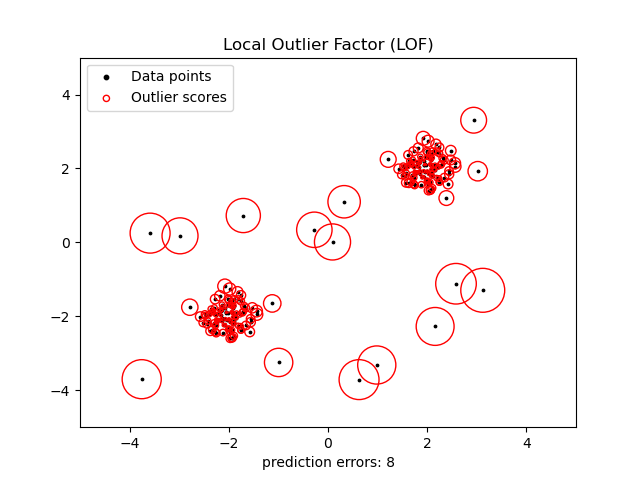
\includegraphics[width=10cm, scale=1]{images/lof}
	\caption{LOF}
	\label{lof}
\end{figure}

\subsubsection{COF}
Connectivity Outlier Factor (COF) \cite{tang2002enhancing} è un'evoluzione di LOF. Si basa sull'idea di assegnare un grado di anomalia ad ognuno dei punti, chiamato connectivity outlier factor.
Per ogni punto $x_i$, vengono selezionati i \textit{k} punti più vicini e viene generato il percorso minimo che attraversi tutti i \textit{k} punti partendo da $x_i$. Infine COF viene calcolato andando a fare una media delle distanze di ogni percorso di $x_i$ verso i suoi \textit{k} punti più vicini.

\subsubsection{CBLOF}
Cluster-Based Local Outlier Factor (CBLOF) \cite{he2003discovering} è anch'esso un evoluzione di LOF.
Come primo step, CBLOF riceve in input i dati ed un algoritmo di clustering per andare a formare dei cluster. Attraverso dei parametri va poi a definire quale cluster viene considerato "grande" e quale viene considerato "piccolo". Vengono poi calcolati gli outlier score per tutti i punti andando a considerare la dimensione del cluster a cui un punto appartiene e la distanza più vicina rispetto al centro di un cluster grande. Quindi più un cluster di appartenenza è piccolo e più il punto è lontano dal centro di un cluster grande, più lo score di anomalia sarà alto. 

\subsubsection{HBOS}
Histogram based outlier detection (HBOS) \cite{goldstein2012histogram} è un algoritmo di outlier detection che si basa sugli istogrammi assumendo indipendenza tra le features. Per ogni feature computa il rispettivo istogramma. Successivamente itera su ogni punto: se il valore di una feature di uno specifico punto $x_i$ rientra nella coda dell'istogramma, questo punto vede alzarsi lo score di anomalia. Questo passaggio viene ripetuto rispetto ad ogni feature e su tutti i punti.

\subsubsection{SOD}
Subspace outlier detection (SOD) \cite{kriegel2009outlier} cerca di trovare gli outlier andando a considerare diversi sottoinsiemi dello spazio multidimensionale delle feature. Per ogni osservazione, SOD esplora il sottoinsieme delle dimensioni che si dirama parallelamente dai punti vicini e determina quanto questa osservazione devia dai suoi vicini in questo sotto-spazio. 

\subsubsection{ROD}
Rotation-based Outlier Detection (ROD) \cite{almardeny2020novel},  è un algoritmo privo di parametri che non richiede conoscenza sulla distribuzione dei dati e funziona in modo intuitivo nello spazio tridimensionale, dove i vettori 3D, che rappresentano i punti, vengono ruotati attorno alla mediana geometrica due volte in senso antiorario utilizzando la formula di rotazione di Rodrigues. I risultati della rotazione sono parallelepipedi i cui volumi vengono analizzati matematicamente come funzioni di costo e utilizzati per calcolare le Deviazioni Assolute Mediane e ottenere così il punteggio di anomalia. Per dimensioni elevate > 3, il punteggio complessivo viene calcolato prendendo la media dei punteggi complessivi dei sottospazi 3D risultanti dalla scomposizione dello spazio dei dati originali.


\subsection{Modelli probabilistici}
I modelli probabilistici non supervisionati sono una categoria di algoritmi che utilizzano la probabilità per descrivere e generare i dati. Essi utilizzano una distribuzione di probabilità per rappresentare la relazione tra le variabili del dataset.
\subsubsection{KDE}
Kernel Density Estimation (KDE) \cite{latecki2007outlier} è l'applicazione di un "kernel smoothing" per la stima della probabilità. 
Siano $(x_1,...,x_n)$ osservazioni indipendenti e identicamente distribuite prese da una distribuzione univariata con una densità non conosciuta \textit{f} per qualsiasi punto \textit{x}. Siamo interessati nello stimare la forma di questa funzione \textit{f}. La funzione kernel di stima è:
\[\widehat{f}_h(x)=\frac{1}{n} \sum_{i=1}^n K_h\left(x-x_i\right)=\frac{1}{n h} \sum_{i=1}^n K\left(\frac{x-x_i}{h}\right)\]

Dove \textit{K} è il kernel, una funzione non negativa, e $h>0$ è un parametro di smoothing chiamato bandwidth. Un kernel con pedice $h$ è chiamato \textit{kernel scalato} ed è definito da: $Kh(x) = 1/h K(x/h)$. 
Il valore di $k$ deve essere scelto tenendo conto del trade-off bias/varianza.
I kernel più utilizzati sono: uniforme, triangolare e normale.
Le stime di densità con kernel sono fortemente correlate agli istogrammi, ma sono dotati di proprietà di smoothing o di valori continui usando appunto questi kernel.
La Figura \ref{kde_model} mostra un confronto tra un istogramma con una funzione di stima di densità con kernel.
L'applicazione di questo modello nell'Anomaly Detection avviene andando a generare, per un'osservazione, uno score di anomalia corrispondente al valore negativo del logaritmo della probabilità di densità.

\begin{figure}[t]
	\centering
	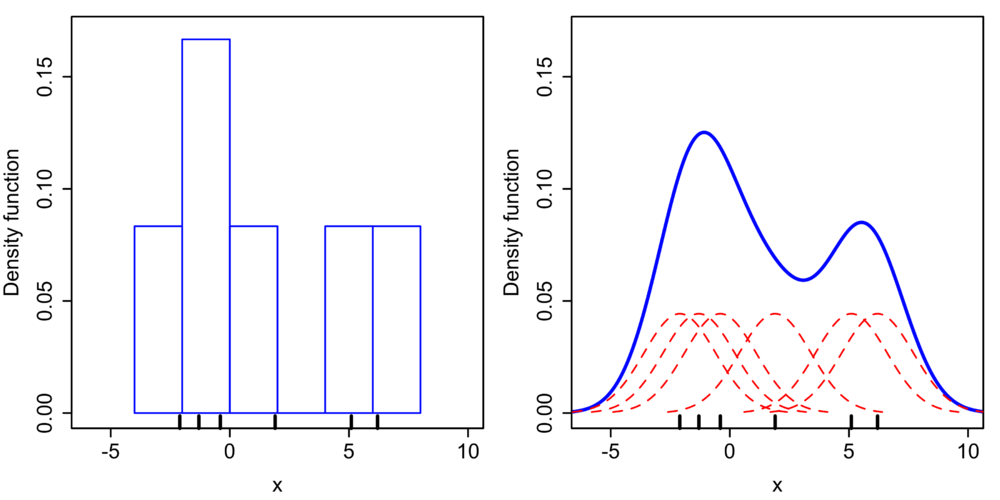
\includegraphics[width=10cm, scale=1]{images/kde_model}
	\caption{KDE}
	\label{kde_model}
\end{figure}


\subsubsection{GMM}
I GMM \cite{aggarwal2015outlier} sono una generalizzazione delle distribuzioni gaussiane e possono essere utilizzati per rappresentare qualsiasi serie di dati che possono essere raggruppati in più distribuzioni gaussiane. GMM è un modello probabilistico che presuppone che tutti i punti dati siano generati da una insieme di distribuzioni gaussiane con parametri sconosciuti e può essere utilizzato per il clustering, oppure per stimare la probabilità che un nuovo punto dati appartenga a ciascun cluster. Può essere inteso come un modello probabilistico in cui si ipotizzano distribuzioni gaussiane per ciascun gruppo, con medie e covarianze che ne definiscono i parametri.

Per la stima di questi parametri si esegue l'algoritmo di Expectation-Maximization chiamato così in quanto vengono alternate iterativamente due fasi: quella di expectation e quella di maximization. L'algoritmo parte inizializzando prima i parametri del GMM. A ogni iterazione, la fase di expectation calcola il valore atteso della funzione log-likelihood rispetto ai parametri correnti. Questa valore viene poi utilizzato per massimizzare la log-likelihood nella fase di massimizzazione.

È possibile adottare questo modello nell'Anomaly Detection allenandolo rispetto ad un set di dati e poi assegnando un punteggio ai nuovi punti: quelli significativamente diversi dal resto dei dati verranno marcati come anomalia.

\subsubsection{ABOD}
Angle Based Outlier Detection (ABOD) \cite{kriegel2008angle} si basa sull'idea di osservare l'angolo formato da un insieme di tre punti qualsiasi nello spazio delle feature multivariate. La varianza dell'ampiezza dell'apertura angolare risulta diversa per i punti anomali e per quelli normali: la varianza osservata è più alta per i punti inlier e più bassa per gli outlier, quindi tale misura può essere usata per separare punti normali da anomalie. ABOD funziona abbastanza bene nello spazio ad alta dimensionalità, a differenza di altre misure basate sulla distanza che soffrono della "curse of dimensionality" in quanto gli angoli possono fornire una rappresentazione migliore della vicinanza.
\begin{figure}[t]
	\centering
	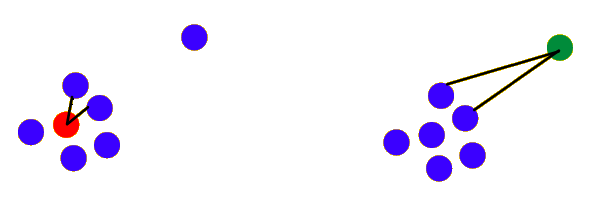
\includegraphics[width=10cm, scale=1]{images/abod}
	\caption{ABOD}
	\label{abod}
\end{figure}
Un esempio sull'idea alla base di ABOD è presente in Figura \ref{abod}.
Considerando il punto rosso come pivot, viene calcolato l'angolo racchiuso tra questo punto e qualsiasi altro punto dello spazio e con molta probabilità si noterà un'alta varianza tra questi valori. Questo andamento indica che il punto pivot fa parte di un cluster ad alta coesione.
Se si considera come pivot invece il punto verde e procedendo con gli stessi calcoli per ogni coppia di punti, la varianza angolare sarà molto più bassa, indice che quel punto è molto probabilmente un outlier.

\subsubsection{ECOD}
Empirical-Cumulative-distribution-based Outlier Detection (ECOD) \cite{li2021ecod} è un modello probabilistico che basa il suo funzionamento nel calcolare, per ogni punto $x_i \in X$, la probabilità che esista un punto almeno "estremo" come $x_i$.
ECOD prima stima la distribuzione dei dati di input senza l'ausilio di parametri esterni andando a computare la distribuzione cumulativa empirica per ogni dimensione del dataset. Successivamente usa la distribuzione empirica per stimare la probabilità, su ogni dimensione, per ogni punto. Infine computa lo score di anomalia di ognuno dei punti andando ad aggregare le stime di probabilità su tutte le dimensioni.

\subsubsection{COPOD}
Copula Based Outlier Detection (COPOD) \cite{li2020copod} si ispira alla copula per modellare la distribuzione dei dati multivariati. Costruisce dapprima una copula empirica e la utilizza per predire la tail-probability di ogni punto per determinare il suo
livello di "estremità". Intuitivamente, si può pensare a questo come a calcolare
un valore p-anomalo.

\subsubsection{SOS}
Stochastic Outlier Selection (SOS) \cite{janssens2012stochastic} utilizza il concetto di affinità per quantificare la relazione tra un punto e un altro. L'affinità è proporzionale alla somiglianza tra due punti di dati. Quindi un punto ha poca affinità con un punto dati dissimile. 
Un'osservazione viene classificata come outlier quando tutti gli altri punti hanno un'affinità insufficiente con esso.

\subsubsection{Sampling}
Sampling \cite{sugiyama2013rapid} è un algoritmo che cerca di approssimare, a favore di un tempo computazionale decisamente minore, KNN. Al posto di calcolare la distanza di un punto rispetto a tutti gli altri e prendere i \textit{k} più vicini, esegue prima una fase di sampling in cui estrae casualmente un sottoinsieme di punti per poi andare ad effettuare i calcoli sulla distanza in questo sottoinsieme.

\subsection{Modelli ensemble}
Gli ensemble models sono una tecnica di apprendimento automatico che consiste nello utilizzare più modelli per risolvere un problema specifico. Il risultato finale è ottenuto combinando i risultati di ciascun modello. Ci sono diverse tecniche per combinare i risultati dei modelli, come la media, la mediana o la maggioranza. Gli ensemble models sono spesso utilizzati per aumentare la precisione e la robustezza di un modello, poiché la combinazione di più modelli può ridurre l'effetto di eventuali errori o incertezze presenti in un singolo modello.

\subsubsection{I-Forest}
Isolation Forest \cite{liu2008isolation, liu2012isolation} "isola" le osservazioni selezionando casualmente una feature per poi selezionare casualmente un valore di split tra i valori massimo e minimo della feature selezionata. 
Poiché il partizionamento ricorsivo può essere rappresentato da una struttura ad albero, il numero di suddivisioni necessarie per isolare un campione è equivalente alla lunghezza del percorso dal nodo radice al nodo finale.
Questa lunghezza del percorso, aggregata nella media rispetto ad una foresta di alberi casuali, è una misura di anomalia: la suddivisione casuale produce percorsi sensibilmente più brevi per le anomalie. Pertanto, quando una foresta di alberi casuali produce collettivamente percorsi più brevi per particolari punti, è altamente probabile che si tratti di anomalie.
La Figura \ref{iforest} mostra a sinistra un esempio di punto normale e a destra un esempio di punto anomalo.
\begin{figure}[t]
	\centering
	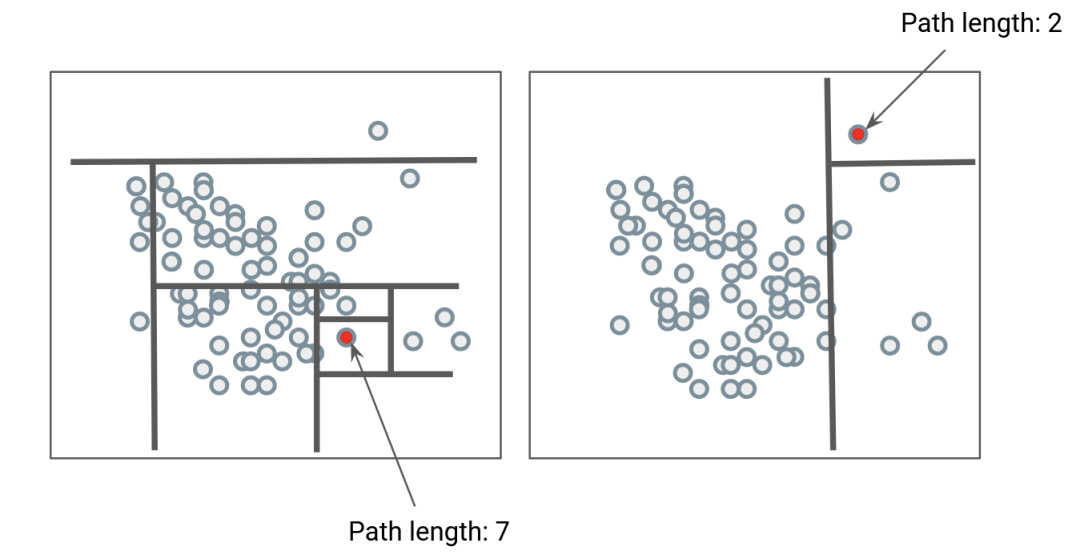
\includegraphics[width=10cm, scale=1]{images/iforest}
	\caption{I-Forest}
	\label{iforest}
\end{figure}
\subsubsection{INNE}
l rilevamento di anomalie basato sull'isolamento utilizzando ensemble di nearest-neighbour (INNE) \cite{bandaragoda2018isolation} è un metodo per rilevare anomalie in cui un ensemble di nearest-neighbor viene addestrato sui dati normali per identificare i punti di dati che sono isolati dal resto dei dati, che vengono considerati anomalie.

Il processo di solito funziona come segue:
\begin{enumerate}
\item Il set di dati viene diviso in un insieme di addestramento e di test.
\item L'ensemble di nearest-neighbor viene addestrato sull'insieme di addestramento utilizzando una tecnica come KNN o LOF.
\item L'ensemble di nearest-neighbor viene quindi utilizzato per identificare i punti di dati isolati nell'insieme di test. Questi punti di dati isolati vengono considerati anomalie.
\item Un punteggio di anomalia viene assegnato a ogni punto di dati, basato su quanto è isolato il punto dal resto dei dati. Più alto è il punteggio di anomalia, maggiore è la probabilità che il punto di dati sia un'anomalia.
\end{enumerate}

\subsubsection{Feature-Bagging}
Feature Bagging \cite{lazarevic2005feature} è un meta-estimator che adatta una serie di predittori di base a vari sotto-insiemi del dataset ed utilizza la media o altri metodi di combinazione per migliorare l'accuratezza predittiva e controllare l'over-fitting.
Le feature sono anch'esse campionate in modo casuale.
Per impostazione predefinita, viene utilizzato LOF come predittore di base. Tuttavia, è possibile utilizzare qualsiasi modello, come KNN e ABOD.
Il Feature Bagging costruisce innanzitutto \textit{n} sottoinsiemi selezionando casualmente un sottoinsieme di feature, il che induce la diversità dei predittori di base.
Infine, il punteggio di predizione viene generato facendo la media o prendendo il massimo.

\section{Modelli a rete neurale}
I metodi basati sulle reti neurali sono una sotto-categoria di metodi di Machine Learning che si basano su reti neurali.
Le reti neurali possono essere considerate come strutture che simulano il comportamento e il meccanismo del cervello umano. Come il cervello umano, l'unità di base della computazione è il neurone e questi sono collegati tra loro attraverso le sinapsi.  Il segnale propagato è proporzionale all'input ricevuto.
In primo luogo, c'è una serie di neuroni che si trovano all'ingresso della rete: questi sono chiamati neuroni di ingresso, che hanno il compito di raccogliere le informazioni da elaborare all'interno della rete.
Poi, c'è un neurone chiamato neurone di uscita, che ha il compito di restituire il risultato della computazione della rete. L'elaborazione avviene, in questo caso attraverso la somma ponderata degli ingressi. 
Ad ogni segnale di ingresso viene associato un peso, che è un punto fondamentale delle reti neurali, in quanto è attraverso questi pesi viene restituito un risultato piuttosto che un altro. Inoltre, al neurone di uscita è associato un ulteriore input chiamato bias: esso rappresenta la tendenza del neurone ad attivarsi o meno. Ovviamente, maggiore è il bias, maggiore è la tendenza del neurone ad attivarsi, poiché aggiunge più informazioni alla somma ponderata. Per semplificare i calcoli, il bias viene trattato come un neurone di ingresso aggiuntivo con segnale di ingresso sempre uguale a 1 e peso associato pari al bias scelto. A questo punto, il risultato della somma ponderata passa attraverso una funzione di attivazione, che restituisce il risultato effettivo.

Ci sono diversi tipi di reti neurali, tra cui:
\begin{itemize}
\item \textit{Reti feed-forward}: una semplice struttura di reti neurali in cui i dati scorrono in una direzione, dall'ingresso all'uscita.
\item \textit{Reti ricorrenti}: una struttura di reti neurali in cui i dati possono fluire in entrambe le direzioni, dall'ingresso all'uscita e viceversa.
\item  \textit{Reti convoluzionali}: una struttura di reti neurali utilizzata per lavorare con immagini e video, in cui vengono utilizzati filtri per estrarre caratteristiche dai dati di ingresso.
\item \textit{Reti autoencoder}: una struttura di reti neurali utilizzata per la riduzione della dimensionalità e l'apprendimento non supervisionato.
\item \textit{Reti generative}: una struttura di reti neurali utilizzata per generare nuovi dati, come ad esempio immagini, testo o suoni.
\end{itemize}


\subsection{Reti neurali profonde}
Le reti neurali vengono definite profonde quando hanno molti strati di neuroni. In generale, si considera una rete neurale profonda quando ha almeno tre strati nascosti, ovvero strati tra l'ingresso e l'uscita della rete. Un numero maggiore di strati consente alla rete di apprendere rappresentazioni più complesse dei dati.
\subsubsection{DeepSVDD}
\begin{figure}[t]
	\centering
	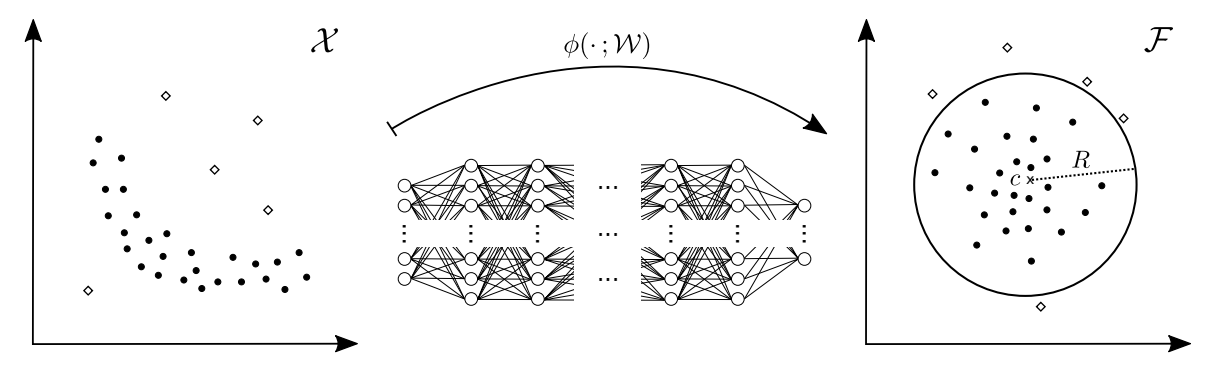
\includegraphics[width=10cm, scale=1]{images/deepsvdd}
	\caption{DeepSVDD}
	\label{deepsvdd}
\end{figure}

Deep Support Vector Data Description (DeepSVDD) \cite{ruff2018deepsvdd} è una rete neurale profonda che durante la fase di training punta a minimizzare il volume della ipersfera che racchiude la rappresentazione sui dati. Minimizzare il volume dell'ipersfera forza la rete neurale ad estrarre i fattori comuni di variazione dato che deve mappare i punti del dataset al centro della sfera.  La Figura \ref{deepsvdd} mostra le trasformazioni di DeepSVDD.

\subsection{Auto-Encoders}
Un Auto-Encoder (AE) \cite{aggarwal2015outlier} è una rete neurale che combina un encoder $E$ e un decoder $D$. L'encoder è un modulo che comprime i dati. Riceve come input il vettore di dati $W$ inerente ad un'osservazione del dataset e li mappa in un insieme di variabili latenti $Z$ che solitamente sono situati in uno spazio dimensionale minore. Il decoder è il secondo modulo il quale si occupa di decodificare le variabili latenti Z, rimappandole nello spazio originario di input come ricostruzione $\widehat{W}$. La differenza tra il vettore di dati $W$ e il vettore ricostruito $\widehat{W}$ è chiamata \textit{errore di ricostruzione}. Pertanto, l'obiettivo dell'addestramento mira a minimizzare questo errore. Nell'ambito dell'Anomaly Detection, viene utilizzato questo errore come score di anomalia: se un auto-encoder riesce a ricostruire senza errori un sample vuol dire che questo esprime caratteristiche normali; un sample anomalo invece porta l'auto-encoder a compiere errori nella fase di ricostruzione. L'architettura di un auto-encoder è presente nella Figura \ref{ae}.
\begin{figure}[t]
	\centering
	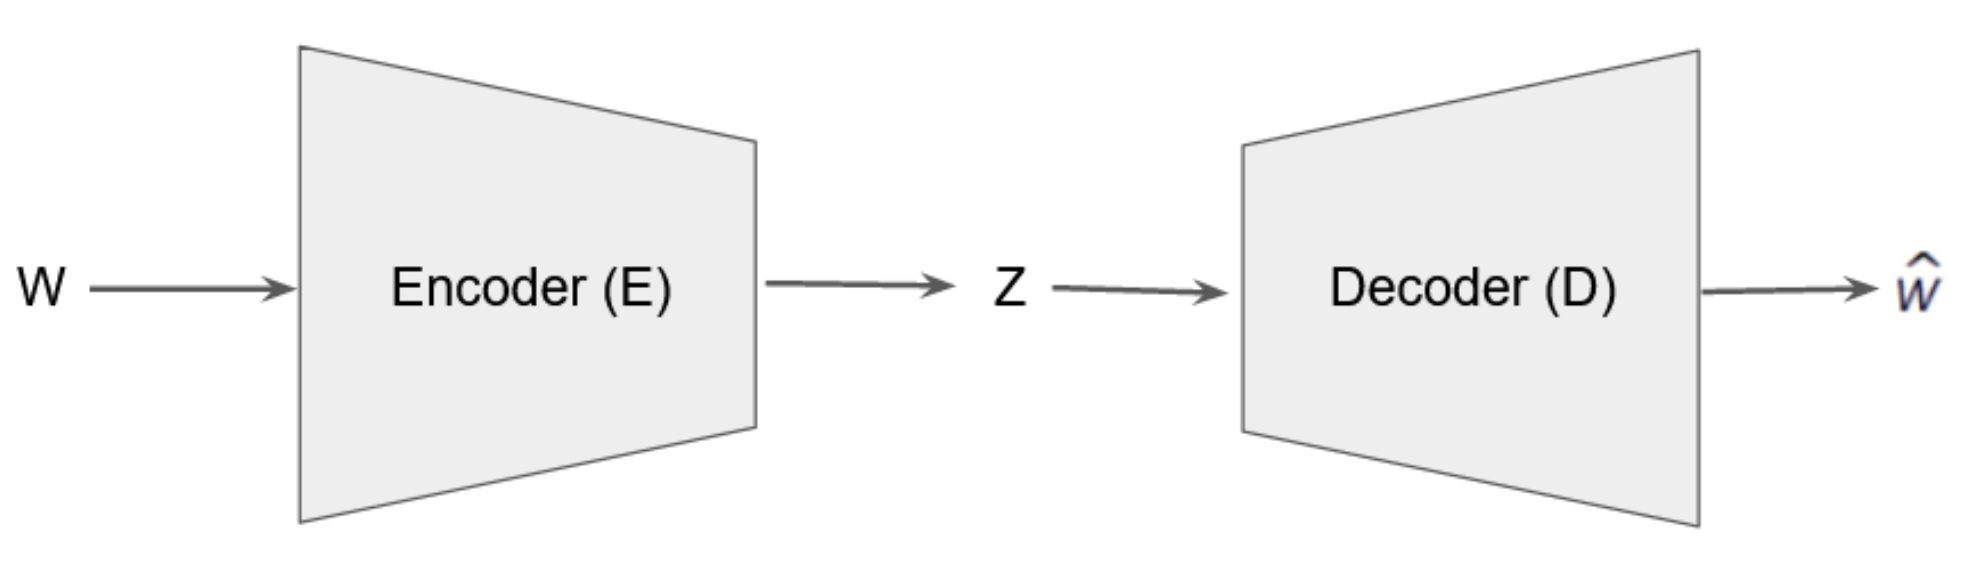
\includegraphics[width=10cm, scale=1]{images/ae}
	\caption{Auto-Encoder}
	\label{ae}
\end{figure}
\subsubsection{Variational-Autoencoders}
I Variational Autoencoders (VAE) \cite{kingma2013auto} ereditano parte dell'architettura dei classici AutoEncoders ma hanno profonde differenze. VAE è considerato un modello generativo e inoltre il suo encoder non solo produce una rappresentazione latente, ma anche una distribuzione di probabilità della rappresentazione latente $\mu$ e $\sigma$. Questo rende possibile generare nuovi sample semplicemente estraendo valori casuali dalla distribuzione di probabilità prodotta dall'encoder.
Il modello viene allenato per minimizzare la divergenza Kullback-Leibler (KL) tra la distribuzione di probabilità prodotta dall'encoder e una distribuzione nota (spesso una distribuzione normale) e allo stesso tempo massimizzare la capacità del decoder di ricostruire l'immagine originale (Figura \ref{vae}).
\begin{figure}[t]
	\centering
	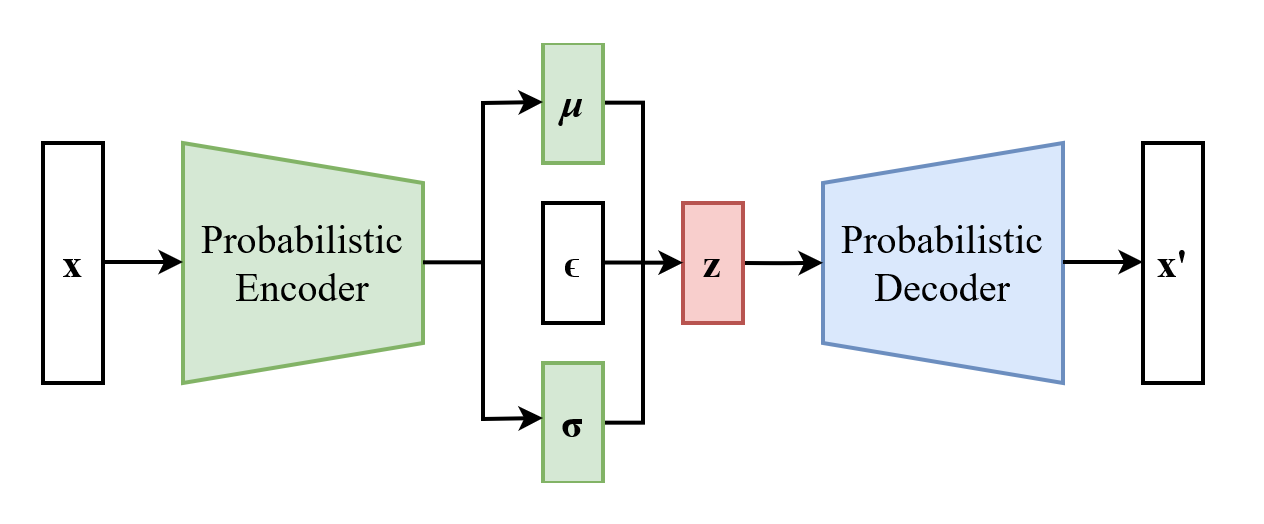
\includegraphics[width=10cm, scale=1]{images/vae}
	\caption{VAE}
	\label{vae}
\end{figure}

\subsection{LSTM}
Le LSTM (Long Short-Term Memory) sono un tipo di rete neurale artificiale utilizzata in problemi di elaborazione del linguaggio e predizione dei dati temporali. Sono state progettate per gestire problemi di "vanishing gradient" presenti in modelli di rete neurale tradizionali, consentendo una memorizzazione a lungo termine dei dati. Ciò significa che le LSTM possono tenere traccia di eventi che accadono molto tempo prima, il che è utile per comprendere il contesto.
Le reti LSTM sono composte da elementi detti \textit{unit} o \textit{celle} che a loro volta sono composte da dei \textit{gates}: uno di ingresso, uno di uscita e uno detto \textit{forget gate}. La cella ricorda i valori su intervalli di tempo arbitrari e i tre gate regolano il flusso di informazioni in entrata e in uscita. Le forget gate decidono quali informazioni scartare da uno stato precedente assegnando a quest'ultimo, rispetto all'ingresso corrente, un valore compreso tra 0 e 1. Un valore vicino a 1 significa mantenere l'informazione, mentre un valore di 0 significa scartarla. Le porte di ingresso decidono quali nuove informazioni memorizzare nello stato corrente, utilizzando lo stesso sistema delle forget gate. Le porte di uscita controllano quali informazioni dello stato corrente devono essere emesse, assegnando un valore da 0 a 1 alle informazioni, tenendo conto degli stati precedenti e di quello attuale. L'emissione selettiva di informazioni rilevanti dallo stato corrente consente alla rete LSTM di mantenere dipendenze utili a lungo termine per fare previsioni, sia nel tempo corrente che in quello futuro.

Le LSTM possono essere utilizzate per rilevare anomalie in dati temporali andando ad addestrare il modello sui dati "normali", per imparare una rappresentazione del comportamento normale dei dati. Quindi, quando nuovi dati vengono presentati al modello, possono essere utilizzati per generare una previsione e confrontare questa previsione con i dati effettivi. Se ci sono differenze significative tra la previsione e i dati effettivi, allora questi dati possono essere considerati anomali.


\subsection{Reti avversarie generative}
Le reti avversarie generative, o in breve GAN, sono un approccio alla modellazione generativa che utilizza metodi di apprendimento come le reti neurali convoluzionali.

La modellazione generativa è un task dell'apprendimento non supervisionato che prevede la scoperta e l'apprendimento automatico delle relazioni o delle variabili latenti all'interno dei dati di input in modo tale che il modello possa essere utilizzato per generare o produrre nuovi esempi che potrebbero essere stati plausibilmente ricavati dal set di dati originale.

Le GAN sono un modo di addestrare un modello generativo strutturando il problema in due parti: il modello generatore, che viene addestrato per generare nuovi esempi, e il modello discriminatore, che cerca di classificare gli esempi come reali (provenienti dal dominio) o falsi (generati). I due modelli vengono addestrati insieme in un gioco a somma zero (da qui adversarial), fino a quando il modello discriminatore viene ingannato circa la metà delle volte, il che significa che il modello generatore sta generando esempi plausibili. Lo schema della rete è presente in Figura \ref{gan}.
\begin{figure}[t]
	\centering
	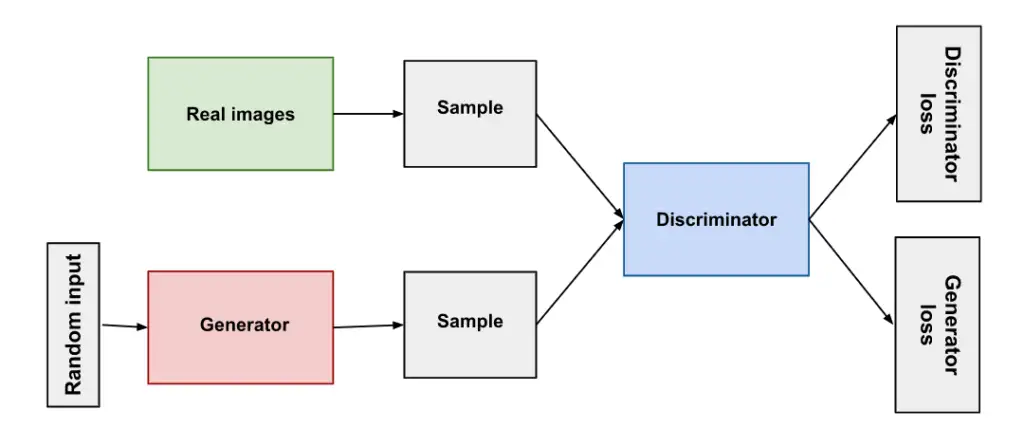
\includegraphics[width=12cm, scale=1]{images/gan}
	\caption{GAN}
	\label{gan}
\end{figure}

\subsubsection{AnoGAN}
AnoGAN (Anomaly GAN) \cite{schlegl2017unsupervised} è una tecnica di rilevamento di anomalie basata su GAN. Il modello AnoGAN utilizza un generatore GAN per generare una rappresentazione dei dati normali e quindi utilizza una rete neurale di rilevamento di anomalie per distinguere i dati normali dalle anomalie.

Il modello AnoGAN è composto da tre componenti principali:

\begin{enumerate}
\item Il generatore GAN che impara a generare dati che seguono la distribuzione dei dati normali.
\item Il discriminatore GAN che impara a distinguere i dati generati dai dati reali.
\item La rete neurale di rilevamento di anomalie che utilizza la rappresentazione generata dal generatore GAN per distinguere i dati normali dalle anomalie.
\end{enumerate}


\subsubsection{ALAD}
Adversarially Learned Anomaly Detection (ALAD) \cite{zenati2018adversarially} è una rete neurale che basa le sue fondamenta su AnoGAN. Ma a differenza di quest'ultima, include una GAN bi-direzionale e di conseguenza è presente un encoder al suo interno che mappa i dati di input in uno spazio latente ed utilizza l'errore di ricostruzione come score di anomalia.

\subsection{Reti neurali a grafo}
Le reti neurali basate su grafi (o GNN, Graph Neural Networks) sono una classe di modelli di apprendimento automatico che utilizzano strutture di dati a forma di grafo per rappresentare i dati. In questi modelli, i nodi del grafo rappresentano i sample e gli archi rappresentano le relazioni tra questi. Le GNN utilizzano un algoritmo di propagazione per aggiornare i valori dei nodi del grafo in base alle informazioni che si trovano sui nodi adiacenti.

\subsubsection{LUNAR}
LUNAR: Unifying Local Outlier Detection Methods via Graph Neural Networks \cite{goodge2022lunar} è un metodo per la rilevazione di anomalie che utilizza le reti neurali su grafi per apprendere la struttura locale dei dati. Il metodo si basa sull'idea che i punti di dati normali saranno simili ai loro punti di dati vicini, mentre i punti di dati anomali saranno dissimili.
Il processo di solito funziona come segue:
\begin{enumerate}
\item Viene costruito un grafo dai dati, dove ogni nodo rappresenta un punto di dati e gli archi vengono tracciati tra i punti di dati che vengono considerati simili.
\item Una rete neurale su grafi viene addestrata sul grafo per apprendere la struttura locale dei dati.
\item Dopo l'addestramento, la rete viene utilizzata per calcolare un punteggio di outlier per ogni punto di dati. Il punteggio di outlier rappresenta quanto dissimile è il punto di dati dai suoi punti di dati vicini.
\item I punti di dati con punteggi di outlier elevati vengono considerati anomalie.

\end{enumerate}

 È particolarmente utile per rilevare anomalie in dati che hanno una struttura complessa. Il metodo è in grado di modellare la struttura locale dei dati, il che lo rende efficace nel rilevare anomalie che potrebbero essere mancate da altri metodi.




\section{Thresholding}
Il problema del thresholding nella rilevazione di anomalie si riferisce alla sfida di determinare il valore di soglia appropriato che separi i punti di dati normali dai punti di dati anomali. Il valore di soglia viene solitamente utilizzato per assegnare un'etichetta di anomalia a ciascun punto di dati: i punti di dati con score di anomalia superiori alla soglia vengono considerati anomalie. Tuttavia, determinare il valore di soglia appropriato può essere difficile, poiché dipende dall'applicazione specifica e dall'insieme di dati.

Una delle principali sfide del thresholding è che solitamente si basa su una conoscenza a priori dei dati, che potrebbe non essere disponibile o potrebbe essere inaccurata. Inoltre, la distribuzione dei punti di dati e il numero di punti di dati anomali possono variare notevolmente tra diversi set di dati, rendendo difficile determinare un valore di soglia appropriato per tutti i set di dati.

Un'altra sfida del thresholding è che può essere difficile bilanciare il compromesso tra il numero di rilevamenti true-positive ed il numero di rilevamenti false-positive. Un valore di soglia troppo alto può causare molti falsi negativi, mentre un valore di soglia troppo basso può causare molti falsi positivi.
Sono proposti ora due metodi classici di thresholding ed un terzo metodo che verrà utilizzato nel Model Selection.

\subsection{IQR}
IQR \cite{https://doi.org/10.48550/arxiv.1509.02473} si basa sull'uso della deviazione interquartile (che è la differenza tra il terzo e il primo quartile) come base per determinare se un punto di dati è anomalo.

Il processo funziona come segue:
\begin{enumerate}
\item Viene calcolato il primo quartile (Q1), il terzo quartile (Q3) dei dati e la deviazione interquartile IQR dove $IQR = Q3-Q1$.
\item Viene definita la soglia inferiore come $Q1 - 1.5 \cdot IQR$ e la soglia superiore come $Q3 + 1.5 \cdot IQR$.
\item I punti di dati che si trovano al di fuori del range tra la soglia inferiore e la soglia superiore vengono considerati anomalie.
\end{enumerate}

Il vantaggio di questo metodo è che si basa solo sui dati e non richiede alcuna conoscenza a priori dei dati, quindi è un metodo semplice ed efficiente per determinare i valori di soglia. Tuttavia, questo metodo è sensibile ai valori estremi, quindi potrebbe non essere adatto per i dati con molti valori estremi.

\subsection{Z-Score}
Z-Score \cite{Bagdonavi_ius_2020} è una misura della distanza di un punto di dati dalla media dei dati in termini di deviazione standard. I punti di dati con Z-Score alti o troppo bassi vengono considerati anomalie.
Il processo funziona come segue:
\begin{enumerate}
\item Viene calcolata la media e la deviazione standard dei dati.
\item Viene calcolato lo Z-Score per ogni punto di dati utilizzando la formula $(x_i - avg) / std$.
\item Viene definita una soglia per i Z-Score, ad esempio 3 o -3 (che rappresentano rispettivamente 3 deviazioni standard sopra o sotto la media).
\item I punti di dati con Z-Score al di fuori della soglia vengono considerati anomalie.
\end{enumerate}
Anche questo metodo si basa solo sui dati e non richiede alcuna conoscenza a priori. Tuttavia, questo metodo presuppone che i dati seguano una distribuzione normale, quindi potrebbe non essere adatto per i dati non normalmente distribuiti. Inoltre, il valore della soglia deve essere scelto con attenzione in quanto può avere un impatto significativo sulle prestazioni del metodo.


\section{\texorpdfstring{$\gamma$}-GMM}
"ESTIMATING THE CONTAMINATION FACTOR’S DISTRIBUTION IN UNSUPERVISED ANOMALY DETECTION" \cite{https://doi.org/10.48550/arxiv.2210.10487} è un paper pubblicato da Lorenzo Perini et al.
Il problema trattato in questo paper consiste nella stima della distribuzione del fattore di contaminazione ($\gamma$) di un dataset non etichettato utilizzando un insieme di M rilevatori di anomalie non supervisionati. 
Per fattore di contaminazione si intende il valore, espresso in percentuale, della quantità di punti anomali in un dataset. 

Per affrontare questo problema, in questo paper viene proposto $\gamma$GMM, un approccio innovativo che utilizza un metodo bayesiano per stimare la distribuzione del fattore di contaminazione.
L'approccio $\gamma$GMM si compone di quattro fasi:
\begin{enumerate}
\item La prima fase consiste nella mappatura dei dati in uno spazio di anomalie a M dimensioni, dove le dimensioni corrispondono ai punteggi di anomalia assegnati dai M rilevatori di anomalie. In questo spazio, il pattern evidente è che "più alto è il punteggio, più anomalo è il dato".
\item La seconda fase consiste nel modellare i dati in questo spazio utilizzando un modello di miscela di Gaussiane con processo di Dirichlet (DPGMM). Si assume che ognuno dei tanti componenti di miscela contenga solo dati normali o solo dati anomali. Se si conoscesse quali componenti contengono anomalie, sarebbe possibile derivare facilmente la distribuzione posteriore di $\gamma$ come somma delle proporzioni di miscela dei componenti anomali. Tuttavia, in questo setting tale informazione non è disponibile.
\item La terza fase consiste nella stima della probabilità che i $k$ componenti più estremi siano anomalie. Ciò presenta tre sfide: (1) rappresentare ogni componente in uno spazio M-dimensionale utilizzando un unico valore per ordinarli dal più anomalo al meno anomalo, (2) calcolare la probabilità che il k-esimo componente sia anomalo dato che il (k-1)-esimo è tale, (3) derivare la probabilità obiettivo che esattamente $k$ componenti siano anomalie congiuntamente.
\item La quarta e ultima fase consiste nella stima della distribuzione posteriore del fattore di contaminazione ($\gamma$) utilizzando la probabilità congiunta e le proporzioni di miscela dei componenti.
Le quattro fasi di lavoro sono mostrate nella Figura \ref{ygmm1}.

\end{enumerate}
\begin{figure}[t]
	\centering
	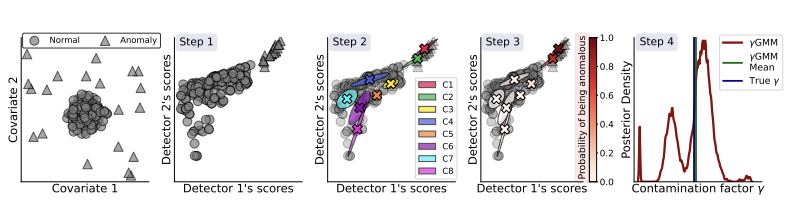
\includegraphics[width=14cm, scale=1]{images/ygmm1}
	\caption{I 4 step di $\gamma$GMM.}
	\label{ygmm1}
\end{figure}

In generale, l'approccio $\gamma$GMM fornisce una stima della distribuzione del fattore di contaminazione ($\gamma$) che può essere utilizzata per quantificare la probabilità che un dato campione sia anomalo rispetto a una distribuzione di dati normali. Inoltre, utilizzando un metodo bayesiano per la stima della distribuzione di $\gamma$, l'approccio $\gamma$GMM tiene conto delle incertezze nei parametri del modello. Ciò consente di ottenere una stima più precisa e robusta del fattore di contaminazione rispetto ai metodi tradizionali.
La formula utilizzata per la stima della distribuzione di $\gamma$ è la seguente:

\[p(\gamma | X) = \sum_{k=1}^{K} p(k | X) \sum_{i_1 < i_2 <...< i_k}^{m} p(\gamma | z_{i_1}, z_{i_2},..., z_{i_k}) p(z_{i_1}, z_{i_2},..., z_{i_k} | X)\]
dove $X$ è l'insieme di dati, $\gamma$ è il fattore di contaminazione, $k$ è il numero di componenti anomali, $z$ è il vettore di appartenenza ai componenti di miscela e $m$ è il numero di componenti di miscela.

All'interno del paper sono presenti anche i risultati degli esperimenti in cui il metodo $\gamma$GMM viene confrontato con numerosi metodi di thresholding tra cui IQR o Z-Score. I risultati sono incoraggianti e non solo ottiene il punteggio di MAE più basso (rispetto al true $\gamma$), ma la degradazione di una metrica supervisionata, come F-Measure, di un rilevatore di anomalie a cui è stato passato come fattore di contaminazione quanto generato dall'algoritmo di $\gamma$GMM, è la più bassa rispetto a tutti gli altri metodi di thresholding (Figura \ref{ygmm2}). 

\begin{figure}[t]
	\centering
	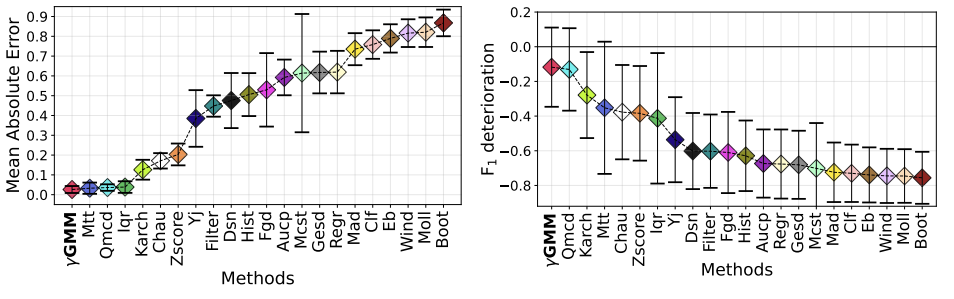
\includegraphics[width=14cm, scale=1]{images/ygmm2}
	\caption{Performance di $\gamma$GMM rispetto ad altre tecniche di thresholding. A sinistra i valori di MAE mentre a destra la F1-Deterioration.}
	\label{ygmm2}
\end{figure}

Per questo motivo, si è deciso di utilizzare questo metodo per la stima di contaminazione dei dati di SKF. Valore che poi è stato utilizzato come parametro ai modelli di Anomaly Detection utilizzato nel Model Selection.

\clearemptydoublepage
\chapter{Model Selection}

\section{Introduzione}
Model Selection è il processo di selezione di un modello finale, che sia di machine learning o deep learning, tra una serie di modelli candidati per uno specifico dataset.

E' un processo che può essere applicato sia a diversi tipi di modelli, ad esempio regressione logistica, SVM, KNN ecc.; sia a modelli dello stesso tipo ma con configurazione di iper-parametri differenti, ad esempio kernel diversi in un SVM.

Model Selection risulta molto utile ed efficace quando si e' interessati nel sviluppare un modello di classificazione o regressione per un dataset, ma non si sa a priori quale modello funzioni meglio. Di conseguenza la soluzione e' quella di fare training e valutazione per ogni modello preso in considerazione.




\section{Supervised Model Selection}
Le metodologie di Model Selection supervisionato sono quelle classiche che di solito vengono applicate durante lo sviluppo di algoritmi di Machine o Deep Learning. Avendo a disposizione le labels, le scelte ricadono dunque su come partizionare il dataset in train/split e validation set, su come pesare la complessita di un modello e su quali metriche di valutazione adottare.

\subsection{Resampling Methods}
I metodi di resampling, come suggerisce il nome, sono semplici tecniche di partizionamento dei dati e servono per valutare se il modello generalizza bene anche sull'insieme di test. Diversi tipi di split possono essere applicati:
\begin{itemize}
	\item \textbf{Random Split}
	\item \textbf{Time Based Split} 
	\item \textbf{K-Fold Cross Validation}
	\item \textbf{Stratified K-Fold}
\end{itemize}
Un approfondimento di queste tecniche e' stato proposto nel capitolo TODO

\subsection{Ottimizzazione degli iper-parametri}
L'ottimizzazione degli iperparametri è il processo di ricerca del miglior insieme di iperparametri per un modello di machine learning. Gli iperparametri sono dei parametri che non vengono appresi dai dati durante l'addestramento, ma vengono impostati prima dell'inizio di questo. Esempi di iperparametri sono il learning rate di una rete neurale, il numero di alberi in una random forest o regularization factor di un modello lineare. Nell'ambito del model selection, l'obiettivo dell'ottimizzazione degli iperparametri è quello di trovare l'insieme di iperparametri che consente di ottenere le migliori prestazioni per il modello in analisi. Ciò può essere fatto utilizzando tecniche come grid search, random search o l'ottimizzazione bayesiana per esplorare lo spazio degli iperparametri e trovare l'insieme ottimale.


\subsection{Probabilistic Methods}
I metodi probabilistici non tengono conto solo delle prestazioni del modello, ma anche della sua complessità. La complessità del modello è misurata dalla capacità di catturare la varianza dei dati. 
Ad esempio, un modello con un bias alto come l'algoritmo di regressione lineare è meno complesso, mentre una rete neurale ha una complessità molto più elevata.
Un altro punto importante da notare è che le prestazioni del modello prese in considerazione nelle misure probabilistiche sono calcolate solo dal set di train. In genere non è necessario un set di test.
Uno svantaggio, invece, risiede tuttavia nel fatto che i metodi probabilistici non considerano l'incertezza dei modelli e hanno la possibilità di selezionare  quelli più semplici rispetto a quelli complessi.
\begin{itemize}
	\item \textbf{Minimum Description Length} o MDL, deriva dalla teoria dell'informazione che si occupa di metriche come l'entropia, che misura il numero medio di bit necessari per rappresentare un evento da una distribuzione di probabilità o da una variabile casuale. 
	      MDL è dunque il numero minimo di bit necessari per rappresentare il modello.
\end{itemize}

\subsection{Metriche di valutazione}
I modelli possono essere valutati utilizzando diverse metriche, tuttavia, la scelta di una metrica di valutazione consona è cruciale e spesso dipende dal problema da risolvere. Una chiara comprensione di un'ampia gamma di metriche può aiutare a trovare una corrispondenza appropriata tra la descrizione del problema ed una metrica.
Per una descrizione delle metriche utilizzabili nel Model Selection, fare riferimento al capitolo TODO

\section{Unsupervised Model Selection}
Tecniche e metriche sopra descritte hanno applicazione solamente quando si ha a disposizione ground truth labels. Spesso pero', e sopratutto nel dominio dell'Anomaly Detection, le labels non sono disponibili e bisogna quindi cambiare completamente approccio. 
Unsupervised Outlier Model Selection, in breve UOMS, ha ricevuto fin'ora poca attenzione da parte dei ricercatori, tant'è' che solamente una manciata di lavori sono stati pubblicati. Queste proposte assumono diversi approcci al problema e possono essere divisi in due categorie: meta learning e metriche surrogate.

\subsubsection{Definizione del problema}
Sia \({x_t,y_t}^T_{t=1}\) un dataset multidimensionale o una serie temporale multivariata con osservazioni (\(x_1,...,x_T\)), \(x_t\in\Re^d\) e label di anomalia (\(y_1,...,y_T\)), \(y_t \in \{0,1\}\), dove \(y_t=1\) indica che l'osservazione \(x_t\) e' anomala. Le labels saranno usate solamente per la fase di valutazione dei metodi proposti e non per la selezione del modello.

Sia \(M=\{A_i\}^N_{i=1}\) un set di N modelli candidati di anomaly detction dove ogni modello \(A_i\) e' una tupla (\(detector, iper-parametri\)) .
I modelli di anomaly detection non necessitano labels per il training e di conseguenza la fase di train/test split puo essere ignorata.  Questi passaggi vengono comunque eseguiti e consideriamo quindi uno split \(\{x_t\}_{t=1}^{t_{test}-1}\),\(\{x_t\}^{T}_{t=t_{test}}\).

Viene assunto che il modello allenato \(A_i\), quando applicato alle osservazioni \(\{x_t\}^{T}_{t=t_{test}}\) , produca degli score di anomalia \(\{s_t^i\}_{t=t_{test}}^T\),\(s^i_t\in\Re_{\geq0}\). Valori piu alti per gli score di anomalia indicano che l'osservazione e' piu probabile essere anomala.
Le performance di un modello possono essere misurate usando una metrica supervisionata \(Q(\{s_t\}^T_{t=1},\{y_t\}^T_{t=1})\) come F1 Score.

Possiamo ora definire il problema come: date le osservazioni \(X_{test}\) ed un set di modelli \(M=\{A_i\}^N_{i=1}\) allenato usando \(X_{train}\), selezionare un modello che massimizzi la misura di qualita' \(Q(A_i(X_{test}),Y_{test})\) senza utilizzo di label per la selezione.

\subsection{Meta Learning}
Questo approccio mira ad identificare il modello migliore per un particolare dataset date le caratteristiche di questo come il numero di classi, attributi, istanze ecc. L'algoritmo si basa su una collezione di dataset storici di outlier detection in cui le labels sono presenti e sulle performance dei modelli su questi per imparare essenzialmente un mapping tra questi due elementi. 
A questo punto l'algoritmo riceve in input il dataset su cui si vuole fare Model Selection (in cui le labels non sono presenti) ed il risultato di output sarà un modello che l'algoritmo ritiene come migliore sulla base di ciò che ha imparato nella fase di analisi sui dataset storici.
Questo metodo pero' richiede quindi la disponibilità di dataset storici con labels e inoltre fallisce se non ne esiste uno che sia sufficientemente rappresentativo del dataset target.
\subsection{Metriche Surrogate}
A differenza del precedente, questo approccio non ha bisogno di dataset storici o di conoscenza pregressa. Ciò su cui si basa e' la definizione di nuove metriche che non hanno bisogno di labels ma che siano correlate con le più classiche metriche supervisionate (Accuracy, Precision, Recall ecc), da qui il termine metriche surrogate.
La definizione di queste metriche non e' triviale, data proprio la loro caratteristica di essere completamente non supervisionate e possono ricadere in categorie completamente differenti tra di loro. Qualche esempio sono: model centrality o performance on injected synthetic anomalies. Un approfondimento su queste metriche e' presente nel capitolo successivo.


\subsection{Rank Aggregation}
Il ranking è alla base di centinaia di algoritmi come Netflix, Amazon e Google. 
Ad esempio, il Search Index di Google, algoritmo per il ranking delle pagine web a seguito di una ricerca da parte di un utente, combina centinaia di misure di ranking e la combinazione di tali misure avviene in genere con un metodo di Rank Aggregation. 
L'obiettivo del Rank Aggregation è riassumere le informazioni dei singoli ranking di input e fornire un'unica classifica finale, che dovrebbe in qualche modo rappresentare un risultato più accurato o veritiero. 

Se si dovesse formulare il task del Rank Aggregation come un problema di ottimizzazione, come prima cosa e' necessario definire una funzione oggetto. In questo costesto, vorremmo trovare una ranking finale che sia piu vicino possibile a tutte i singoli ranking contemporaneamente. In modo formale, si puo definire la funzione come: \[ \Phi(\delta) = \sum_{i=1}^{m} w_id(\delta,L_i), \]	
dove $\delta$ e' un ranking di lunghezza $k=|L_i|$, $w_i$ e' il peso associato alla lista $L_i$, $d$ e' una funzione di distanza e $L_i$ e' la $i^{ma}$ lista ordinata.
L'obiettivo e' di trovare $\delta^*$ che minimizzi la distanza totale tra $\delta^*$ e gli $L_i$
\[ \delta^* = arg min \sum_{i=1}^{m} w_id(\delta,L_i). \]

Selezionare la funzione di distanza piu appropriata e' molto importante e la scelta di solito ricade alla distanza di Kendall.
Intuivamente, la distanza di Kendall viene definita come la sommatoria, per ogni possibile coppia di elementi date due liste in input, della seguente penalita:
se due elementi $t$ e $u$ hanno lo stesso ordinamento in entrambe le liste, allora nessuna penalita viene data. Altrimenti se $t$ precede $u$ in una lista e $u$ precede $t$ nell'altra, allora viene imposta una penalita di 1.
Questa distanza puo assumere valori compresi nell'intervallo $[0,n(n-1)/2]$ e non e' da confodnere con il coefficiente di Kendall. Quest'ultimo, essendo un coefficiente, assume valori nell'intervallo $[-1,1]$ ed e' prevalentemente usato in statistica. Sono due concetti differenti ma correlati da:
\[K_c=1-4K_d/(n(n-1)), K_d = (1-K_c)(n(n-1))/4\]
Quindi quando $K_c=1$ il valore di $K_d$ e' 0, al contrario quando $K_c=-1$ il valore di $K_d$ e' massimo.

Il problema di Rank Aggregation come sopra definito viene anche chiamato "Kemeny-Young problem". Purtroppo e' un problema NP-Hard anche con un numero di ranking basso come 4. Per questo motivo, in questa tesi verranno presentati e usati anche metodi alternativi che approssimino la soluzione in modo più efficiente, come ad esempio Borda. Dettagli su questi metodi saranno esposti nei capitoli successivi.

\subsubsection{Rank Comparison}
Ottenuti i ranking di ogni metrica surrogata e generato il rank finale dopo l'aggregazione, per valutare le performance dell'algoritmo di Model Selection e' necessario comparare i risultati prodotti rispetto ad un rank di riferimento.
In questa tesi saranno usati tre indici differenti applicati o sui ranking di posizione oppure sui ranking contenti gli score prodotti dal Model Selection e saranno:

\begin{itemize}
	\item \textbf{Kendall}: coefficente che usa la distanza di Kendall sopra descritta. Usato sui ranking di posizione
	\item \textbf{Spearman}: usato anche sui ranking di posizione, questo metodo statistico quantifica il grado in cui le variabili sono associate da una funzione monotona, indicando quindi una relazione crescente o decrescete. Viene usato su variabili cardinali e tiene conto dei rank piuttosto che dei dati grezzi.
	\item \textbf{Pearson}: usato sui ranking di score, a differenza di Spearman viene usato solamente su variabili continue e misura una correlazione lineare tra le due variabili.
\end{itemize}

\clearemptydoublepage
\chapter{SKF}
\label{chap:skf}

\section{Introduzione}
SKF è un'azienda multinazionale specializzata nella produzione di cuscinetti a sfera. A seguito della formalizzazione del progetto Beat 4.0 portato avanti da SKF e ALTEN è iniziato un progetto di digitalizzazione degli impianti di produzione attraverso l'installazione di sensori all'interno dei macchinari lungo la catena di montaggio.
Il processo di produzione è composto da varie fasi e parte da due anelli grezzi che costituiranno le parti interne ed esterne del prodotto finale. Entrambi gli anelli vengono raffinati in parallelo attraverso due operazioni sequenziali: la rettifica e la levigatura. 
I due anelli vengono poi assemblati insieme ad altri componenti come la gabbia e gli elementi di rotolamento. Il prodotto finito passa infine attraverso un macchinario il quale esegue misure per valutarne la qualità. 

I dati prodotti dai macchinari sono quindi divisi in due categorie: 
\begin{itemize}
	\item \textbf{CoMo}: dati relativi ai sensori installati sui macchinari di rettifica e levigatura cui fanno riferimento a vibrazione, temperatura, velocità, pressione e scorrimento.
	\item \textbf{MVM}: sono i dati prodotti dai macchinari di controllo qualità sul prodotto finito.
\end{itemize}

Lo scopo di questo progetto e di questa tesi è quello di applicare tecniche non supervisionate di rilevamento anomalie utilizzando i dati a disposizione prodotti dai sensori installati sui macchinari.

\section{Descrizione del dataset}
Poiché i dati sono di proprietà della SKF, la descrizione è ridotta e i nomi delle misure e delle macchine sono fittizi.


\subsection{CoMo}
I dati includono le misurazioni di differenti caratteristiche di alcune delle macchine della catena di produzione. Per ogni macchina monitorata, sono incluse le velocità radiali e assiali, gli inviluppi radiali e assiali, la temperatura, pressione e vibrazione.
Poiché non tutte le macchine dell'impianto sono monitorate vengono persi dettagli e completezza nei dati, ma nonostante questo il dataset a disposizione contiene una grande quantità di dati.
La frequenza di registrazione dei dati CoMo è di 10 minuti. Questo valore così basso porta con se delle problematiche che verranno discusse più avanti, per questo motivo si sta cercando per richiedere di alzare la frequenza.

\subsection{MVM}
I dati di qualità vengono registrati per ogni prodotto che esce dalla catena di produzione.
Le misure di qualità fornite sono quattro bande, indicate con A, B, C e D.
Tutte le bande sono positive per definizione ed ognuna di esse tratta uno specifico tipo di difetto in ogni cuscinetto attraverso l'analisi dello spettro. In particolare:
\begin{itemize}
	\item Banda A riguarda i cosiddetti errori geometrici risultanti dalla fase di rettifica.
	\item Banda B e C riguardano errori nella fase di levigatura.
	\item Banda D trova errori causati dalla presenza di impurità negli oli o liquidi di pulizia usati sui cuscinetti.
\end{itemize}

Considerato la frequenza di uscita di prodotti finiti dalla linea di produzione, i dati MVM sono prodotti ogni due secondi. Questi verranno poi aggregati in intervalli di 10 minuti. La scelta di dieci minuti per la lunghezza del gap temporale non è casuale, infatti è stata fatta per adattarsi alla granularità dei dati CoMo.

\subsubsection{Qualità}
I dati di qualità MVM vengono usati per definire la classe di qualità di appartenenza dei cuscinetti a sfera. Per fare ciò, sono state definite per ogni banda delle soglie alla quale il superamento di una porta il prodotto a ricevere una classificazione di qualità più bassa.
La Tabella \ref{mvm-soglie} mostra come le classi di qualità vengano definite. Per questioni di riservatezza vengono mostrati dei valori di soglia modificati, andando a moltiplicare i valori reali per uno scalare.

\begin{table}
	\caption{\label{mvm-soglie}Soglie bande MVM.}
	\centering
	\begin{tabular}{|l|l|l|l|l|}
		\hline
		Classe & \multicolumn{1}{c|}{Banda A} & \multicolumn{1}{c|}{Banda B} & \multicolumn{1}{c|}{Banda C} & \multicolumn{1}{c|}{Banda D} \\ \hline
		Q1     & 25                           & 7.2                          & 7.2                          & 3.6                          \\ \hline
		Q2     & 36                           & 18.2                         & 18.2                         & 5.2                          \\ \hline
		Q3     & 48                           & 25.6                         & 25.6                         & 12                           \\ \hline
		Q4     & 72                           & 36                           & 36                           & 20                           \\ \hline
	\end{tabular}
\end{table}

Valori di banda più bassi indicano una qualità maggiore, di conseguenza la classe Q1 rappresenta i prodotti migliori mentre la classe Q4 rappresenta gli scarti. 
Per passare da una classe alla successiva è necessario che solamente una delle 4 bande superi il valore di soglia. 
La Tabella \ref{mvm-esempio} mostra un esempio di come le classi vengano computate.

\begin{table}
	\caption{\label{mvm-esempio}Esempio di associazione di Classe qualità.}
	\centering
	\begin{tabular}{|l|l|l|l|l|l|}
		\hline
		Bearing & \multicolumn{1}{c|}{Banda A} & \multicolumn{1}{c|}{Banda B} & \multicolumn{1}{c|}{Banda C} & \multicolumn{1}{c|}{Banda D} & Qualità \\ \hline
		B1      & 20                           & 7                            & 4                            & 2                            & Q1      \\ \hline
		B2      & 19                           & 18                           & 2                            & 5.8                          & Q3      \\ \hline
		B3      & 70                           & 20                           & 20                           & 22                           & Q4      \\ \hline
	\end{tabular}
\end{table}

\section{Processamento dei dati}
I dati sono ricevuti da SKF in formato tabellare e sono suddivisi in dati CoMo e dati MVM. Ogni riga della tabella della qualità corrisponde a un cuscinetto analizzato dalla macchina di qualità, invece le colonne sono costituite dalla data e ora di registrazione dei valori e dalle quattro bande.
La tabella CoMo invece contiene le misure del Condition Monitoring in formato non pivotante: ogni riga corrisponde a un singolo record contenente l'ora del record, il nome della macchina a cui il record si riferisce, il nome della feature misurata e il valore registrato.

Considerando il formato grezzo dei dati, è necessario eseguire diverse trasformazioni per produrre dati pronti al processamento da parte di algoritmi di Machine Learning. 

Prima di entrare nel dettaglio è però necessario condividere alcune osservazioni sulle proprietà dei dati.

\subsection{Proprietà}

\subsubsection{Parzialità dei dati}
Solamente una parte delle macchine del canale di produzione viene monitorata, di conseguenza i dati CoMo a disposizione non sono esaustivi di tutti macchinari che effettuato la levigatura o la rettifica. Al contrario, tutte le registrazioni di qualità MVM sono invece disponibili.

\subsubsection{Frequenza di registrazione}
I vari tipi di sensori non registrano con la stessa frequenza di registrazione e allo stesso momento.
È quindi necessario appiattire i timestamp e aggregare alcuni dati per fare in modo che ogni riga corrisponda alle misure di tutti i sensori monitorati nel periodo di riferimento.


\subsubsection{Frequenza di produzione}
La frequenza di produzione cambia nel tempo. Se vengono aggregati i dati di qualità con intervalli di tempo di 10 minuti, il numero di registrazioni in ogni intervallo è la quantità di cuscinetti analizzati dal monitoraggio.
Poiché ogni cuscinetto prodotto passa attraverso le macchine di qualità, questa quantità è ovviamente correlata alla velocità media di produzione
lungo l'intervallo di tempo considerato. 

Il motivo principale per cui la velocità media di produzione è interessante è che può essere utilizzata come indicatore del fatto che il canale è stato inattivo lungo nell'intervallo di dieci minuti considerato. In particolare, se la velocità media di produzione di un intervallo è significativamente più piccola del solito, indicherà che la produzione è stata interrotta nel periodo considerato. Le possibili cause di tale sospensione possono essere un malfunzionamento, la manutenzione o anche la chiusura programmata del canale.
Per quanto riguarda la quantità di cuscinetti analizzati dalla macchina di qualità monitorata, è vero che, se il processo di produzione è stato sospeso, questa quantità sarà bassa, ma non si può dire con certezza l'opposto.
Questa misura fornisce comunque alcuni indizi sull'attività del canale. Per esempio, esplorando il set di dati, si può notare che la quantità menzionata vada a zero ogni domenica dalle 12:00 alle 22:00 circa, conseguenza del fatto che in quel periodo di tempo c'è stato un turno di riposo. Questo viene confermato anche analizzando i dati CoMo nello stesso periodo temporale: numerosi sensori che producono valori a 0 oppure non li producono affatto, mentre quelli della temperatura iniziano a declinare. 

Queste osservazioni possono essere utilizzate per rilevare i turni di riposo e potenzialmente anche per le fasi di manutenzione, anche se per questi ultimi la rilevazione è di fatto impossibile. In particolare, le manutenzioni sono state registrate su carta, per cui non è possibile sfruttare questi dati come risposta e di conseguenza non è possibile convalidare statisticamente alcuna ipotesi.
Inoltre, la maggior parte delle manutenzioni dura meno di 10 minuti e
non disponendo di dati ad alta frequenza, è quasi sempre impossibile
osservare qualsiasi cambiamento nel comportamento delle serie temporali CoMo. 

\subsubsection{Dati Mancanti}
Per alcuni sensori sono disponibili solo poche settimane di dati e di conseguenza devono essere scartati. Per la parte restante dei dati, escludendo i tempi di inattività, in media il 15\% dei sensori è mancante in un dato momento e ogni misura è mancante in media il 17\% delle volte. Considerato anche quanto detto nel paragrafo precedente, esistono diverse cause possibili per cui un sensore non registra alcun valore in un dato momento. Per esempio, un errore nella configurazione dei sensori, è in corso il turno di riposo ed è possibile che lo stesso accada anche durante le manutenzioni o i crash della macchina.
In generale, non è chiaro come questi eventi possano influenzare l'attività dei sensori. D'altra parte, i sensori potrebbero essere semplicemente mal funzionanti o instabili, così come ci potrebbero essere problematiche nella memorizzazione dei dati all'interno del server locale. 
In conclusione, riuscire a decodificare le reali motivazioni per cui si ha una mancata registrazione potrebbe migliorare in maniera significativa le performance di algoritmi di Machine Learning. Purtroppo a causa della bassa frequenza di registrazione e data la non possibilità di interagire con i tecnici dell'impianto di produzione per queste questioni, sono state messe in atto solamente delle semplici operazioni di processamento.

\subsubsection{Andamento Serie Temporali}
Le serie temporali di SKF presentano un comportamento stabile nel tempo. Come mostrato in Figura \ref{sensors_plot}, elementi di stagionalità non sono presenti e non vi è presenza di trend e quindi le serie possono riferirsi stazionarie. Ipotesi confermata anche dall'esecuzione del test Augmented Dickey-Fuller nel quale veniva rifiutata la Null Hypothesis (la Null Hypothesis affermava la NON stazionarietà dei dati).
Per questo motivo, nelle fasi di processamento, operazioni di decomposizione delle serie temporali non sono state fatte.
È possibile comunque notare un'alta variabilità dei dati all'interno della singola serie temporale, con fluttuazioni più o meno visibili.
\begin{figure}[t]
	\centering
	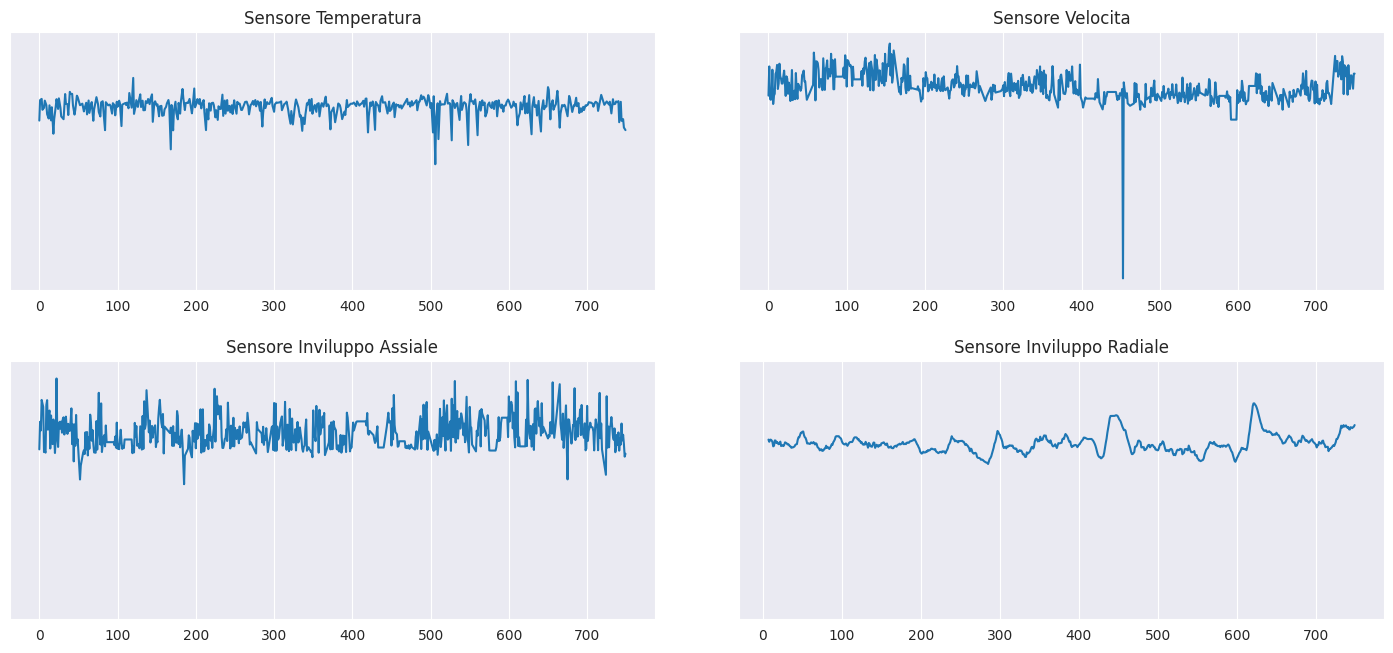
\includegraphics[width=14cm, scale=1]{images/sensors_plot}
	\caption{Andamento Serie Temporali}
	\label{sensors_plot}
		
\end{figure}

\subsection{Processamento}
Evitando i dettagli per questione di riservatezza, in questa sezione vengono presentati i passaggi principali eseguiti per produrre i set di serie temporali dai dati grezzi ricevuti da SKF. 
Per creare una tabella contente una colonna per ogni sensore e con un indice temporale è necessario appiattire i timestamp fino a raggiungere una granularità di 10 minuti, in modo che il tempo possa essere utilizzato come chiave per l'unione. A questo punto ogni riga del dataset corrisponde a un'istantanea di un particolare sensore anche se questa è chiaramente un'approssimazione: in pratica, le registrazioni di misure CoMo diverse non avvengono nello stesso istante, ma la maggior parte di esse si concentra in un intervallo di un minuto circa. 
D'altra parte, i dati sulla qualità sono raccolti in tempo reale quando viene analizzato ogni cuscinetto. In questo caso è quindi necessario aggregare questi dati secondo una qualche misura ed è stata scelta l'operazione di media.
Chiaramente, i dati MVM forniscono informazioni sull'intero intervallo di tempo mentre dati CoMo forniscono invece un'istantanea all'interno dell'intervallo di tempo.
Nell'unire queste misure si è ipotizzato che l'istantanea sia rappresentativa dell'intervallo di tempo ma a causa dell'alta variabilità della maggior parte delle serie temporali, questa ipotesi è lontana dalla realtà.
Questa condizione è molto distante da una situazione ottimale, per questo motivo si sta cercando per spingere a portare la frequenza di registrazione ad uno al minuto. Frequenze più alte consentiranno all'ipotesi sopra descritta di essere valida.

Allo stesso modo in cui sono stati aggregati i dati MVM, può capitare anche all'interno dei dati CoMo che più record dello stesso sensore possano ricadere nello stesso intervallo di tempo. In questo, per ogni tipologia di sensore è stata scelta una funzione di aggregazione tra massimo, minimo e media. La scelta è stata fatta pensando a quali potessero essere i valori più informativi per la caratteristica. Ad esempio, le pressioni sono state sono state aggregate con la funzione di massimo, poiché è probabile che le anomalie siano dei valori elevati; mentre per i flussi è stata scelta la funzione di minimo. Nei casi dubbi l'aggregazione è stata effettuata attraverso la funzione di media.

Dopo i passaggi precedenti, è possibile fare il pivoting della tabella CoMo  prendendo il timestamp come indice di riga. Il risultato è una tabella in cui ogni colonna corrisponde a una serie temporale. 
Come passo finale è necessario trattare i valori mancanti:
\begin{itemize}
	\item Nel caso di intervalli più lunghi di 8 ore con almeno il 50\% di valori mancanti, questi vengono eliminati dal dataset. L'obiettivo è quello di pulire il dataset dai dati registrati durante i turni di riposo in quanto non è di nostro interesse rilevare anomalie in quei intervalli di tempo.
	\item Tutti gli altri valori nulli vengono interpolati linearmente.
\end{itemize}
A questo punto i sensori vengono raggruppati per macchinario, andando quindi a produrre una tabella per ogni macchina.
Come ultimo passaggio si è deciso di andare a normalizzare i valori utilizzando un MinMax Scaler. Questa tecnica permette di normalizzare i valori passando il range del codominio della funzione come parametro di input, in questo caso [0,1]. La formula è definita come:
\[X_{scaled} = (X - X.min(axis=0)) / (X.max(axis=0) - X.min(axis=0))\]

Il valore originario massimo assumerà valore 1, quello minimo 0 e tutti gli altri un valore compreso.
Questo passaggio è necessario in quanto i sensori producono range di valori molto diversi tra di loro e range molto grandi rischiano di andare a pesare di più rispetto a sensori con range bassi. Stringendo il range tra 0 e 1 per tutti i sensori viene risolto questo problema.
\clearemptydoublepage
\chapter{Sperimentazione}
\label{chap:impl}

In questo capitolo viene discussa l'implementazione e l'applicazione delle metriche di Model Selection e delle tecniche di Rank Aggregation. Infine viene proposta una valutazione su dataset di benchmark e quello di SKF.

Riassumendo, questo capitolo si dividerà in:
\begin{enumerate}
	\item Definizione e implementazione delle metriche surrogate per il Model Selection e delle tecniche di Rank Aggregation.
	\item Valutazione su dataset benchmark.
	\item Valutazione su SKF.
\end{enumerate}


\section{Implementazione}
Come introdotto nel Capitolo \ref{chap:modelselection}, il task da risolvere è l'implementazione di un metodo di Model Selection non supervisionato che scelga il modello dato un dataset. L'approccio scelto è stato quello di definire delle metriche "surrogate" che siano correlate con metriche supervisionate e che non richiedano etichette. Le metriche proposte sono indipendenti tra di loro ed è necessario usarne una come candidata oppure aggregarle secondo qualche criterio. Vengono quindi proposti diversi metodologie di Rank Aggregation. Uno schema rappresentante il flusso operazionale è rappresentato in Figura \ref{flow-scheme}.
\begin{figure}[t]
	\centering
	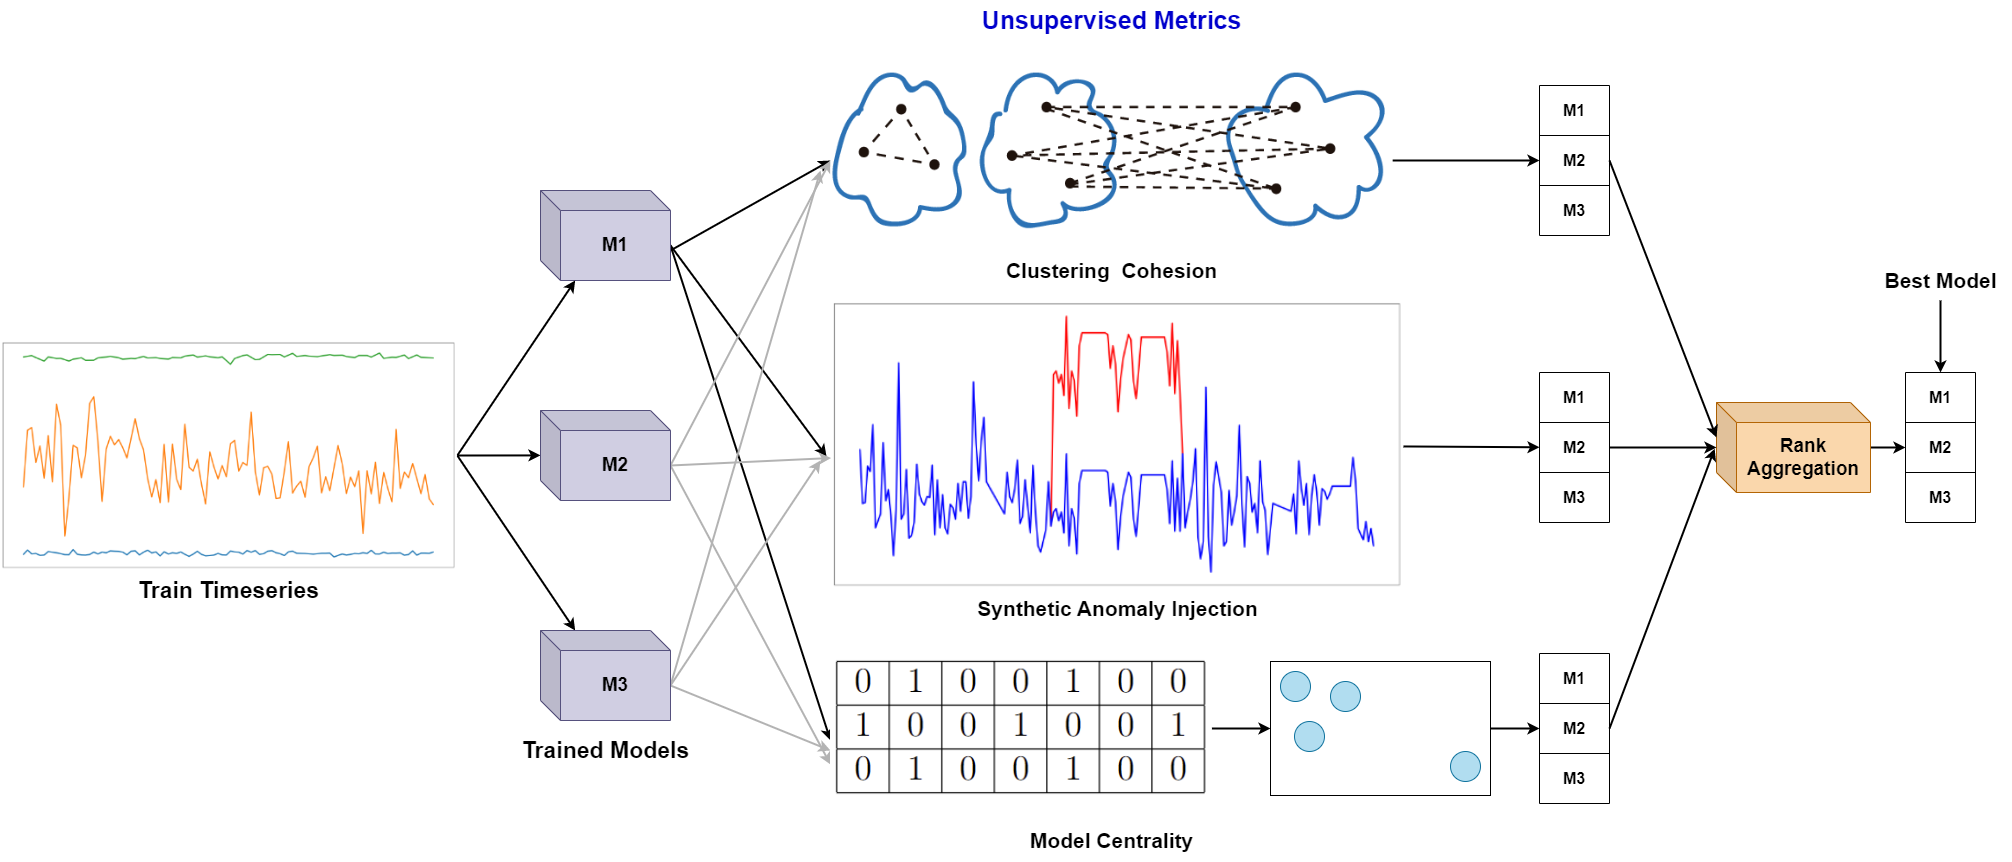
\includegraphics[width=14cm, scale=1]{images/model-selection-scheme}
	\caption{Flusso operazionale}
	\label{flow-scheme}
		
\end{figure}

\subsection{Metriche surrogate}
Ogni metrica non supervisionata serve come misura della bontà di un modello e riduce il problema del Model Selection ad una selezione di quello con lo score più alto. 
Sono state identificate tre classi di metriche e vengono definite non supervisionate in quanto non richiedono etichette. Tuttavia, due di queste utilizzano internamente lo F1 Score, tipicamente utilizzato per la valutazione supervisionata; per evitare confusione viene quindi utilizzato il termine "surrogato".
Di seguito viene analizzata ogni classe di metriche surrogate. 


\subsubsection{Model centrality}
\textit{Esiste una sola ground truth, quindi i modelli vicini a questa sono anch'essi vicini tra loro ed il modello più "centrale" è il migliore.}
Metodi basati sulla centralità hanno ottenuto successi recenti nel Model Selection e nell'Anomaly Detection \cite{DBLP:journals/corr/abs-2104-01422}. 
Per adottare quest'idea si è fatto uso di diverse tecniche che andassero a produrre delle classifiche nella quale i modelli con score più alto erano indicati come quelli più "centrali".
Sono state proposti 4 metodi per computare lo score di Model Centrality. Ognuna di queste riceve come input un set di $K$ modelli a cui è stato fatto training non supervisionato su un dataset di riferimento. 
\begin{itemize}
	\item \textbf{Round Robin}: dati i $K$ modelli, ognuno di questi viene selezionato a turno e le sue etichette prodotte vengono usate come ground truth per valutare le performance degli altri $K-1$ modelli. Infine viene prodotto un'unica classifica finale andando a calcolare la media delle performance di ogni modello rispetto alle $K-1$ iterazioni. 
	\item \textbf{Majority Vote} è il metodo più semplice per generare consenso: dati $K$ modelli e le loro etichette, viene generato un nuovo set di labels finale andando a prendere, per ogni sample, l'etichetta che riceve più voti. Questo nuovo set viene usato come ground truth per valutare i $K$ modelli.
	\item \textbf{Sampling}: per ogni sample all'interno del dataset viene scelto in maniera casuale un modello da usare per estrarne l'etichetta. Viene quindi prodotto un nuovo set di labels da usare come ground truth per valutare i $K$ modelli. Questo metodo si può vedere come: per un dato punto, l'etichetta che appare più volte (nei modelli) viene scelta con più probabilità.
	\item \textbf{Score Correlation}: questo metodo utilizza gli score prodotti da ogni modello, dove lo score, al contrario delle etichette, rappresenta un valore direttamente proporzionale alla probabilità che quel sample sia anomalo. Inizialmente vengono calcolati i ranking di posizione per ognuno di questi set di score: sia $\sigma_{k(i)}$ il rank del sample $i$ secondo gli score prodotti dal modello $K$. Viene poi definita la distanza dal modello $A_k$ al modello $A_l$ come la distanza di Kendall, ovvero il numero di disaccordi per ogni possibile coppia tra i rank di posizione dei due modelli. Infine viene misurata la centralità di un modello come la distanza media rispetto a tutti gli altri modelli.
\end{itemize}

Ognuno di questi metodi produce un ranking finale per cui i modelli con lo score più alto sono quelli più centrali. In particolare i metodi Round Robin, Majority Vote e Sampling, che generano un set di etichette pseudo reali, utilizzano lo F1 Score per valutare ogni modello rispetto a questo set.

Questa metrica surrogata non è perfetta, mentre funziona bene quando i modelli candidati sono tutti sufficientemente buoni da un punto di vista delle performance; nel caso siano presenti un numero relativamente alto di modelli "non buoni", questi potrebbero produrre risultati simili e formare un cluster che va di fatto a condizionare la centralità.
Nella parte della valutazione su dataset di benchmark verranno analizzate le performance di ognuna di queste quattro metodologie.


\subsubsection{Performance on injected synthetic anomalies}
\textit{Un buon modello di Anomaly Detection si comporterà bene anche su dataset con anomalie iniettate sinteticamente}. Alcuni paper hanno precedentemente esplorato l'uso dell' iniezione di anomalie sintetiche per addestrare modelli di rilevamento delle anomalie \cite{DBLP:journals/corr/abs-2107-07702}. Attraverso questa metrica surrogata, viene estesa questa linea di ricerca valutando sistematicamente la capacità dell'algoritmo di Model Selection dopo aver iniettato diversi tipi di anomalie. Dato un dataset di input senza etichette, vengono iniettate casualmente anomalie. La posizione dell'anomalia iniettata viene trattata come un'etichetta pseudo-positiva, mentre il resto dei punti sono trattati come punti pseudo-negativi. 
Infine ogni modello viene valutato attraverso lo F1 Score rispetto alle pseudo-etichette.

Invece di affidarsi a modelli generativi complessi \cite{DBLP:journals/corr/abs-2002-12478}, è stato sviluppato un semplice algoritmo che inietta anomalie di diverso tipo andando prima ad analizzare il dataset ricevuto in input. I tipi di anomalie iniettate prese in considerazione sono 3 e sono visibili in Figura \ref{tipi-anomalie}: 
\begin{figure}[t]
	\centering
	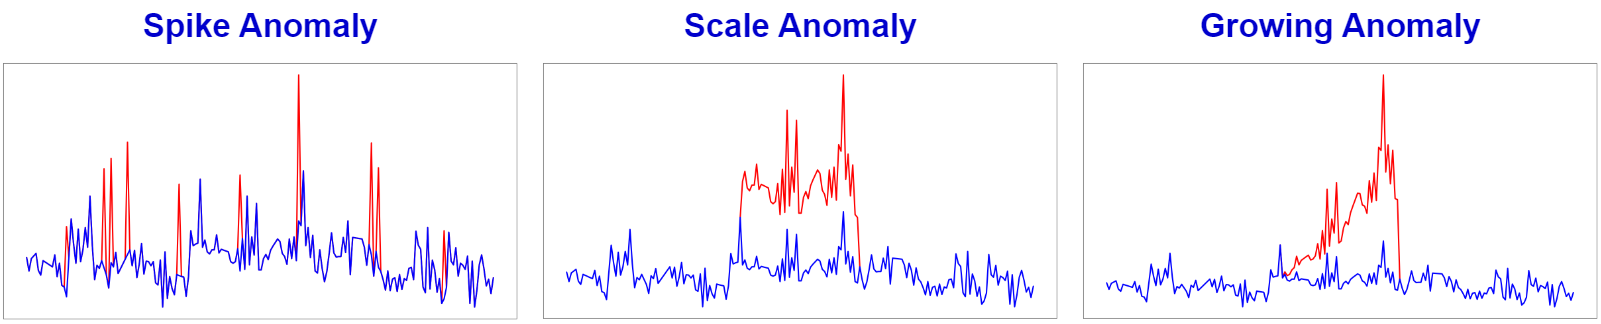
\includegraphics[width=14cm, scale=1]{images/anomalies}
	\caption{Tipologie di anomalie}
	\label{tipi-anomalie}
		
\end{figure}


\begin{enumerate}
	\item \textbf{Spike Anomaly} sono delle anomalie a punto in cui il valore nel punto si discosta in maniera significativa rispetto all'intorno. Lo spike viene generato nel seguente modo: \[ts_a[i] = ts[i] * rnd(1.5, 3) \]
 dove $i$ è un punto nella serie temporale. Nel caso in cui lo spike venga generato verso il basso, il valore casuale rientra nell'intervallo $[0.3,0.5]$.
	\item \textbf{Scale Anomalies} è un intervallo di punti anomali in cui il  valore medio dei punti al suo interno è significativamente più grande o più piccolo rispetto all'intorno. I dati vengono scalati \[ ts_a[start:end] = ts[start:end] * factor \] dove \textit{factor} è sempre un valore casuale nell'intervallo $[1.5,3]$ nel caso di anomalie verso l'alto e $[0.3,0.5]$ nel verso opposto. 
	\item \textbf{Growing Anomalies} è un intervallo di punti anomali in cui il valore di essi cresce o decresce linearmente nel tempo. I dati vengono modificati secondo \[ ts_a[start:end] =  ts[start:end] + linear\_vector \] 
 Dove $linear\_vector$ è un vettore della stessa lunghezza dell'intervallo che si va a modificare in cui i valori crescono linearmente da un valore di base $0$ fino ad un valore di massimo di $0.5$. Nel caso in cui i valori della serie temporale debbano essere portati verso il basso si utilizza l'intervallo $[-0.5,0]$.
\end{enumerate}

I valori scelti a mano per alterare le serie temporali sono frutto di considerazioni svolte sui dati di SKF e poi mantenuti anche su tutti i dataset di benchmark. Chiaramente metodi e valori differenti per l'iniezione di anomalie genereranno risultati che possono essere di molto differenti.
Uno sviluppo futuro potrebbe concentrarsi a sviluppare tecniche più raffinate per l'iniezione di anomalie, in questa tesi si è cercato di mantenere il processo di iniezione il più semplice possibile.

Altro aspetto da tenere in considerazione è il fatto che le anomalie vengono iniettate sui dati scalati nell'intervallo $[0,1]$, generando quindi valori che potrebbero uscire da questo intervallo. Per risolvere a questo problema si è deciso di applicare prima una funzione di \textit{clip}, ovvero i dati modificati vengono limitati ad un range di $[-0.1,1.1]$, e dopo viene ri-eseguita la funziona di normalizzazione nell'intervallo $[0,1]$. Il primo passaggio consente che i nuovi spike o valori estremi vengano effettivamente mantenuti, il secondo passaggio invece riporta all'intervallo desiderato i nuovi valori.

Il numero di anomalie da iniettare viene calcolato sulla base del fattore di contaminazione associato ad un determinato dataset. Ad esempio, su un dataset con 1000 sample ed un fattore di contaminazione di 0.05(5\%), 50 anomalie saranno iniettate.
La posizione nella quale vengono iniettate le anomalie a Spike viene scelta casualmente; invece per quanto riguarda le anomalie a Scale e Growing, vengono generati casualmente dei punti di inizio intervallo mentre la lunghezza di questi è predisposta a mano in base alla frequenza dei sample o alla dimensione del dataset.

Attraverso uno studio di correlazione fra le feature del dataset si è andati a scoprire se due o più feature dovessero essere considerate insieme quando si aggiunge un'anomalia in un determinato punto. In un esempio pratico, se la feature della Pressione e quella del Flusso hanno una correlazione vicina a -1, quindi negativa, l'iniezione dell'anomalia prevede che una delle due feature vede il suo valore modificato verso l'alto mentre l'altro verso il basso. La Figura \ref{feature-correlazioni} mostra un esempio di correlazioni positiva e negativa.
\begin{figure}[t]
	\centering
	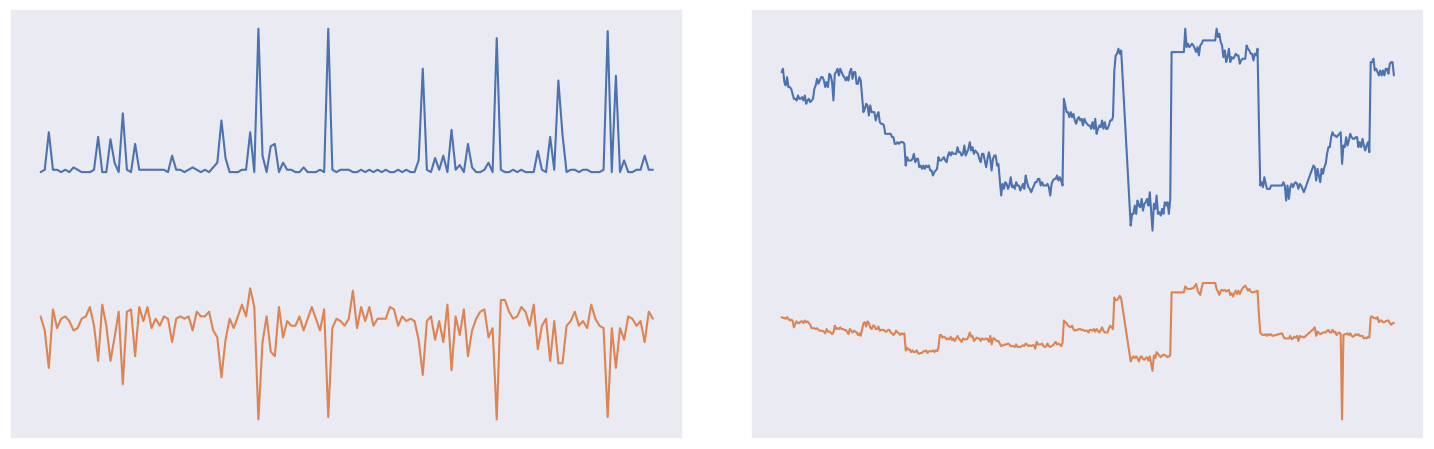
\includegraphics[width=14cm, scale=1]{images/corr}
	\caption{Correlazioni tra features. A sinistra una correlazione negativa, a destra una correlazione positiva.}
	\label{feature-correlazioni}
		
\end{figure}

Utilizzando il coefficiente di Skewness si va a vedere in che direzione portare la anomalia: se verso il basso o verso l'alto. Feature con un right-skew avranno anomalie orientate verso l'alto, left-swek verso il basso mentre se non rientrano in nessuno dei due casi allora si generano anomalie casuali o verso il basso o verso l'alto.

Infine, calcolando l'indice di Kurtosis di definisce la probabilità con cui si sceglie una determinata feature per inserirvi un'anomalia per ogni determinato punto. Un valore di Kurtosis più alto indica una probabilità di anomalie più alta per quella feature, questo per andare a favorire la generazione di anomalie per quelle feature che hanno una deviazione standard molto alta, al contrario di feature più "piatte" che cambiano di rado.


Le tipologie di anomalie sintetiche possono essere iniettate in modo esclusivo, ovvero generando N copie del dataset originario in cui si inseriscono una sola tipologia di anomalia per ognuna; oppure combinandole insieme in un unico dataset. 
Ognuno di questi dataset prodotti viene poi utilizzato per effettuare la valutazione sui modelli generando quindi N ranking differenti. Le performance di ognuno di questi metodi verranno valutate successivamente utilizzando lo F1 Score.

Il flusso di lavoro di questa metrica surrogata può essere riassunto in questi step:
\begin{enumerate}
	\item Training dei modelli sul dataset originario.
	\item Creazione di dataset modificati andando ad iniettare i diversi tipi di anomalie e producendo quindi le pseudo-etichette.
	\item Valutazione dei modelli sui dataset modificati usando le pseudo-etichette come ground truth e F1 Score come metrica di valutazione.
\end{enumerate}


Questa procedura può essere molto efficace ma non è esente da problemi: (1) le anomalie reali non vengono considerate e di conseguenza sono etichettate come pseudo-negative. Questo potrebbe portare a score falsati nel caso i modelli andassero a riconoscere prevalentemente solo le anomalie reali, che però nella fase di valutazione vengono visti come sample negativi. Infine (2) le tipologie di anomalie iniettate possono risultare molto differenti da quelle che sono le reali anomali, rischiando quindi di produrre score molto alti per certi modelli ma che nella realtà funzioneranno particolarmente male sul dataset originario.

\subsubsection{Clustering cohesion}
\textit{Un buon modello riesce a trovare una buona separazione tra i punti normali ed i punti anomali}.
Nel contesto dei modelli non supervisionati, tecniche e metriche di valutazione inerenti al clustering sono molto efficaci quando non si hanno a disposizione le etichette. Misure di coesione tra i cluster prodotti da un modello sono indicatori di quanto quest'ultimo sia riuscito a separare efficacemente i dati.
All'interno del task dell'Anomaly Detection, le anomalie sono punti che si discostano in maniera significativa da un comportamento normale e di conseguenza avranno valori molto diversi rispetto al resto dei punti. Immaginando i punti considerati normali con un unico cluster, ci si aspetta che questi siano ben raggruppati insieme mentre i punti anomali sono sparsi o al più raggruppati in zone poco dense.
\begin{center}
	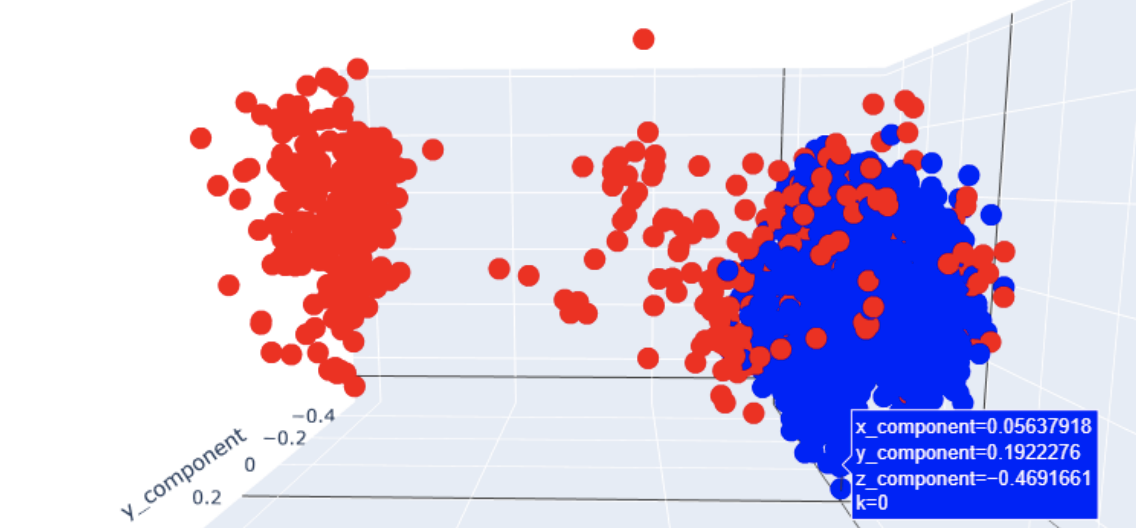
\includegraphics[width=12cm, scale=1]{images/plot-anomalies-normal}
    \captionsetup{type=figure}
	\captionof{figure}{Scatter plot dopo l'Anomaly Detection}
    \label{plot-anomalies-normal}
\end{center}
L'idea alla base di questa metrica surrogata è quindi quella di calcolare la coesione e separazione tra il cluster di punti normali e quello di punti anomali prodotti dalle etichette di un modello di Anomaly Detection. Più alto è questo score, più il modello riesce a separare questi dati e quindi può essere considerato come un buon modello.
La metrica utilizzata è il Silhouette Score, ma non viene calcolata subito dopo aver ottenuto le etichette da un modello. Sono necessari prima alcuni passaggi di processamento del dato.
Immaginiamo di avere un dataset con tre feature per la quale è possibile visualizzare graficamente i punti in un piano tridimensionale. Idealmente i punti considerati normali formano un unico cluster denso, ma la stessa cosa non si può dire per i punti anomali. 
Questi possono essere sparsi per il piano come se fossero rumore oppure possono formare cluster di piccole dimensioni, ma in ogni caso questi punti anomali hanno tutti la stessa etichetta (Figura \ref{plot-anomalies-normal}, in colore rosso).
Il Silhouette Score calcolato assumendo solo etichette di valore 0 o 1 potrebbe risultare falsato proprio per il fatto che i punti sparsi contribuiscono in maniera negativa allora score.

La soluzione adottata è quella di applicare l'algoritmo di DBSCAN sui punti anomali, per formare quindi più cluster da questi e per scartare quei punti che vengono etichettati dall'algoritmo come rumore.
Generalizzando questa idea ad un dataset multidimensionale con numerose feature, è però necessario ridurre la dimensionalità dei dati per evitare il problema del "Curse Of Dimensionality", il quale afferma che in un dataset ad alta dimensionalità, la distanza tra i singoli punti è troppo alta per essere informativa.
Applicando quindi PCA per ridurre le dimensioni a 3 si rende l'applicazione di DBSCAN più efficace. Come parametri per DBSCAN sono stati usati $minsamples=dim \cdot 2$ e per quanto riguarda $eps$ è stato ricavato il valore usando l'Elbow Method. $minsamples$ ed $eps$ sono due parametri fondamentali per la definizione dei punti \textit{core}, \textit{border} e \textit{rumore} durante l'esecuzione di DBSCAN. Ad esempio, un punto viene definito \textit{core} quando contiene altri $minsamples$ punti in un raggio di dimensione $eps$. Solitamente per $minsamples$ si sceglie un valore doppio rispetto al numero di features nel dataset, mentre per $eps$ si usa l'Elbow Method.
Applicando quindi DBSCAN si ottengono i cluster per i punti anomali come mostrato in Figura \ref{plot-dbscan-anomalies}: i punti gialli sono considerati rumore, mentre il restante dei colori sono i cluster di punti anomali.

\begin{center}
	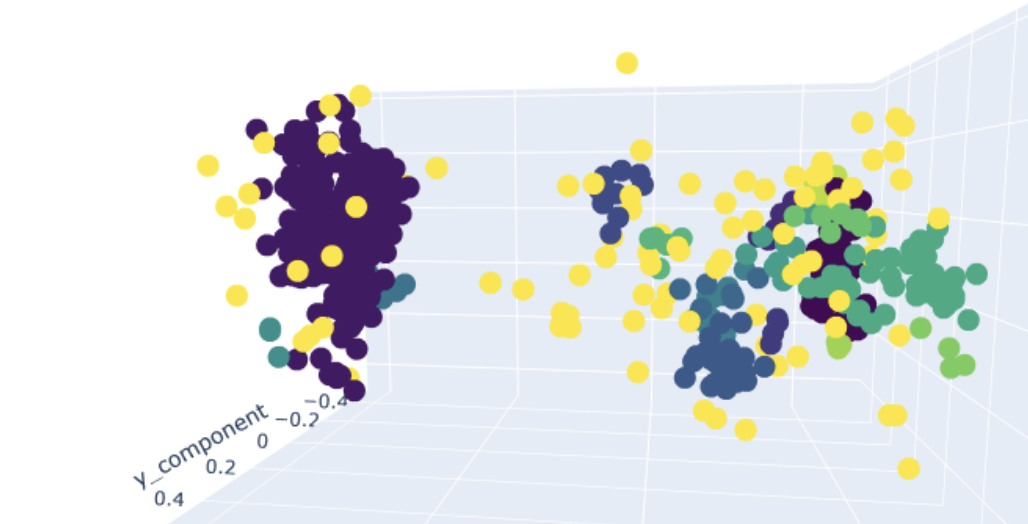
\includegraphics[width=12cm, scale=1]{images/plot-dbscan-anomalies}
    \captionsetup{type=figure}
	\captionof{figure}{Scatter plot dopo DBSCAN sulle anomalie}
    \label{plot-dbscan-anomalies}
\end{center}

Infine viene calcolato il Silhouette Score su questi, tenendo anche in considerazione il cluster di punti normali originario. Questa procedura viene poi applicata su ogni modello per andare a produrre un ranking finale.

Questa metrica surrogata può funzionare particolarmente bene quando una serie temporale è stazionaria e la sua autocorrelazione relativamente bassa, quindi vi è una forte indipendenza tra i punti temporali. Le anomalie a punto così come le anomalie collettive sono identificate con più precisione rispetto alle anomalie contestuali. Infatti, per definizione, i primi due tipi rappresentano punti molto distanti rispetto all'insieme totale, mentre il terzo tipo rappresenta punti distanti rispetto ad un intorno ma che potrebbero essere valutati normali rispetto ad altri intervalli, risultando quindi con più probabilità nel cluster di punti normali.
\subsection{Rank aggregation}
Nel Capitolo \ref{chap:modelselection} è stata fatta una panoramica su Rank Aggregation, vediamo ora quali tecniche sono state implementate. Un'analisi sulle performance di ognuno sarà svolta nelle sezioni successive.
Ognuno di questi metodi riceve in input un set di ranking, ognuno prodotto da una metrica surrogata diversa, ed in output viene generato un'unica classifica finale.
Nel caso delle metriche surrogate Model Centrality e Performance on Injected Synthetic Anomalies, il ranking prodotto si basa sul F1 Score; mentre per Clustering Cohesion sul Silhouette Score.
\subsubsection{Kemeny-Young}
È il metodo di Rank Aggregation ottimale in quanto ottimizza la funzione oggetto come definito nel Capitolo \ref{chap:modelselection}. È un problema NP-Hard ma la complessità temporale, dati solo tre ranking, è sufficientemente bassa da garantirne un utilizzo in tempi brevi. Nella Tabella \ref{kemeny-young}, viene proposto un esempio di Ranking Aggregation con questo metodo. Le prime tre colonne rappresentano le tre classifiche a score prodotte dalle metriche surrogate mentre gli indici di riga corrispondono a quattro modelli.
\begin{table}
	\centering
	\begin{tabular}{|l|l|l|l|l|} 
		\hline
		   & MC  & PAI & CC  & Final Ranking \\ 
		\hline
		M1 & 1   & 0.5 & 0.7 & 0.784         \\ 
		\hline
		M2 & 0.8 & 0.6 & 0.7 & 0.742         \\ 
		\hline
		M3 & 0.6 & 0.7 & 0.8 & 0.930         \\ 
		\hline
		M4 & 0.5 & 0.8 & 0.5 & 0.696         \\
		\hline
	\end{tabular}
 	\caption{\label{kemeny-young}Esempio di aggregazione con Kemeny-Young.}
\end{table}

\subsubsection{Borda}
Le tre classifiche a score prodotte dalle metriche surrogate contenenti gli score per ogni modello vengono convertiti in semplici ranking di posizione in cui il modello con lo score più alto sarà in posizione 1, il secondo con score più alto in posizione 2 e così via. 
Successivamente, per ognuno dei tre ranking di posizione, vengono assegnati dei punteggi ai modelli in base alla posizione in cui si trovano: il modello in ultima posizione riceverà 1 punto, il penultimo 2 punti e così via. Il modello in prima posizione riceverà un numero di punti pari al numero di modelli. 
Dopo aver effettuato questa computazione rispetto a tutte e 3 le classifiche delle metriche surrogate, viene calcolato il punteggio di aggregazione, di ogni modello, come la media dei 3 valori.

\begin{table}
	
	\centering
	\begin{tabular}{|l|l|l|l|l|l|l|l|}
		\hline
		   & MC  & PAI & CC  & B(MC) & B(PAI) & B(CC) & Final Ranking \\ \hline
		M1 & 1   & 0.5 & 0.7 & 4     & 1      & 2.5   & 2.5           \\ \hline
		M2 & 0.8 & 0.6 & 0.7 & 3     & 2      & 2.5   & 2.5           \\ \hline
		M3 & 0.6 & 0.7 & 0.8 & 2     & 3      & 4     & 3             \\ \hline
		M4 & 0.5 & 0.8 & 0.5 & 1     & 4      & 1     & 2             \\ \hline
	\end{tabular}
	\caption{\label{borda}Esempio di aggregazione con Borda.}
\end{table}


Nella Tabella \ref{borda}, viene riproposto l'esempio precedente ma utilizzando Borda. Le prime 3 colonne sono gli stessi score delle metriche surrogate, invece le seconde 3 colonne rappresentano i punteggi che ogni modello ha ricevuto secondo il metodo Borda. Infine, l'ultima colonna rappresenta il punteggio medio. Lo score più alto è stato ottenuto dal modello M3, risultando poi primo nella classifica finale.
\subsubsection{Robust borda}
È una variazione del metodo Borda in cui viene scelto un parametro $k$ e per ogni ranking viene assegnato il punteggio solamente ai primi $k$ modelli mentre i restanti vengono considerati come se fossero tutti in ultima posizione, ricevendo così il punteggio minimo, ovvero 1. Questo metodo cerca di migliorare le performance del metodo Borda andando a penalizzare i modelli che finiscono in ultima posizione in un determinato ranking. 

\begin{table}
	
	\centering
	\begin{tabular}{|l|l|l|l|l|l|l|l|}
		\hline
		   & MC  & PAI & CC  & rB(MC) & rB(PAI) & rB(CC) & Final Ranking \\ \hline
		M1 & 1   & 0.5 & 0.7 & 4      & 1       & 2.5    & 2.5           \\ \hline
		M2 & 0.8 & 0.6 & 0.7 & 3      & 1       & 2.5    & 2.16          \\ \hline
		M3 & 0.6 & 0.7 & 0.8 & 1      & 3       & 4      & 2.66          \\ \hline
		M4 & 0.5 & 0.8 & 0.5 & 1      & 4       & 1      & 2             \\ \hline
	\end{tabular}
	\caption{\label{rborda}Esempio di aggregazione con Robust Borda.}
\end{table}

Continuando con lo stesso esempio in Tabella \ref{rborda} e assumendo il parametro \(k=2\), i punteggi di Robust Borda per Model Centrality e Performance on Injected Synthetic Anomalies cambiano rispettivamente per i modelli M3 e M2 che ricevono entrambi il punteggio minimo, ovvero 1, nonostante non siano ultimi e andando a penalizzare il loro score finale. M3 è sempre quello con score più alto ma in questo caso la differenza con M1 si è fatta più piccola.

\subsubsection{AVG score}
Questo metodo è il più semplice dei 3 in quanto viene semplicemente fatta una media degli score dei 3 ranking per ogni modello, per poi ordinare in ordine decrescente e quindi ottenere un ranking finale.
Utilizzando questo metodo e sempre considerando gli stessi score degli esempi precedenti, in Tabella \ref{score} si può notare come questa volta il modello migliore sia M1 e non più M3.

\begin{table}
	
	\centering
	\begin{tabular}{|l|l|l|l|l|}
		\hline
		   & MC  & PAI & CC  & Final Ranking(AVG) \\ \hline
		M1 & 1   & 0.5 & 0.7 & 0.73               \\ \hline
		M2 & 0.8 & 0.6 & 0.7 & 0.7                \\ \hline
		M3 & 0.6 & 0.7 & 0.8 & 0.7                \\ \hline
		M4 & 0.5 & 0.8 & 0.5 & 0.6                \\ \hline
	\end{tabular}
	\caption{\label{score}Esempio di aggregazione con Score.}
\end{table}


Chiaramente il processo di Ranking Aggregation aggiunge complessità e variabilità al processo di Model Selection, un'analisi sui risultati di ognuno dei metodi appena proposti è riportata nella sezione successiva. In generale però, il metodo ottimale di Kemeny-Young risulterà il migliore e sarà poi utilizzato su SKF.


\subsection{Valutazione}
Per confrontare i risultati ottenuti dalle metriche surrogate si è deciso di adottare le misure di correlazione tra le classifiche a score o le classiche di posizione rispetto a quelle ottenute usando le etichette. Per queste ultime, la metrica scelta è F1 Score.
Quindi, utilizzando l'algoritmo di Model Selection, vengono prodotti dei ranking contenenti gli score di ogni modello per ogni metrica surrogata più un ranking per ogni tecnica di aggregazione. Confrontare ogni singola metrica surrogata e non soltanto l'aggregazione finale permette di avere una panoramica completa delle performance di ognuno.
Questi vengono confrontati con il ranking prodotto da una valutazione usando le etichette ground-truth dei dataset di benchmark con la metrica F1 Score.
Gli algoritmi di calcolo per il coefficiente di correlazione sono Kendall e Spearman per il Rank Correlation e Pearson per lo Score Correlation. Tutti e tre i coefficienti hanno un range compreso tra $[-1,1]$ dove un coefficiente di -1 indica una correlazione negativa, 0 nessuna correlazione mentre 1 una correlazione positiva. 
Dato che questi coefficienti hanno caratteristiche diverse è necessario andare a trattare separatamente il calcolo:
\begin{itemize}
	\item Rank Correlation: Kendall e Spearman utilizzando delle classifiche di posizione per calcolare il coefficiente di correlazione. Questo vuol dire che bisogna andare a trasformare tutti i ranking con gli score in ranking di posizione in cui il modello con score più alto avrà come posizione 1 ed i restanti a seguire.
	\item Score Correlation: Pearson invece necessita di valori continui, di conseguenza per questo coefficiente non si effettua nessuna trasformazione e si usano i ranking con gli score così come sono prodotti dal Model Selection.
\end{itemize}

 

\newpage
\section{Risultati di benchmark}
\subsection{Dataset}
I dataset trattati sono diversi sia per struttura ma anche per tipologia: verranno dapprima introdotti semplici dataset multidimensionali a punto per poi passare a serie temporali multivariate. 

\subsubsection{ODDS}
Outlier Detection DataSets\footnote{ODDS: http://odds.cs.stonybrook.edu/} è una collezione di dataset per l'Outlier Detection. Questo archivio è in continuo sviluppo dal 2016 da parte di numerosi ricercatori e comprende dataset di vari domini, dimensione, numero di features e percentuale di anomalie. 
I dataset sono di tipo multi-dimensionale a punto, quindi senza una componente temporale associata.
La Tabella \ref{odds} elenca tutti i dataset di ODDS utilizzati.

\begin{table}
	
	\centering
	\begin{tabular}{|l|l|l|l|l|}
		\hline
		\textbf{Dataset} & \textbf{\#punti} & \textbf{\#dim} & \textbf{\#anomalie(\%)} & \textbf{dominio} \\ \hline
		annthyroid       & 7200              & 6              & 534 (7.42\%)            & Healthcare      \\ \hline
		cardio           & 1831              & 21             & 176 (9.61\%)            & Healthcare      \\ \hline
		cover            & 286048            & 10             & 2747 (0.96\%)           & Botany          \\ \hline
		donors           & 619326            & 10             & 36710 (5.93\%)          & Sociology       \\ \hline
		mammography      & 11183             & 6              & 260 (2.32\%)            & Healthcare      \\ \hline
		PageBlocks       & 5393              & 10             & 510 (9.46\%)            & Document        \\ \hline
		satimage-2       & 5803              & 36             & 71 (1.22\%)             & Astronautics    \\ \hline
		shuttle          & 49097             & 9              & 3511 (7.15\%)           & Astronautics    \\ \hline
		thyroid          & 3772              & 6              & 93 (2.47\%)             & Healthcare      \\ \hline
		vowels           & 1456              & 12             & 50 (3.43\%)             & Linguistics     \\ \hline
		Waveform         & 3443              & 21             & 100 (2.9\%)             & Physics         \\ \hline
		Wilt             & 4819              & 5              & 257 (5.33\%)            & Botany          \\ \hline
	\end{tabular}
	\caption{\label{odds}Dataset ODDS}
\end{table}

Per questi dataset si è deciso di adottare uno split train/test costituito da 66\% per il train e 33\% per il test. I dataset di train contengono al loro interno anche una percentuale di anomalie. Potrebbe non essere la situazione ideale in quanto è consigliato per i modelli non supervisionati di essere allenati e quindi apprendere da dati il più puliti possibili. Ma è la situazione più realistica in quanto nella realtà la presenza di etichette non è sempre garantita.  

\subsubsection{SMD}
Server Machine Dataset\footnote{SMD: https://github.com/NetManAIOps/OmniAnomaly} è un dataset proveniente da una compagnia Internet, consiste in serie temporali multivariate della durata di 5 settimane in cui ogni osservazione è equamente distribuita da una frequenza di 1 minuto. SMD contiene tre gruppi di macchinari (denotati SMD-1, SMD-2 e SMD-3 rispettivamente) per un totale di 28 macchinari, ed ognuno di questi ha 38 features. Sono presenti approssimativamente 28000 time step, sia per i dati di train che quelli di test. 
La percentuale di anomalie al suo interno si attesta intorno al 4.16\% e si trovano tutte nell'ultima metà dei dati (ultime due settimane circa). Per questi dataset, la prima metà dei dati viene quindi usata per il training dei modelli mentre il restante per la predizione.
Le anomalie sono raggruppate in intervalli di varia lunghezza e sono anomalie a punto.
\begin{table}
\centering
\caption{\label{smd}Caratteristiche di SMD}
\begin{tabular}{|c|c|} 
\hline
\textbf{Proprietà} & \textbf{Valore}                              \\ 
\hline
\#dataset     & 28                                           \\ 
\hline
\#dim     & 38                                           \\ 
\hline
frequenza         & 1/minuto                                  
                                   \\ 
\hline
\%anomalie & 4.16                                         \\ 
\hline
misure              & CPU load, network usage, memory usage, etc.  \\
\hline
\end{tabular}
\end{table}


\subsection{Modelli}
Per una valutazione più completa si è deciso di utilizzare un alto numero di modelli ognuno con caratteristiche e proprietà differenti. Algoritmi di Machine Learning basati sulla distanza, probabilistici o lineari; ma anche Neural Network come Auto Encoders o LSTM. La Tabella \ref{admodels} è comprensiva di tutti i modelli considerati.

Gli algoritmi di Machine Learning considerano i sample in maniera indipendente, mentre quelli a rete neurale considerano una finestra temporale per andare a fare sia training che prediction, risultando quindi time-aware, ovvero tengono in considerazione l'aspetto temporale dei dati. Il valore di questa finestra temporale viene passato come parametro e valorizzato manualmente.
Questo implica che i metodi di Machine Learning non riusciranno a predire le anomalie contestuali, proprio per il fatto che non modellano l'informazione di contesto. 
Sui dataset di benchmark questo non è un problema, in quanto semplici dataset multidimensionali o con anomalie a punto; e per SKF il discorso è simile: la bassa frequenza di registrazione (1/10 minuti) e la stazionarietà delle serie temporali rende difficile capire se anomalie contestuali possano essere presenti o meno. Per questo motivo si procederà con un'ampia gamma di modelli di Machine Learning.


Come definito nel Capitolo \ref{chap:modelselection}, questi modelli producono in output uno score per ogni sample dove uno score più alto indica una probabilità maggiore che quel sample sia anomalo. Questi score vengono trasformati in etichette \(\in \{0,1\}\) andando a specificare un fattore di contaminazione $c$, ovvero la percentuale di punti anomali. I top $c\%$ dei sample con score più alto saranno etichettati come anomali. 

Ognuno di questi modelli è stato allenato utilizzando sia i valori predefiniti per gli iperparametri, sia variazioni di questi. 
Per la maggior parte degli algoritmi sono state considerate in media 3 versioni con parametri differenti, alcuni invece sono algoritmi parameter-free e quindi viene considerata solamente una versione, portando il totale dei modelli a 70.
La scelta dei valori modificati agli iperparametri è stata fatta manualmente a priori, senza conoscere le performance del modello. Il focus della tesi si mantiene sul Model Selection, mentre un approfondimento sul tuning dei parametri può essere lasciato a sviluppi futuri.
I modelli di Deep Learning contengono un parametro chiamato \textit{window\_len}, che, come discusso prima, serve per andare a specificare la finestra temporale che il modello deve considerare durante l'esecuzione di train e prediction. Per questo parametro sono stati scelti i valori 1 e 48, andando così a creare due modelli per tipologia di algoritmo. 
Un valore di \textit{window\_len} a 1 significa che verrà trattato ogni sample in maniera indipendente, così come fanno i classici metodi di Machine Learning; mentre un valore di 48 consente ai modelli di andare a utilizzare l'informazione temporale per il training e predizione.

Il fattore di contaminazione passato ad ogni modello corrisponde esattamente alla percentuale di anomalie presenti in ogni dataset di benchmark. Questa situazione è ottimale in quanto il numero di punti anomali trovati dai modelli coincide con il numero di anomalie reali. Ovviamente non è possibile replicare questo anche sul dataset di SKF in quanto qualsiasi informazione sulle anomalie non è presente. Per risolvere questo problema si utilizzerà un metodo di Thresholding chiamato ${\gamma}GMM$, come introdotto nel Capitolo \ref{chap:methods}, che stima il fattore di contaminazione. Un fattore di contaminazione stimato erroneamente porta ovviamente a degradare le performance del Model Selection. Così come per la variazione degli iperparametri, in sviluppi futuri potrebbe risultare utile un'analisi più approfondita andando anche a testare l'algoritmo con diversi valori per il fattore di contaminazione.



\begin{table}
\centering
\caption{\label{admodels}Algoritmi di Anomaly Detection}
\resizebox{\linewidth}{!}{%
\begin{tabular}{|l|l|l|} 
\hline
\textbf{Model} & \textbf{Type}     & \textbf{Algorithm}                                                      \\ 
\hline
ECOD           & Probabilistic     & Outlier Detection Using Empirical Cumulative Distribution Functions     \\ 
\hline
COPOD          & Probabilistic     & Copula-Based Outlier Detection                                          \\ 
\hline
ABOD           & Probabilistic     & Angle-Based Outlier Detection                                           \\ 
\hline
SOS            & Probabilistic     & Stochastic Outlier Selection                                            \\ 
\hline
KDE            & Probabilistic     & Outlier Detection with Kernel Density Functions                         \\ 
\hline
Sampling       & Probabilistic     & Rapid distance-based outlier detection via sampling                     \\ 
\hline
GMM            & Probabilistic     & Probabilistic Mixture Modeling for Outlier Analysis                     \\ 
\hline
PCA            & Linear Model      & Principal Component Analysis                                            \\ 
\hline
KPCA           & Linear Model      & Kernel Principal Component Analysis                                     \\ 
\hline
MCD            & Linear Model      & Minimum Covariance Determinant                                          \\ 
\hline
OCSVM          & Non Linear Model      & One-Class Support Vector Machines                                       \\ 
\hline
LMDD           & Linear Model      & Deviation-based Outlier Detection                                       \\ 
\hline
AutoRegressive & Linear Model      & Autoregressive modeling that uses past data to predict future behavior  \\ 
\hline
LOF            & Proximity-Based   & Local Outlier Factor                                                    \\ 
\hline
COF            & Proximity-Based   & Connectivity-Based Outlier Factor                                       \\ 
\hline
CBLOF          & Proximity-Based   & Clustering-Based Local Outlier Factor                                   \\ 
\hline
HBOS           & Proximity-Based   & Histogram-based Outlier Score                                           \\ 
\hline
KNN            & Proximity-Based   & k Nearest Neighbors                                                     \\ 
\hline
SOD            & Proximity-Based   & Subspace Outlier Detection                                              \\ 
\hline
ROD            & Proximity-Based   & Rotation-based Outlier Detection                                        \\ 
\hline
IForest        & Outlier Ensembles & Isolation Forest                                                        \\ 
\hline
INNE           & Outlier Ensembles & Isolation-based Anomaly Detection Using Nearest-Neighbor Ensembles      \\ 
\hline
FB             & Outlier Ensembles & Feature Bagging                                                         \\ 
\hline
AutoEncoder    & Neural Networks   & Fully connected AutoEncoder                                             \\ 
\hline
VAE            & Neural Networks   & Variational AutoEncoder                                                 \\ 
\hline
DeepSVDD       & Neural Networks   & Deep One-Class Classification                                           \\ 
\hline
ALAD           & Neural Networks   & Bi-Directional GAN                                                      \\ 
\hline
AnoGAN         & Neural Networks   & Adversarially learned anomaly detection                                 \\ 
\hline
DeepLog        & Neural Networks   & LSTM based neural-network that models system logs                       \\ 
\hline
Telemanom      & Neural Networks   & LSTM to detect anomalies in multivariate time series data               \\ 
\hline
LSTM           & Neural Networks   & LSTM based neural-network                                               \\ 
\hline
LUNAR          & Graph-based       & Unifying Local Outlier Detection Methods via Graph Neural Networks      \\
\hline
\end{tabular}
}
\end{table}







\subsection{Risultati}
I risultati saranno mostrati in formato tabulare rispetto a tutti i dataset di benchmark, insieme ai valori di media e deviazione standard, sia per le singole metriche surrogate che per tutti i metodi di Rank Aggregation.
I valori fanno riferimento agli indici di correlazione dei ranking prodotti rispetto alla classifica prodotta usando le etichette e F1 Score.


\subsubsection{Model centrality}
Questa metrica surrogata si basa sul concetto di Model Centrality andando a favorire quei modelli che producono output comparabili alla maggior parte degli altri modelli. Delle quattro tecniche proposte, Round Robin è quella che generalmente si comporta meglio. In Tabella \ref{mc-results} possiamo vedere come gli indici di correlazione favoriscano questa tecnica.
Majority Vote e Sampling seguono con punteggi molto simili, sia per le performance medie che per deviazione standard. Il metodo AVG Score fatica a trovare correlazione con il ranking supervisionato. 
Generalmente però, la metrica funziona discretamente bene tranne qualche dataset specifico come Machine-3-10.  Nelle Figure \ref{model-centrality-plot-bad} e \ref{model-centrality-plot-good} sono mostrati dei scatter plot in cui i punti rappresentano i modelli e dove questi si posizionano in uno spazio bidimensionale. La posizione viene calcolata riducendo a due dimensioni l'output delle predizioni di ogni modello.  Nella figura della Machine-3-10 possiamo notare come i punti sono sparsi lungo tutto il piano rendendo difficile alla metrica surrogata riuscire a trovare una definizione per modello centrale.
Per Machine-1-4, invece, le performance di correlazione sono migliori e possiamo anche notare come la maggior parte dei punti risieda nel cluster formatosi sulla sinistra. Questo permette di spostare la centralità di un modello verso quella zona ed è anche altamente probabile che il miglior modello si trovi li, migliorando di conseguenza la correlazione tra il ranking di Model Centrality ed il ranking supervisionato.
Come si vedrà più avanti, questa metrica è la più stabile delle tre, ovvero che le performance variano relativamente meno rispetto ad ogni dataset. Motivo di ciò è che questa metrica non lavora direttamente sui dati del dataset ma sugli output dei modelli ed è quindi suscettibile alla lista di modelli che si passa in input al Model Selection. Se non si ha conoscenza su quali modelli potrebbero funzionare meglio è dunque consigliato utilizzare un numero di modelli che abbiano caratteristiche diverse sufficientemente alto in modo da non rischiare di condizionare la centralità orientandola verso quei modelli meno preformanti.
D'altro canto, però, questo è anche il suo punto di forza perché riesce a sfruttare nel modo migliore l'informazione proveniente da ciascuno dei modelli, risultando, in questi esperimenti, migliore delle altre due metriche surrogate.

\begin{figure}[]
	\centering
	\begin{minipage}[b]{0.45\textwidth}
		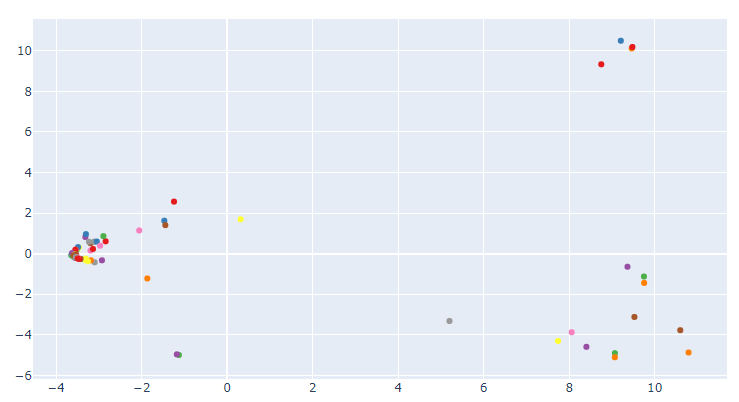
\includegraphics[width=\textwidth]{images/model_centrality_good2-8_2}
		\caption{Machine-1-4}
		\label{model-centrality-plot-good}
	\end{minipage}
	\begin{minipage}[b]{0.45\textwidth}
		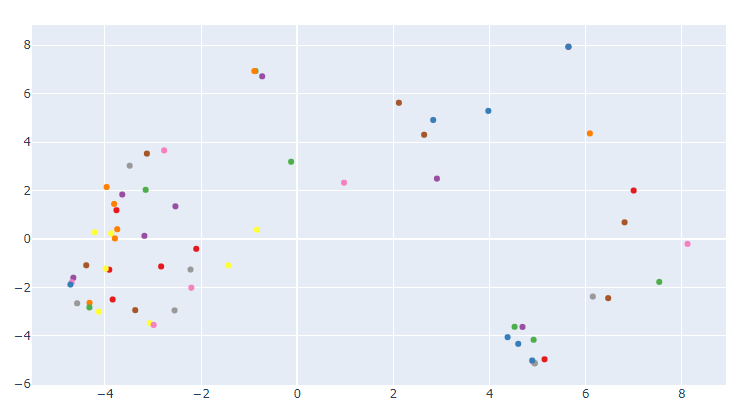
\includegraphics[width=\textwidth]{images/model_centrality_bad3-10_2}
		\caption{Machine-3-10}
		\label{model-centrality-plot-bad}
	\end{minipage}
\end{figure}

\begin{table}[]
	\caption{\label{mc-results}Risultati di correlazione per Model Centrality}
	\resizebox{\linewidth}{!}{%
		\begin{tabular}{|l||l|l|l|l||l|l|l|l||l|l|l|l|} 
			\hline
			Dataset           & \multicolumn{4}{c||}{SCORE CORRELATION} & \multicolumn{8}{c|}{RANK CORRELATION}                            \\ 
			\hline
			\multirow{2}{*}{} & \multicolumn{4}{c||}{PEARSON}           & \multicolumn{4}{c||}{KENDALL}  & \multicolumn{4}{c|}{SPEARMAN}   \\ 
			\cline{2-13}
			                & mv     & rr    & samp  & score  & mv    & rr    & samp  & score & mv    & rr           & samp   & score \\ 
			\hline
			2\_annthyroid   & 0.823  & 0.837 & 0.836 & 0.773  & 0.584 & 0.581 & 0.605 & 0.584 & 0.739 & 0.735        & 0.753  & 0.671 \\ 
			\hline
			6\_cardio       & 0.807  & 0.787 & 0.787 & 0.654  & 0.612 & 0.563 & 0.564 & 0.565 & 0.746 & 0.715        & 0.718  & 0.626 \\ 
			\hline
			11\_donors      & 0.514  & 0.529 & 0.526 & 0.423  & 0.541 & 0.511 & 0.529 & 0.475 & 0.665 & 0.650        & 0.670  & 0.559 \\ 
			\hline
			20\_letter      & 0.559  & 0.631 & 0.763 & 0.669  & 0.473 & 0.499 & 0.692 & 0.536 & 0.565 & 0.608        & 0.840  & 0.642 \\ 
			\hline
			23\_mammography & 0.795  & 0.829 & 0.801 & 0.607  & 0.694 & 0.722 & 0.649 & 0.439 & 0.834 & 0.821        & 0.809  & 0.561 \\ 
			\hline
			27\_PageBlocks  & 0.917  & 0.911 & 0.909 & 0.832  & 0.698 & 0.677 & 0.646 & 0.550 & 0.812 & 0.849        & 0.818  & 0.717 \\ 
			\hline
			31\_satimage-2  & 0.759  & 0.855 & 0.644 & 0.553  & 0.641 & 0.865 & 0.514 & 0.440 & 0.793 & 0.970        & 0.581  & 0.462 \\ 
			\hline
			32\_shuttle     & 0.489  & 0.846 & 0.827 & 0.661  & 0.446 & 0.774 & 0.770 & 0.565 & 0.456 & 0.894        & 0.890  & 0.728 \\ 
			\hline
			38\_thyroid     & 0.719  & 0.761 & 0.701 & 0.709  & 0.538 & 0.563 & 0.508 & 0.546 & 0.667 & 0.700        & 0.632  & 0.683 \\ 
			\hline
			40\_vowels      & 0.735  & 0.760 & 0.670 & 0.612  & 0.637 & 0.642 & 0.573 & 0.463 & 0.779 & 0.806        & 0.721  & 0.582 \\ 
			\hline
			41\_Waveform    & 0.428  & 0.464 & 0.440 & 0.481  & 0.466 & 0.582 & 0.569 & 0.423 & 0.572 & 0.709        & 0.647  & 0.541 \\ 
			\hline
			machine-1-1     & 0.561  & 0.582 & 0.641 & 0.556  & 0.458 & 0.458 & 0.499 & 0.468 & 0.558 & 0.572        & 0.607  & 0.595 \\ 
			\hline
			machine-1-2     & 0.842  & 0.877 & 0.866 & 0.771  & 0.633 & 0.732 & 0.723 & 0.570 & 0.834 & 0.839        & 0.836  & 0.738 \\ 
			\hline
			machine-1-3     & 0.949  & 0.836 & 0.828 & 0.480  & 0.855 & 0.633 & 0.645 & 0.437 & 0.934 & 0.841        & 0.826  & 0.428 \\ 
			\hline
			machine-1-4     & 0.966  & 0.949 & 0.917 & 0.576  & 0.835 & 0.706 & 0.711 & 0.412 & 0.927 & 0.842        & 0.840  & 0.553 \\ 
			\hline
			machine-1-5     & 0.441  & 0.494 & 0.465 & 0.353  & 0.458 & 0.477 & 0.456 & 0.432 & 0.587 & 0.514        & 0.584  & 0.419 \\ 
			\hline
			machine-1-6     & 0.588  & 0.551 & 0.576 & 0.585  & 0.550 & 0.527 & 0.528 & 0.521 & 0.621 & 0.582        & 0.578  & 0.601 \\ 
			\hline
			machine-1-7     & 0.630  & 0.596 & 0.626 & 0.597  & 0.546 & 0.491 & 0.543 & 0.467 & 0.693 & 0.636        & 0.680  & 0.593 \\ 
			\hline
			machine-1-8     & 0.594  & 0.563 & 0.553 & 0.628  & 0.494 & 0.421 & 0.492 & 0.406 & 0.590 & 0.433        & 0.514  & 0.553 \\ 
			\hline
			machine-2-1     & 0.791  & 0.838 & 0.847 & 0.566  & 0.561 & 0.595 & 0.563 & 0.465 & 0.653 & 0.687        & 0.690  & 0.535 \\ 
			\hline
			machine-2-2     & 0.822  & 0.824 & 0.827 & 0.683  & 0.608 & 0.594 & 0.565 & 0.503 & 0.794 & 0.770        & 0.739  & 0.601 \\ 
			\hline
			machine-2-3     & 0.825  & 0.827 & 0.834 & 0.606  & 0.648 & 0.610 & 0.638 & 0.444 & 0.819 & 0.771        & 0.798  & 0.546 \\ 
			\hline
			machine-2-4     & 0.307  & 0.309 & 0.285 & 0.192  & 0.357 & 0.348 & 0.301 & 0.389 & 0.411 & 0.369        & 0.310  & 0.317 \\ 
			\hline
			machine-2-5     & 0.044  & 0.133 & 0.126 & 0.136  & 0.332 & 0.379 & 0.351 & 0.383 & 0.380 & 0.356        & 0.326  & 0.325 \\ 
			\hline
			machine-2-6     & 0.896  & 0.872 & 0.893 & 0.568  & 0.703 & 0.648 & 0.679 & 0.511 & 0.816 & 0.823        & 0.801  & 0.594 \\ 
			\hline
			machine-2-7     & 0.882  & 0.885 & 0.839 & 0.820  & 0.683 & 0.718 & 0.662 & 0.648 & 0.823 & 0.848        & 0.806  & 0.806 \\ 
			\hline
			machine-2-8     & 0.991  & 0.989 & 0.983 & 0.803  & 0.861 & 0.876 & 0.847 & 0.532 & 0.961 & 0.966        & 0.950  & 0.627 \\ 
			\hline
			machine-2-9     & 0.627  & 0.649 & 0.664 & 0.420  & 0.492 & 0.472 & 0.480 & 0.414 & 0.597 & 0.569        & 0.571  & 0.409 \\ 
			\hline
			machine-3-1     & 0.458  & 0.467 & 0.532 & 0.485  & 0.431 & 0.444 & 0.453 & 0.381 & 0.483 & 0.504        & 0.591  & 0.427 \\ 
			\hline
			machine-3-2     & 0.613  & 0.646 & 0.670 & 0.727  & 0.595 & 0.595 & 0.627 & 0.638 & 0.753 & 0.761        & 0.785  & 0.814 \\ 
			\hline
			machine-3-3     & 0.345  & 0.379 & 0.365 & 0.388  & 0.420 & 0.384 & 0.364 & 0.468 & 0.475 & 0.451        & 0.434  & 0.454 \\ 
			\hline
			machine-3-4     & 0.158  & 0.168 & 0.224 & -0.036 & 0.271 & 0.241 & 0.293 & 0.095 & 0.331 & 0.281        & 0.334  & 0.154 \\ 
			\hline
			machine-3-5     & 0.857  & 0.871 & 0.864 & 0.521  & 0.699 & 0.774 & 0.759 & 0.470 & 0.817 & 0.880        & 0.870  & 0.523 \\ 
			\hline
			machine-3-6     & 0.338  & 0.311 & 0.292 & 0.069  & 0.393 & 0.305 & 0.391 & 0.365 & 0.463 & 0.379        & 0.351  & 0.312 \\ 
			\hline
			machine-3-7     & 0.308  & 0.361 & 0.321 & 0.299  & 0.469 & 0.447 & 0.452 & 0.365 & 0.493 & 0.464        & 0.474  & 0.443 \\ 
			\hline
			machine-3-8     & 0.648  & 0.651 & 0.700 & 0.471  & 0.579 & 0.547 & 0.590 & 0.412 & 0.696 & 0.682        & 0.727  & 0.570 \\ 
			\hline
			machine-3-9     & 0.580  & 0.477 & 0.496 & 0.431  & 0.665 & 0.589 & 0.588 & 0.463 & 0.833 & 0.710        & 0.719  & 0.595 \\ 
			\hline
			machine-3-10    & -0.009 & 0.015 & 0.116 & 0.010  & 0.269 & 0.288 & 0.300 & 0.210 & 0.348 & 0.322        & 0.324  & 0.272 \\ 
			\hline
			machine-3-11    & 0.837  & 0.626 & 0.560 & 0.372  & 0.640 & 0.465 & 0.332 & 0.348 & 0.813 & 0.470        & 0.401  & 0.315 \\ 
			\hline
			AVG             & 0.627  & 0.640 & 0.636 & 0.514  & 0.560 & 0.558 & 0.550 & 0.457 & 0.670 & 0.661        & 0.655  & 0.536 \\ 
			\hline
			STD             & 0.25   & 0.24  & 0.229 & 0.214  & 0.142 & 0.149 & 0.135 & 0.102 & 0.169 & 0.186        & 0.177  & 0.146 \\
			\hline
		\end{tabular}
	}
\end{table}

\newpage
\subsubsection{Performance on injected synthetic anomalies}
Passando alla metrica surrogata usante le pseudo-etichette dopo l'iniezione di anomalie, le tipologie di anomalia iniettate sono Spike, Scale, Growing e Mix dove Mix rappresenta i dataset a cui sono state iniettate tutte e tre le tipologie di anomalie trattate a inizio capitolo. Possiamo notare in Tabella \ref{pai-results} come generalmente le performance siano inferiori rispetto alla tecnica del Model Centrality. I motivi di ciò possono essere molteplici: primo tra tutti il fatto che questa metrica non utilizza in nessun modo l'informazione proveniente dagli altri modelli, questi vengono infatti considerati in maniera indipendente e separata. Altre motivazioni possono ricondursi agli aspetti negativi introdotti precedentemente che riguardano questo approccio: (1) come le anomalie vengono generate e (2) le anomalie reali vengano ignorate.

Il primo punto non è banale, avere una conoscenza forte dal dataset di riferimento permette di creare anomalie che possano risultare realistiche ma spesso ciò non è possibile. Attraverso metodi statistici si possono estrarre informazioni riguardanti l'andamento e l'evoluzione dei dati ma spesso le anomalie non seguono un pattern preciso rendendo quindi la generazione di queste un problema non triviale. 
Vediamo ora alcuni esempi di come le performance variano in base al dataset ed al tipo di anomalia iniettata. Le performance dell'anomalia Spike sul dataset Shuttle sono buone e a conferma di ciò si può vedere in Figura \ref{shuttle-inj} come le anomalie prevalenti siano proprio di tipo Spike.
Al contrario, Machine-3-5 ha performance basse per quanto riguarda Growing, Spike e Mix, ma ottiene un punteggio di 0.84 su Scale. La Figura \ref{machine-3-5-inj} mostra come i punti anomali reali abbiano intervalli con valori scalati verso l'alto. Infine, Machine-2-8 è quello con le performance Mix più alte, a riprova del fatto che nella Figura \ref{machine-2-8-inj} si possono notare sia spike, sia intervalli anomali e sia valori crescenti nel tempo.
Il secondo punto trattato può impattare negativamente i risultati in quanto è possibile che il modello vada a etichettare le anomalie reali come positive, nonostante abbiano delle etichette pseudo-negative. Una soluzione a questo problema potrebbe essere quello di ricercare una finestra temporale del dataset che sia il più pulita possibile dalle anomalie per poi andare ad effettuare le iniezioni di anomalia ed infine la valutazione su quell'intervallo.
Delle quattro tipologie di anomalie iniettate (compreso Mix), ci sono tre metodi con performance simili: Spike, Scale e Mix; mentre Growing è generalmente meno performante.
\begin{figure}[htp]% [H] is so declass\'e!
	\centering
	\begin{minipage}{0.5\textwidth}
		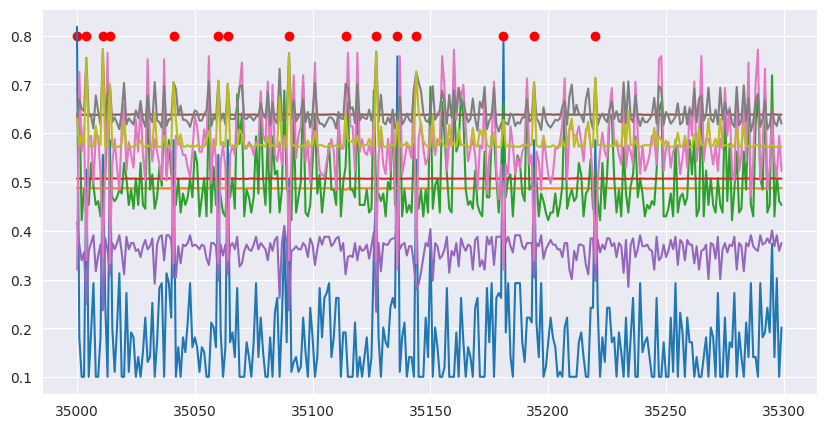
\includegraphics[width=\textwidth]{images/shuttle_good_inj_spike.png}
		\caption{Shuttle}
		\label{shuttle-inj}
	\end{minipage}\hfill
	\begin{minipage}{0.5\textwidth}
		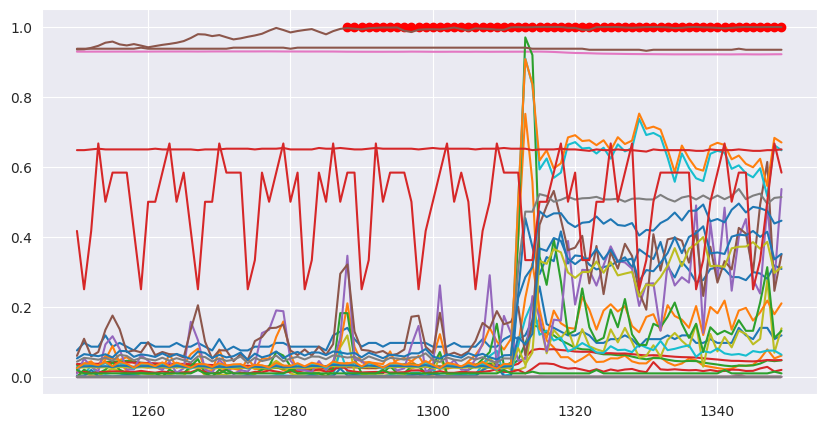
\includegraphics[width=\textwidth]{images/machine-3-5_bad_inj_good_scale.png}
		\caption{Machine-3-5}
		\label{machine-3-5-inj}
	\end{minipage}\par
	\vskip\floatsep% normal separation between figures
	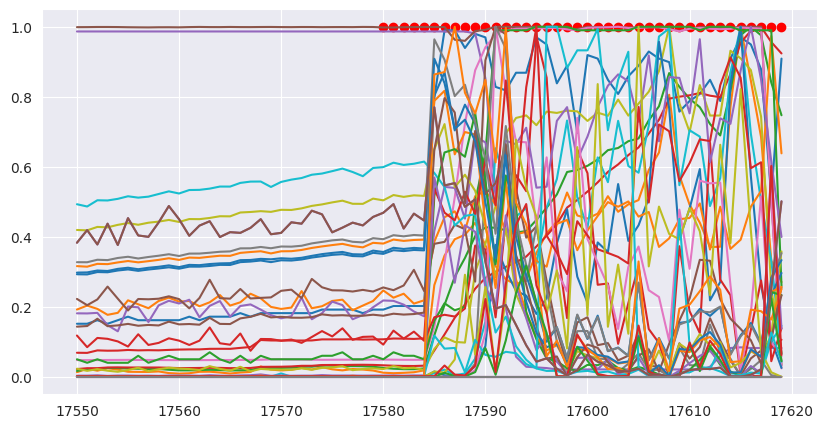
\includegraphics[width=0.5\textwidth]{images/machine-2-8_good_inj_mix.png}
	\caption{Machine-2-8}
	\label{machine-2-8-inj}
\end{figure}

\begin{table}[]
	\caption{\label{pai-results}Risultati di correlazione per Performance on Injected Synthetic Anomalies}
	\resizebox{\linewidth}{!}{%
		\begin{tabular}{|l||l|l|l|l||l|l|l|l||l|l|l|l|} 
			\hline
			Dataset           & \multicolumn{4}{c||}{SCORE CORRELATION} & \multicolumn{8}{c|}{RANK CORRELATION}                            \\ 
			\hline
			\multirow{2}{*}{} & \multicolumn{4}{c||}{PEARSON}           & \multicolumn{4}{c||}{KENDALL}  & \multicolumn{4}{c|}{SPEARMAN}   \\ 
			\cline{2-13}
			                & growing & spike & scale & mix   & growing & spike & scale & mix   & growing & spike        & scale & mix   \\ 
			\hline
			2\_annthyroid   & 0.111  & 0.272 & 0.331 & 0.196 & 0.267  & 0.440 & 0.465 & 0.408 & 0.281  & 0.487        & 0.414 & 0.457 \\ 
			\hline
			6\_cardio       & 0.269  & 0.575 & 0.554 & 0.381 & 0.129  & 0.337 & 0.431 & 0.356 & 0.176  & 0.406        & 0.416 & 0.396 \\ 
			\hline
			11\_donors      & 0.331  & 0.391 & 0.316 & 0.303 & 0.472  & 0.422 & 0.442 & 0.443 & 0.491  & 0.550        & 0.575 & 0.573 \\ 
			\hline
			20\_letter      & 0.457  & 0.577 & 0.811 & 0.560 & 0.489  & 0.607 & 0.718 & 0.527 & 0.563  & 0.742        & 0.805 & 0.597 \\ 
			\hline
			23\_mammography & 0.378  & 0.401 & 0.396 & 0.494 & 0.423  & 0.562 & 0.486 & 0.535 & 0.530  & 0.671        & 0.591 & 0.597 \\ 
			\hline
			27\_PageBlocks  & 0.357  & 0.340 & 0.430 & 0.368 & 0.384  & 0.374 & 0.451 & 0.365 & 0.473  & 0.477        & 0.469 & 0.461 \\ 
			\hline
			31\_satimage-2  & 0.092  & 0.090 & 0.110 & 0.231 & 0.310  & 0.228 & 0.304 & 0.309 & 0.393  & 0.330        & 0.314 & 0.303 \\ 
			\hline
			32\_shuttle     & 0.308  & 0.333 & 0.330 & 0.355 & 0.319  & 0.303 & 0.360 & 0.344 & 0.408  & 0.368        & 0.436 & 0.414 \\ 
			\hline
			38\_thyroid     & 0.093  & 0.164 & 0.159 & 0.117 & 0.362  & 0.390 & 0.474 & 0.362 & 0.398  & 0.354        & 0.459 & 0.384 \\ 
			\hline
			40\_vowels      & 0.470  & 0.667 & 0.581 & 0.712 & 0.429  & 0.611 & 0.564 & 0.607 & 0.527  & 0.761        & 0.623 & 0.759 \\ 
			\hline
			41\_Waveform    & 0.810  & 0.775 & 0.679 & 0.764 & 0.627  & 0.571 & 0.580 & 0.639 & 0.783  & 0.737        & 0.721 & 0.823 \\ 
			\hline
			machine-1-1     & 0.379  & 0.490 & 0.597 & 0.583 & 0.425  & 0.407 & 0.697 & 0.535 & 0.557  & 0.584        & 0.835 & 0.634 \\ 
			\hline
			machine-1-2     & 0.339  & 0.373 & 0.393 & 0.364 & 0.399  & 0.316 & 0.345 & 0.351 & 0.457  & 0.354        & 0.417 & 0.368 \\ 
			\hline
			machine-1-3     & 0.117  & 0.487 & 0.335 & 0.368 & 0.334  & 0.561 & 0.325 & 0.469 & 0.210  & 0.682        & 0.180 & 0.566 \\ 
			\hline
			machine-1-4     & 0.170  & 0.206 & 0.347 & 0.193 & 0.354  & 0.444 & 0.131 & 0.309 & 0.229  & 0.489        & 0.238 & 0.313 \\ 
			\hline
			machine-1-5     & 0.108  & 0.468 & 0.209 & 0.417 & 0.316  & 0.468 & 0.383 & 0.473 & 0.360  & 0.545        & 0.325 & 0.415 \\ 
			\hline
			machine-1-6     & 0.423  & 0.566 & 0.471 & 0.441 & 0.351  & 0.449 & 0.473 & 0.405 & 0.470  & 0.575        & 0.562 & 0.494 \\ 
			\hline
			machine-1-7     & 0.301  & 0.436 & 0.351 & 0.318 & 0.329  & 0.541 & 0.432 & 0.389 & 0.397  & 0.615        & 0.440 & 0.328 \\ 
			\hline
			machine-1-8     & 0.342  & 0.472 & 0.538 & 0.357 & 0.426  & 0.429 & 0.478 & 0.368 & 0.454  & 0.447        & 0.596 & 0.350 \\ 
			\hline
			machine-2-1     & 0.516  & 0.547 & 0.497 & 0.469 & 0.502  & 0.515 & 0.479 & 0.397 & 0.576  & 0.560        & 0.446 & 0.410 \\ 
			\hline
			machine-2-2     & 0.500  & 0.464 & 0.462 & 0.516 & 0.459  & 0.403 & 0.455 & 0.476 & 0.588  & 0.523        & 0.554 & 0.591 \\ 
			\hline
			machine-2-3     & 0.555  & 0.471 & 0.470 & 0.550 & 0.540  & 0.479 & 0.428 & 0.567 & 0.647  & 0.556        & 0.540 & 0.714 \\ 
			\hline
			machine-2-4     & 0.201  & 0.422 & 0.540 & 0.522 & 0.243  & 0.425 & 0.439 & 0.517 & 0.291  & 0.443        & 0.582 & 0.584 \\ 
			\hline
			machine-2-5     & 0.459  & 0.463 & 0.401 & 0.451 & 0.498  & 0.545 & 0.558 & 0.638 & 0.579  & 0.632        & 0.712 & 0.781 \\ 
			\hline
			machine-2-6     & 0.156  & 0.438 & 0.132 & 0.404 & 0.222  & 0.462 & 0.270 & 0.492 & 0.228  & 0.569        & 0.267 & 0.596 \\ 
			\hline
			machine-2-7     & 0.391  & 0.343 & 0.450 & 0.360 & 0.476  & 0.433 & 0.468 & 0.307 & 0.495  & 0.414        & 0.560 & 0.382 \\ 
			\hline
			machine-2-8     & 0.776  & 0.330 & 0.042 & 0.771 & 0.500  & 0.345 & 0.094 & 0.510 & 0.598  & 0.423        & 0.052 & 0.575 \\ 
			\hline
			machine-2-9     & 0.463  & 0.361 & 0.329 & 0.322 & 0.512  & 0.464 & 0.366 & 0.404 & 0.577  & 0.574        & 0.429 & 0.491 \\ 
			\hline
			machine-3-1     & 0.348  & 0.366 & 0.721 & 0.411 & 0.571  & 0.507 & 0.667 & 0.520 & 0.614  & 0.566        & 0.813 & 0.580 \\ 
			\hline
			machine-3-2     & 0.443  & 0.401 & 0.374 & 0.318 & 0.474  & 0.493 & 0.402 & 0.356 & 0.453  & 0.483        & 0.455 & 0.397 \\ 
			\hline
			machine-3-3     & 0.458  & 0.336 & 0.404 & 0.347 & 0.508  & 0.336 & 0.547 & 0.467 & 0.557  & 0.432        & 0.619 & 0.457 \\ 
			\hline
			machine-3-4     & 0.351  & 0.363 & 0.408 & 0.360 & 0.442  & 0.378 & 0.415 & 0.409 & 0.445  & 0.477        & 0.542 & 0.520 \\ 
			\hline
			machine-3-5     & 0.077  & 0.188 & 0.841 & 0.036 & 0.117  & 0.255 & 0.771 & 0.035 & 0.121  & 0.240        & 0.823 & 0.056 \\ 
			\hline
			machine-3-6     & 0.513  & 0.445 & 0.359 & 0.516 & 0.450  & 0.421 & 0.338 & 0.460 & 0.576  & 0.537        & 0.314 & 0.462 \\ 
			\hline
			machine-3-7     & 0.470  & 0.486 & 0.484 & 0.406 & 0.487  & 0.551 & 0.398 & 0.493 & 0.592  & 0.702        & 0.499 & 0.484 \\ 
			\hline
			machine-3-8     & 0.371  & 0.355 & 0.202 & 0.357 & 0.464  & 0.484 & 0.271 & 0.439 & 0.432  & 0.588        & 0.350 & 0.540 \\ 
			\hline
			machine-3-9     & 0.339  & 0.310 & 0.447 & 0.378 & 0.382  & 0.387 & 0.591 & 0.472 & 0.383  & 0.484        & 0.658 & 0.463 \\ 
			\hline
			machine-3-10    & 0.344  & 0.465 & 0.398 & 0.379 & 0.428  & 0.530 & 0.541 & 0.516 & 0.486  & 0.623        & 0.613 & 0.555 \\ 
			\hline
			machine-3-11    & 0.516  & 0.663 & 0.394 & 0.693 & 0.496  & 0.504 & 0.395 & 0.551 & 0.503  & 0.607        & 0.461 & 0.693 \\ 
			\hline
			AVG             & 0.362  & 0.418 & 0.418 & 0.413 & 0.408  & 0.446 & 0.447 & 0.442 & 0.459  & 0.528        & 0.505 & 0.502 \\ 
			\hline
			STD             & 0.169  & 0.136 & 0.172 & 0.157 & 0.11   & 0.092 & 0.139 & 0.11  & 0.141  & 0.119        & 0.176 & 0.147 \\
			\hline
		\end{tabular}
	}
\end{table}

\newpage
\subsubsection{Clustering cohesion}
Questa metrica surrogata invece va a favorire soluzioni cui le anomalie sono ben separate dai dati normali, infatti le performance variano di molto per ogni dataset preso in considerazione con un AVG score più basso rispetto alle altre due metriche (Tabella \ref{cc-results}).


\begin{table}[]
	\caption{\label{cc-results}Risultati di correlazione per Clustering Cohesion}
		\begin{tabular}{|l|l|l|l|}
			\hline
			Dataset         & \multicolumn{1}{c|}{SCORE CORRELATION} & \multicolumn{2}{c|}{RANK CORRELATION}                         \\  \hline
			                & \multicolumn{1}{c|}{PEARSON} & \multicolumn{1}{c|}{KENDALL} & \multicolumn{1}{c|}{SPEARMAN} \\ \hline
			2\_annthyroid   & 0.821                        & 0.432                        & 0.557                         \\ \hline
			6\_cardio       & 0.409                        & 0.375                        & 0.436                         \\ \hline
			11\_donors      & 0.096                        & 0.111                        & -0.049                        \\ \hline
			20\_letter      & -0.034                       & 0.061                        & -0.049                        \\ \hline
			23\_mammography & 0.368                        & 0.369                        & 0.469                         \\ \hline
			27\_PageBlocks  & 0.837                        & 0.496                        & 0.487                         \\ \hline
			31\_satimage-2  & 0.467                        & 0.389                        & 0.355                         \\ \hline
			32\_shuttle     & 0.830                        & 0.706                        & 0.832                         \\ \hline
			38\_thyroid     & 0.606                        & 0.483                        & 0.581                         \\ \hline
			40\_vowels      & 0.444                        & 0.393                        & 0.487                         \\ \hline
			41\_Waveform    & 0.109                        & 0.232                        & 0.215                         \\ \hline
			machine-1-1     & -0.103                       & 0.100                        & -0.055                        \\ \hline
			machine-1-2     & 0.517                        & 0.421                        & 0.540                         \\ \hline
			machine-1-3     & -0.166                       & -0.010                       & -0.137                        \\ \hline
			machine-1-4     & -0.109                       & 0.045                        & -0.033                        \\ \hline
			machine-1-5     & 0.376                        & 0.435                        & 0.438                         \\ \hline
			machine-1-6     & -0.332                       & -0.215                       & -0.404                        \\ \hline
			machine-1-7     & 0.041                        & -0.066                       & -0.189                        \\ \hline
			machine-1-8     & 0.004                        & 0.107                        & -0.030                        \\ \hline
			machine-2-1     & -0.043                       & 0.112                        & 0.032                         \\ \hline
			machine-2-2     & 0.474                        & 0.386                        & 0.357                         \\ \hline
			machine-2-3     & 0.786                        & 0.505                        & 0.636                         \\ \hline
			machine-2-4     & 0.343                        & 0.193                        & 0.167                         \\ \hline
			machine-2-5     & -0.092                       & -0.111                       & -0.267                        \\ \hline
			machine-2-6     & 0.446                        & 0.315                        & 0.308                         \\ \hline
			machine-2-7     & 0.621                        & 0.483                        & 0.574                         \\ \hline
			machine-2-8     & 0.658                        & 0.493                        & 0.573                         \\ \hline
			machine-2-9     & 0.309                        & 0.324                        & 0.357                         \\ \hline
			machine-3-1     & 0.395                        & 0.305                        & 0.289                         \\ \hline
			machine-3-2     & 0.468                        & 0.442                        & 0.445                         \\ \hline
			machine-3-3     & -0.335                       & -0.155                       & -0.343                        \\ \hline
			machine-3-4     & -0.016                       & 0.117                        & 0.028                         \\ \hline
			machine-3-5     & 0.682                        & 0.514                        & 0.607                         \\ \hline
			machine-3-6     & 0.093                        & -0.009                       & -0.112                        \\ \hline
			machine-3-7     & 0.258                        & 0.371                        & 0.324                         \\ \hline
			machine-3-8     & 0.204                        & 0.145                        & 0.128                         \\ \hline
			machine-3-9     & 0.299                        & 0.170                        & 0.119                         \\ \hline
			machine-3-10    & -0.207                       & -0.003                       & -0.182                        \\ \hline
			machine-3-11    & -0.050                       & 0.095                        & -0.006                        \\ \hline
			AVG             & 0.269                        & 0.245                        & 0.217                         \\ \hline
			STD             & 0.329                        & 0.218                        & 0.309                         \\ \hline
		\end{tabular}%
	
\end{table}

Alcuni dataset, come annthyroid, PageBlocks, shuttle e Waveform hanno una distribuzione dei dati tale per cui questi riescono ad essere facilmente raggruppabili da metodi come DBSCAN, usato appunto in questa metrica surrogata. Questo permette quindi di favorire quei modelli che riescono a trovare questa separazione tra i punti normali ed i punti anomali.
Gli altri dataset invece faticano a trovare una forte correlazione con il ranking supervisionato, proprio per il fatto che in questo caso i punti anomali sono altamente "mischiati" in mezzo a quelli normali.
Questa tecnica è quindi consigliabile se si hanno conoscenze pregresse sul dataset che si vuole analizzare e si nota una chiara separazione dei dati. Un esempio sono due dataset, Machine-2-3 e Machine-1-7 in cui il primo ha una buona correlazione di Clustering Cohesion con il ranking supervisionato. A dimostrare questo si può notare come nella Figura \ref{scatter-cluster-good} i dati siano quasi tutti concentrati nella zona di destra ed inoltre quella zona è coperta principalmente da punti normali dove invece i punti anomali sono sparsi nel resto del piano. 
Al contrario, il dataset Machine-1-7 ha una correlazione nulla e graficamente, come mostrato in Figura \ref{scatter-cluster-bad}, la distribuzione dei punti è più omogenea lungo il piano e le anomalie non sono ben separate come nel caso precedente. 
\begin{center}
	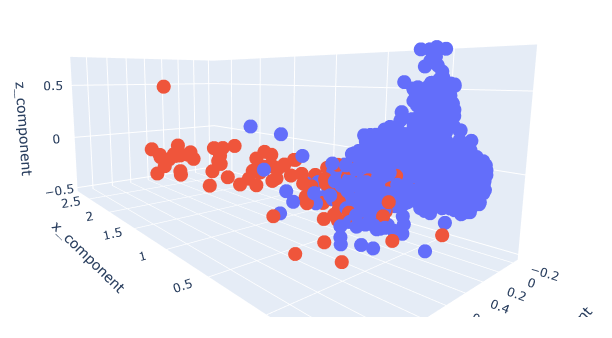
\includegraphics[width=9cm, scale=1]{images/scatter_cluster_good}
    \captionsetup{type=figure}
	\captionof{figure}{Scatter Plot Machine-2-3}
         \label{scatter-cluster-good}
\end{center}
\begin{center}
	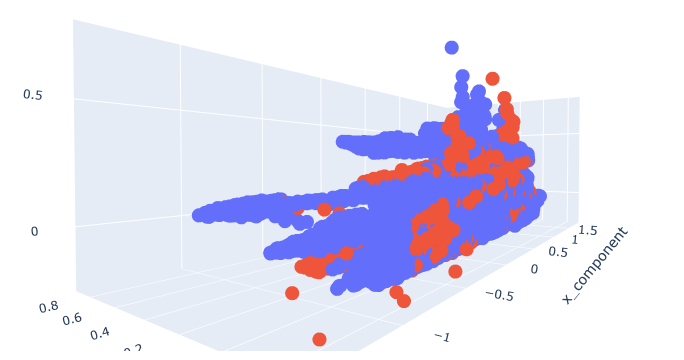
\includegraphics[width=9cm, scale=1]{images/scatter_cluster}
    \captionsetup{type=figure}
	\captionof{figure}{Scatter Plot Machine-1-7}
      \label{scatter-cluster-bad}
\end{center}

\newpage
\subsubsection{Rank aggregation}
A questo punto ci si può concentrare sulle varie tecniche di aggregazione. L'aggregazione è stata fatta andando a considerare sempre tutte e tre le metriche surrogate, senza fare eccezione nonostante ci fossero dataset in cui alcune metriche surrogate avevano performance particolarmente basse. 
Si può vedere, in Tabella \ref{agg-results}, come il metodo ottimale di aggregazione, che ricordiamo essere NP-Hard, produca i risultati migliori. 
I valori medi rispetto ai dataset si aggirano intorno al range [0.4,0.6], in linea con le performance di Model Centrality e migliori rispetto a Performance on Injected Synthetic Anomalies e Clustering Cohesion. Questo vuol dire che i metodi di aggregazione riescono comunque a produrre buoni risultati nonostante le metriche surrogate non funzioni sempre bene. 
Questo tipo di aggregazione permette di avere risultati migliori quando non si ha la certezza che una sola metrica surrogata sia sufficiente. Potrebbe comunque essere utile un'analisi specifica per andare a prendere in considerazione soltanto quelle metriche surrogate, o più nello specifico i metodi utilizzati al loro interno (Round Robin, Majority Vote, Sampling per Model Centrality o Scale, Spike, Growing, Mix per Performance on Injected Synthetic Anomalies), che potrebbero funzionare meglio per uno specifico dataset. 
Considerando le metriche surrogate singolarmente, quella più performante è Model Centrality. La motivazione di ciò può risiedere nel fatto che utilizzando le informazioni provenienti da tutti i modelli si riescono a ottenere risultati migliori a quelle metriche che trattano gli output dei modelli in maniera indipendente.

Il metodo di AVG Score è il più semplice ma produce anche risultati più scarsi. Nel nostro caso, con sole 3 metriche surrogate che vengono aggregate, l'utilizzo del metodo ottimale risulta la scelta migliore nonostante la complessità temporale sia più alta. Se si fossero prese in considerazione più metriche, questo approccio non sarebbe più possibile proprio per la natura NP-Hard del problema.

\begin{table}[]
	\caption{\label{agg-results}Risultati di correlazione per aggregazione}
	\resizebox{\linewidth}{!}{%
		\begin{tabular}{|l||l|l|l|l||l|l|l|l||l|l|l|l|} 
			\hline
			Dataset           & \multicolumn{4}{c||}{SCORE CORRELATION} & \multicolumn{8}{c|}{RANK CORRELATION}                            \\ 
			\hline
			\multirow{2}{*}{} & \multicolumn{4}{c||}{PEARSON}           & \multicolumn{4}{c||}{KENDALL}  & \multicolumn{4}{c|}{SPEARMAN}   \\ 
			\cline{2-13}
			                & score & borda & rborda & opt   & score & borda & rborda & opt   & score & borda        & rborda & opt   \\ 
			\hline
			2\_annthyroid   & 0.795 & 0.644 & 0.394  & 0.768 & 0.486 & 0.499 & 0.382  & 0.586 & 0.550 & 0.587        & 0.331 & 0.696 \\ 
			\hline
			6\_cardio       & 0.758 & 0.589 & 0.409  & 0.597 & 0.578 & 0.416 & 0.374  & 0.550 & 0.693 & 0.545        & 0.447 & 0.572 \\ 
			\hline
			11\_donors      & 0.404 & 0.633 & 0.164  & 0.541 & 0.348 & 0.553 & 0.129  & 0.573 & 0.430 & 0.672        & 0.195 & 0.683 \\ 
			\hline
			20\_letter      & 0.595 & 0.561 & 0.436  & 0.664 & 0.493 & 0.423 & 0.418  & 0.546 & 0.606 & 0.557        & 0.406 & 0.639 \\ 
			\hline
			23\_mammography & 0.681 & 0.770 & 0.489  & 0.793 & 0.495 & 0.587 & 0.427  & 0.654 & 0.599 & 0.748        & 0.427 & 0.822 \\ 
			\hline
			27\_PageBlocks  & 0.843 & 0.753 & 0.395  & 0.860 & 0.594 & 0.551 & 0.323  & 0.659 & 0.690 & 0.713        & 0.375 & 0.822 \\ 
			\hline
			31\_satimage-2  & 0.574 & 0.761 & 0.489  & 0.730 & 0.428 & 0.559 & 0.389  & 0.630 & 0.584 & 0.736        & 0.457 & 0.816 \\ 
			\hline
			32\_shuttle     & 0.562 & 0.843 & 0.696  & 0.899 & 0.500 & 0.644 & 0.592  & 0.755 & 0.590 & 0.806        & 0.674 & 0.882 \\ 
			\hline
			38\_thyroid     & 0.623 & 0.616 & 0.367  & 0.644 & 0.477 & 0.451 & 0.390  & 0.526 & 0.536 & 0.561        & 0.334 & 0.655 \\ 
			\hline
			40\_vowels      & 0.765 & 0.813 & 0.578  & 0.807 & 0.649 & 0.632 & 0.430  & 0.661 & 0.833 & 0.816        & 0.546 & 0.858 \\ 
			\hline
			41\_Waveform    & 0.581 & 0.623 & 0.536  & 0.521 & 0.560 & 0.464 & 0.435  & 0.576 & 0.673 & 0.586        & 0.540 & 0.668 \\ 
			\hline
			machine-1-1     & 0.464 & 0.556 & 0.311  & 0.620 & 0.486 & 0.434 & 0.292  & 0.564 & 0.526 & 0.581        & 0.302 & 0.684 \\ 
			\hline
			machine-1-2     & 0.820 & 0.797 & 0.423  & 0.777 & 0.623 & 0.591 & 0.423  & 0.632 & 0.841 & 0.753        & 0.413 & 0.782 \\ 
			\hline
			machine-1-3     & 0.245 & 0.686 & 0.416  & 0.623 & 0.294 & 0.596 & 0.437  & 0.561 & 0.291 & 0.689        & 0.413 & 0.651 \\ 
			\hline
			machine-1-4     & 0.411 & 0.577 & 0.390  & 0.475 & 0.390 & 0.491 & 0.397  & 0.496 & 0.470 & 0.589        & 0.449 & 0.512 \\ 
			\hline
			machine-1-5     & 0.496 & 0.581 & 0.423  & 0.477 & 0.429 & 0.411 & 0.480  & 0.460 & 0.567 & 0.537        & 0.448 & 0.589 \\ 
			\hline
			machine-1-6     & 0.476 & 0.302 & 0.259  & 0.554 & 0.376 & 0.342 & 0.292  & 0.361 & 0.363 & 0.381        & 0.291 & 0.437 \\ 
			\hline
			machine-1-7     & 0.413 & 0.354 & 0.250  & 0.375 & 0.372 & 0.314 & 0.312  & 0.378 & 0.500 & 0.410        & 0.322 & 0.451 \\ 
			\hline
			machine-1-8     & 0.385 & 0.417 & 0.243  & 0.507 & 0.319 & 0.347 & 0.254  & 0.406 & 0.392 & 0.311        & 0.227 & 0.511 \\ 
			\hline
			machine-2-1     & 0.606 & 0.510 & 0.396  & 0.559 & 0.427 & 0.436 & 0.395  & 0.497 & 0.554 & 0.446        & 0.350 & 0.513 \\ 
			\hline
			machine-2-2     & 0.761 & 0.658 & 0.426  & 0.623 & 0.434 & 0.492 & 0.434  & 0.478 & 0.560 & 0.577        & 0.418 & 0.607 \\ 
			\hline
			machine-2-3     & 0.861 & 0.876 & 0.825  & 0.895 & 0.709 & 0.783 & 0.632  & 0.760 & 0.816 & 0.881        & 0.805 & 0.886 \\ 
			\hline
			machine-2-4     & 0.453 & 0.497 & 0.432  & 0.511 & 0.451 & 0.431 & 0.489  & 0.496 & 0.541 & 0.513        & 0.473 & 0.572 \\ 
			\hline
			machine-2-5     & 0.129 & 0.425 & 0.320  & 0.297 & 0.241 & 0.396 & 0.363  & 0.399 & 0.294 & 0.346        & 0.378 & 0.469 \\ 
			\hline
			machine-2-6     & 0.725 & 0.726 & 0.312  & 0.789 & 0.498 & 0.531 & 0.314  & 0.584 & 0.634 & 0.676        & 0.335 & 0.738 \\ 
			\hline
			machine-2-7     & 0.792 & 0.776 & 0.554  & 0.839 & 0.591 & 0.576 & 0.457  & 0.626 & 0.730 & 0.717        & 0.600 & 0.762 \\ 
			\hline
			machine-2-8     & 0.933 & 0.839 & 0.575  & 0.903 & 0.774 & 0.726 & 0.505  & 0.763 & 0.870 & 0.825        & 0.566 & 0.882 \\ 
			\hline
			machine-2-9     & 0.587 & 0.624 & 0.532  & 0.629 & 0.535 & 0.444 & 0.484  & 0.549 & 0.623 & 0.584        & 0.480 & 0.580 \\ 
			\hline
			machine-3-1     & 0.554 & 0.624 & 0.451  & 0.670 & 0.482 & 0.486 & 0.398  & 0.578 & 0.565 & 0.574        & 0.454 & 0.661 \\ 
			\hline
			machine-3-2     & 0.661 & 0.687 & 0.497  & 0.683 & 0.608 & 0.573 & 0.478  & 0.607 & 0.779 & 0.656        & 0.566 & 0.676 \\ 
			\hline
			machine-3-3     & 0.065 & 0.287 & 0.256  & 0.341 & 0.112 & 0.242 & 0.325  & 0.356 & 0.154 & 0.261        & 0.329 & 0.415 \\ 
			\hline
			machine-3-4     & 0.239 & 0.387 & 0.394  & 0.203 & 0.392 & 0.332 & 0.325  & 0.428 & 0.351 & 0.373        & 0.374 & 0.395 \\ 
			\hline
			machine-3-5     & 0.844 & 0.622 & 0.454  & 0.675 & 0.744 & 0.503 & 0.463  & 0.569 & 0.866 & 0.582        & 0.437 & 0.648 \\ 
			\hline
			machine-3-6     & 0.363 & 0.390 & 0.294  & 0.401 & 0.318 & 0.385 & 0.270  & 0.437 & 0.305 & 0.300        & 0.260 & 0.523 \\ 
			\hline
			machine-3-7     & 0.355 & 0.496 & 0.497  & 0.424 & 0.425 & 0.418 & 0.436  & 0.520 & 0.485 & 0.419        & 0.404 & 0.536 \\ 
			\hline
			machine-3-8     & 0.586 & 0.660 & 0.534  & 0.630 & 0.468 & 0.500 & 0.427  & 0.552 & 0.589 & 0.597        & 0.535 & 0.642 \\ 
			\hline
			machine-3-9     & 0.496 & 0.677 & 0.526  & 0.590 & 0.496 & 0.529 & 0.448  & 0.604 & 0.555 & 0.622        & 0.526 & 0.701 \\ 
			\hline
			machine-3-10    & 0.021 & 0.365 & 0.382  & 0.262 & 0.152 & 0.259 & 0.379  & 0.313 & 0.175 & 0.327        & 0.343 & 0.395 \\ 
			\hline
			machine-3-11    & 0.590 & 0.612 & 0.553  & 0.639 & 0.467 & 0.449 & 0.426  & 0.511 & 0.469 & 0.596        & 0.558 & 0.642 \\ 
			\hline
			AVG             & 0.552 & 0.605 & 0.433  & 0.610 & 0.467 & 0.482 & 0.401  & 0.544 & 0.555 & 0.576        & 0.430 & 0.640 \\ 
			\hline
			STD             & 0.22  & 0.154 & 0.127  & 0.177 & 0.141 & 0.115 & 0.09   & 0.107 & 0.177 & 0.156        & 0.121 & 0.138 \\
			\hline
		\end{tabular}
	}
\end{table}

\newpage
\subsubsection{Variazione di $k$}
Interessante vedere come Robust Borda, che sulla carta dovrebbe avere performance migliori, sia in verità inferiore alla sua versione standard Borda. Un motivo di ciò può risiedere nel fatto che ci sono modelli che sono nelle posizioni più alte per quanto riguarda alcune metriche surrogate ma che performano sufficientemente male in altre e vengono quindi penalizzate troppo.
Si può vedere infatti, nella Figura \ref{varying-k}, che all'aumentare del fattore $k$ aumentano le performance di Robust Borda, fino arrivare al valore massimo con $k=N$, ovvero Borda.


\begin{figure}[t]
	\centering
	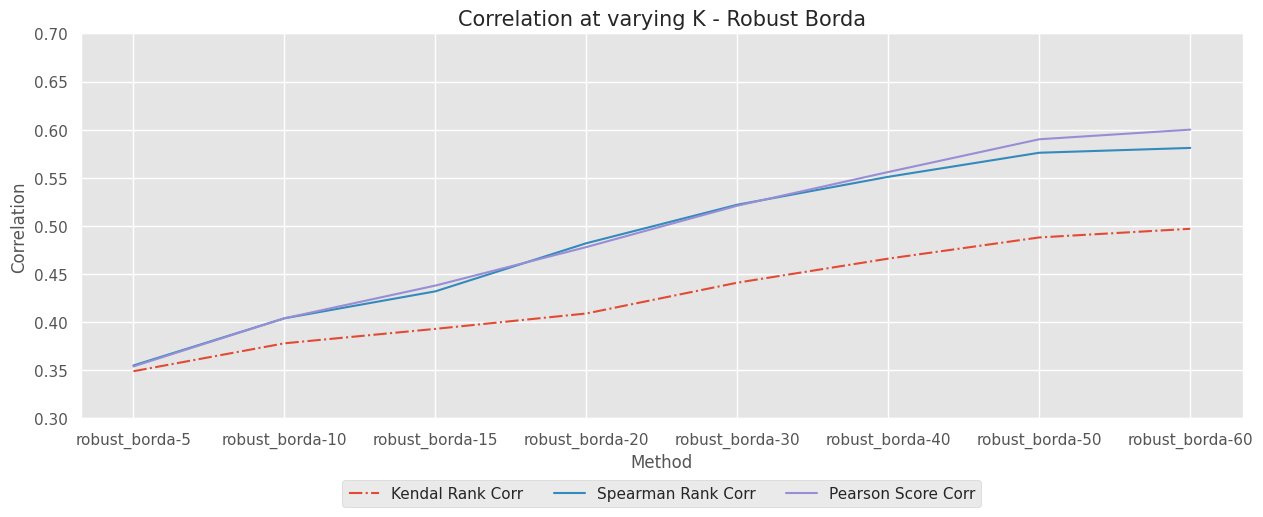
\includegraphics[width=14cm, scale=1]{images/varying-k}
	\caption{Performance di Robust Borda al variare del parametro $k$}
	\label{varying-k}
		
\end{figure}

\subsubsection{Ripetitività}
Alcune metriche surrogate includono al loro interno un fattore di casualità, in particolare Sampling e tutte e 4 le tecniche di Anomaly Injection. Il primo metodo può variare ad ogni suo utilizzo in quanto per ogni sample viene scelto casualmente quale modello usare come riferimento per l'etichetta. Invece i metodi di Anomaly Injection genereranno sempre anomalie differenti in quanto sia la posizione che il magnitudo di anomalia cambia ogni volta.
Per questo motivo è stata fatta anche un'analisi andando a ripetere il Model Selection su due dataset per 5 volte.
Nella Figura \ref{score-box} è possibile vedere un Box Whisker Plot sugli score prodotti da Model Selection per ognuna delle metriche e metodi. Alcuni di questi non includono casualità come Round Robin, Majority Vote, Score Correlation e Score Clustering, di conseguenza il valore è uguale ad ogni iterazione. Al contrario gli altri vedono differire il valore ad ogni iterazione, chi più chi meno. In generale, vi è un range che varia di circa 0.05 punti.

\begin{figure}[t]
	\centering
	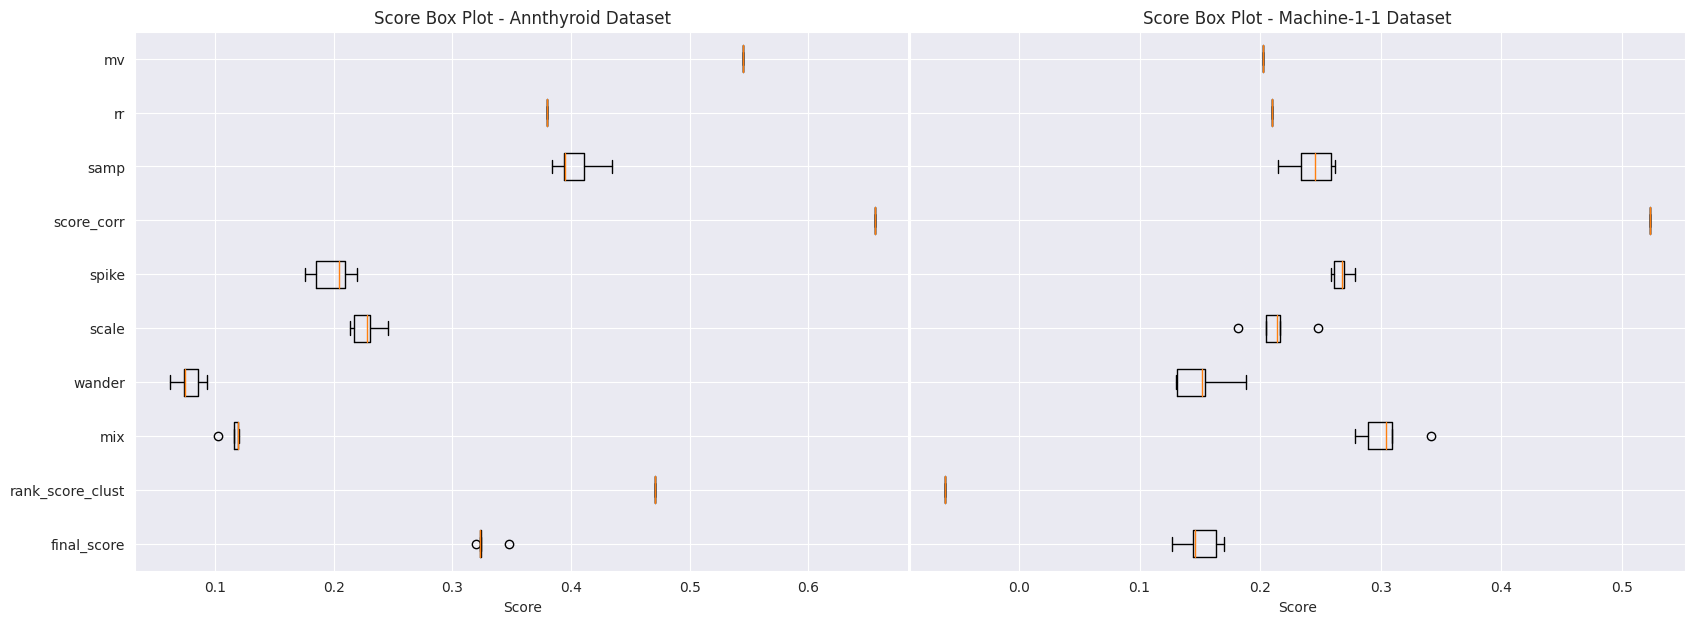
\includegraphics[width=16cm, scale=1]{images/score_box}
	\caption{Score Box Plot su Annthyroid (sinistra) e Machine-1-1 (destra)}
	\label{score-box}
	
\end{figure}

Queste differenze negli score vanno anche ad impattare poi il coefficiente di correlazione Kendall rispetto al Ranking Supervisionato. Anche qui, come prima, le differenze sono esigue ma sempre presenti; Figura \ref{kendall-box}.

\begin{figure}[t]
	\centering
	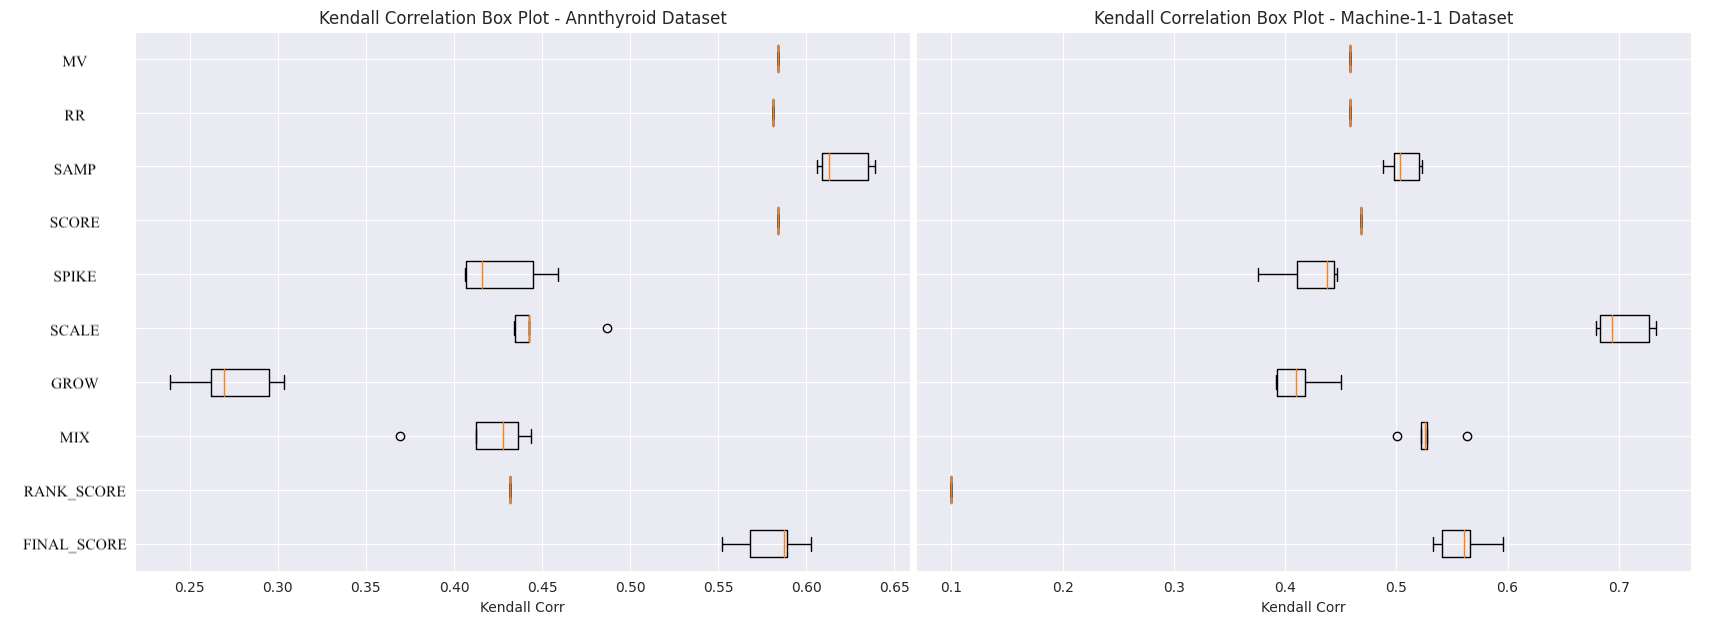
\includegraphics[width=16cm, scale=1]{images/kendall_box}
	\caption{Kendall Correlation Box Plot su Annthyroid (sinistra) e Machine-1-1 (destra)}
	\label{kendall-box}
		
\end{figure}


\subsubsection{Intersezione dei quantili}
Oltre a valutare le performance sullo score di correlazione tra il ranking non supervisionato e quello supervisionato, può risultare utile cambiare punto di vista e comparare i ranking dal punto di vista dell'intersezione dei quantili.
Per questa valutazione sono stati ordinati i ranking per il loro score e poi sono stati divisi in 2 o 4 quantili. Successivamente viene calcolata l'intersezione del quantile di un ranking con il corrispondente dell'altro ranking.
Come mostrato nella Figura \ref{quantile-intersection}, si può notare come dividendo in 4 quantili, l'intersezione produca uno score di circa 0.55 per i primi 3 quantili, segno che faccia più fatica nel classificare correttamente le performance dei modelli nelle posizioni più alte. Il quarto quantile però ha un punteggio di circa 0.77, segno che l'algoritmo di Model Selection sa distinguere i modelli più performanti con quelli meno performanti.

Possiamo quindi concludere che mentre il model Selection non supervisionato non sia molto preciso nel trovare il modello migliore tra quelli con performance buone, è comunque in grado di riconoscere abbastanza bene quelli peggiori. A confermare questa ipotesi il calcolo dell'intersezione dei quantili con soltanto due quantili, producendo uno score di intersezione di circa \(0.8\).

\begin{figure}[t]
	\centering
	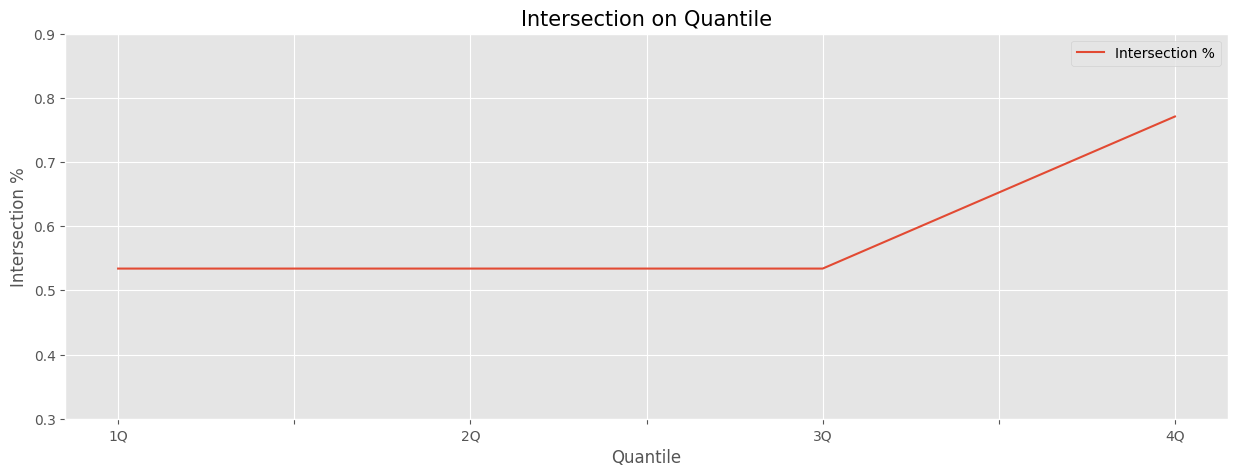
\includegraphics[width=14cm, scale=1]{images/4quantile}
	\caption{Intersezione tra quantili}
	\label{quantile-intersection}
		
\end{figure}

\subsubsection{Confronto con baseline}
In questa sezione vengono proposte, rispetto a tutti i dataset, le performance del miglior modello secondo Model Selection confrontate a tre baseline:
\begin{enumerate}
\item Random: viene preso casualmente, per ogni dataset, un modello dalla lista dei modelli candidati
\item AVG: ovvero il modello con le performance medie migliori rispetto a tutti i dataset. Valutato usando le etichette con la metrica F1 Score
\item Best: per ogni dataset viene preso il miglior modello secondo F1 Score
\end{enumerate}
In Tabella \ref{wins} sono riportati i conteggi delle vittorie (o pareggi) rispetto a tutti e 39 i dataset di benchmark del miglior modello secondo Model Selection contro le tre baseline. I risultati proposti fanno riferimento sia alle tre metriche surrogate prese singolarmente, considerando anche le varie misure interne di ognuna, sia al punteggio finale prodotto dall'aggregazione delle tre metriche surrogate utilizzando Round Robin, Mix e Clustering Cohesion con il metodo ottimale di Kemeny-Young.
I risultati vanno a confermare quanto già detto nelle sezioni precedenti. La metrica di Model Centrality ha un numero di vittorie maggiore rispetto alle altre due, e nello specifico Round Robin e Sampling hanno il numero di vittorie più alto in assoluto.
I vari metodi di Anomaly Injection hanno un numero di vittorie comparabile, in linea anche con la metrica di Clustering Cohesion. Final Score rappresenta le vittorie utilizzando il ranking aggregato con Kemeny-Young e risulta meno performante se paragonato esclusivamente a Model Centrality.
Confrontando invece il numero di vittorie del ranking aggregato rispetto alle baseline, l'algoritmo di Model Selection trova dei modelli che riescono a vincere 29 volte rispetto ad una selezione casuale. Questo significa che su 39 dataset, 29 volte Model Selection è risultato più utile rispetto ad una selezione casuale. Contro il modello che ha le performance medie migliori, in questo caso KNN, Model Selection ha vinto 23 volte. Non un risultato incoraggiante, considerando che vengono allenati molti modelli per poi ottenere delle performance comparabili ad un unico modello (KNN). La situazione migliorerebbe se si andasse a considerare soltanto Model Centrality: rispettivamente 36 e 30 vittorie su 39. Questo è un risultato incoraggiante, segno che metriche non supervisionate possono, se sviluppate correttamente, essere sufficientemente buone.
Infine il numero di pareggi, ovvero quante volte Model Centrality riesce a trovare effettivamente il modello migliore, sono molto bassi, segno che le metriche surrogate implementate non sono sufficienti.

\begin{table}[]
\centering
\resizebox{\textwidth}{!}{%
\begin{tabular}{|cl|l|l|l|l|l|l|l|l|l|l|}
\hline
\multicolumn{2}{|l|}{}                                             & rr & mv & score\_corr & samp & scale & spike & wander & mix & rank\_score\_clust & final\_score \\ \hline
\multicolumn{1}{|c|}{\multirow{3}{*}{vittorie o pareggi}} & random & 36 & 34 & 32          & 36   & 29    & 27    & 28     & 26  & 29                 & 29           \\ \cline{2-12} 
\multicolumn{1}{|c|}{}                                    & avg    & 30 & 26 & 27          & 30   & 20    & 18    & 18     & 19  & 18                 & 23           \\ \cline{2-12} 
\multicolumn{1}{|c|}{}                                    & best   & 3  & 2  & 2           & 2    & 4     & 4     & 3      & 3   & 2                  & 3            \\ \hline
\end{tabular}%
}
\captionof{table}{Numero di vittorie o pareggi del miglior modello secondo Model Selection rispetto alle baseline. Conteggio rispetto a tutti i dataset (39).}\label{wins}
\end{table}

\newpage
\section{Risultati SKF}
Il progetto di tesi è nato da una collaborazione tra ALTEN e SKF quindi una parte dedicata a quest'ultima è necessaria. Come introdotto nel Capitolo \ref{chap:skf} però, i dati prodotti dai sensori installati sui macchinari della catena di montaggio non sono sufficientemente completi per riuscire a fornire una valutazione completa dell'algoritmo di Model Selection. La mancanza di etichette e di uno storico delle manutenzioni effettuate in aggiunta al fatto che non tutte le macchine sono mappate dai sensori, rende complicato valutare i modelli di Anomaly Detection. La presenza dei dati MVM aiuta poco alla causa per tre motivi: (1) non tutte le macchine hanno sensori installati, (2) la frequenza con la quale vengono registrati i dati CoMo e troppo bassa e (3) la correlazione tra i valori dei sensori e la qualità finale non è certo da dare per scontata. Potrebbero esserci fattori aggiuntivi come la qualità del materiale utilizzato per la produzione oppure anche problemi ai macchinari che non vengono captati dai sensori. 
Nonostante ciò, viene svolta una valutazione usando MVM come riferimento. Prima viene eseguito l'algoritmo di Model Selection non supervisionato sul dataset di uno specifico macchinario andando a produrre una serie di ranking e ottenendo così il modello in prima posizione, successivamente viene usato questo per andare a fare la prediction sui dati sempre dello stesso macchinario. Infine si utilizzano i dati di MVM per:
\begin{itemize}
        \item Calcolare la qualità media per ogni intervallo di 10 minuti ed utilizzare il valore come label: se supera la soglia di qualità Q1 per la banda A avrà label 1, altrimenti 0. Queste nuove etichette sono usate per essere confrontate con la predizione del miglior modello secondo Model Selection.
	\item Calcolare il numero di volte in cui un cuscinetto a sfera supera la soglia della banda A per la classe Q1 nell'intervallo di 10 minuti e paragonare questi numeri tra i punti segnalati come anomali dal modello con i punti segnalati come normali.
	
\end{itemize}
L'assunzione forte che è stata fatta è che situazione anomale di un macchinario portino a qualità del prodotto finito più bassa, ovvero a valori di MVM più alti. Quello che si spera di ottenere è vedere questa assunzione all'atto pratico, ovvero con valori di MVM mediamente più alti (qualità più bassa) per quei punti considerati anomali da un modello rispetto ai punti considerati normali.
Per completezza vengono anche proposti i risultati del modello peggiore secondo Model Selection, in modo da compararlo con il migliore.

\subsection{Dataset}
I dataset di SKF sono stati introdotti e dettagliati nel Capitolo \ref{chap:skf}. Per questa fase di valutazione vengono usati sia i dati di MVM, più nello specifico viene usata la banda A riguardante gli errori geometrici provenienti dalla fase di rettifica. Questo perché si è deciso di concentrarsi esclusivamente sul macchinario che, per motivi di riservatezza, chiameremo M1. Questo macchinario è il primo nella linea di produzione ed effettua la rettifica, quindi direttamente interessato alla banda A.
Per la fase di training è stato scelto il periodo che va da gennaio a aprile 2022 in quanto i dati in quel periodo risultavano i più puliti ed i più stabili da un punto di vista di oscillazioni o data-change. Mentre per la fase di prediction viene usato come riferimento il periodo maggio-giugno 2022.



\subsection{Thresholding}
Prima di procedere al training del modello è necessario avere un riferimento sulla percentuale di anomalie nel dataset. A questo scopo è stato utilizzato il metodo ${\gamma}GMM$ introdotto nel Capitolo \ref{chap:methods}.
Questo algoritmo riceve in input la stessa lista di modelli candidati usati poi nel Model Selection. Dopo che i modelli sono stati allenati sul dataset di training (senza andare ad indicare il fattore di contaminazione) sono stati usati gli output score prodotti da ognuno di questi per computare la distribuzione di probabilità multivariata delle anomalie.
Il risultato prodotto da questa tecnica di thresholding è 0.05, ovvero il 5\% di punti vengono considerati anomali. Un dato ragionevole confermato dagli esperti.


\subsection{Risultati}
L'algoritmo di Model Selection, eseguito sul dataset del macchinario M1 utilizzando come modelli la medesima lista utilizzata con i dataset di benchmark, ha prodotto i seguenti risultati:


\begin{table}[H]
	\begin{minipage}{.5\textwidth}
		\centering
		\resizebox{\columnwidth}{!}{%
			\begin{tabular}{|l|l|l|l|l|l|} 
				\hline
				\textbf{\#} & \textbf{Model} & \textbf{RR} & \textbf{MIX} & \textbf{CC} & \textbf{Final} \\ 
				\hline
				1           & KDE            & 0.544       & 0.391        & 0.549       & 0.990            \\ 
				\hline
				2           & CBLOF\_4       & 0.539       & 0.388        & 0.501       & 0.988            \\ 
				\hline
				3           & MCD            & 0.508       & 0.483        & 0.530       & 0.955            \\ 
				\hline
				4           & IForest\_200   & 0.509       & 0.320        & 0.554       & 0.938            \\ 
				\hline
				5           & OCSVM\_poly    & 0.452       & 0.386        & 0.542       & 0.920            \\ 
				\hline
				6           & OCSVM\_sig     & 0.452       & 0.384        & 0.542       & 0.919            \\ 
				\hline
				7           & PCAODetector   & 0.552       & 1.000        & 0.510       & 0.901            \\ 
				\hline
				8           & KPCA           & 0.548       & 0.335        & 0.528       & 0.899            \\ 
				\hline
				9           & PCA            & 0.552       & 0.077        & 0.510       & 0.893            \\ 
				\hline
				10          & KNN\_10        & 0.562       & 0.286        & 0.474       & 0.830            \\
				\hline
			\end{tabular}
			}\captionof{table}{Top 10}
	\end{minipage}
	\begin{minipage}{.5\textwidth}
		\centering
		\resizebox{\columnwidth}{!}{%
			\begin{tabular}{|l|l|l|l|l|l|} 
				\hline
				\textbf{\#} & \textbf{Model} & \textbf{RR} & \textbf{MIX} & \textbf{CC} & \textbf{Final} \\ 
				\hline
				70          & Telemanom       & 0.005       & 0.029        & 0.314       & 0.030            \\ 
				\hline
				69          & SO\_GAAL      & 0.090       & 0.997        & 0.237       & 0.030            \\ 
				\hline
				68          & DeepSVDD       & 0.214       & 0.120        & 0.348       & 0.035            \\ 
				\hline
				67          & ALAD           & 0.071       & 0.092        & 0.375       & 0.067            \\ 
				\hline
				66          & SOS            & 0.218       & 0.143        & 0.391       & 0.098            \\ 
				\hline
				65          & SOS\_7         & 0.228       & 0.143        & 0.370       & 0.118            \\ 
				\hline
				64          & FeatureBagging & 0.335       & 0.024        & 0.406       & 0.127            \\ 
				\hline
				63          & LOF            & 0.337       & 0.065        & 0.390       & 0.136            \\ 
				\hline
				62          & PCAODetector   & 0.103       & 0.997        & 0.394       & 0.136            \\ 
				\hline
				61          & ABOD           & 0.423       & 0.054        & 0.391       & 0.139            \\
				\hline
			\end{tabular}}\captionof{table}{Worst 10}
	\end{minipage}
\end{table}




Sono proposti i primi 10 e gli ultimi 10 modelli con i relativi score finali. Le metriche surrogate utilizzate sono state (1) Round Robin per Model Centrality, (2) Mix per Performance on Injected Synthetic Anomalies e (3) Clustering Cohesion. La tecnica di aggregazione utilizzata è stato il metodo ottimale di Kemeny-Young.
Il primo modello è KDE, ovvero Kernel Density Estimation, ed in generale i metodi di Machine Learning hanno uno score più alto di quelli Deep Learning. Situazione rimarcata dal fatto che per le ultime 10 posizioni sono presenti 4 metodi di Deep Learning. Una spiegazione a questo fenomeno risiede nel fatto che questi ultimi modelli hanno score di Model Centrality e Anomaly Injection molto bassi. Eccezione per SO-GALL che riesce a riconoscere quasi perfettamente tutte le anomalie sintetiche iniettate. Gli Score di Clustering Cohesion vanno anche questa volta a favorire metodi di Machine Learning, anche se in misura più lieve. Infatti i modelli come DeepSVDD o ALAD riescono a  raggiungere punteggi intorno al 0.35.
Model Centrality va sicuramente a favorire quei modelli che producono output simile tra di loro, implicando una forte varianza dei risultati sulla base di quali modelli candidati vengono passati all'algoritmo di Model Selection. Potrebbe essere il caso che i modelli di Deep Learning siano effettivamente i migliori, ma essendo pochi rispetto al numero totale di modelli considerati, il loro punteggio di Model Centrality va abbassandosi. In questi casi, per trovare conferma, un'analisi visiva delle anomalie rilevate può risultare utile.

\subsubsection{Anomalie rilevate}
Attraverso un grafico a linee con barre verticali per rappresentare i punti temporali rilevati come anomalia, possiamo notare nella Figura \ref{kde} come KDE, ovvero il miglior modello, riesca a riconoscere bene i punti di Spike o gli intervalli di Scale in cui certi sensori raggiungono valori sufficientemente distanti da un comportamento standard. Il modello peggiore, ovvero Telemanom (Figura \ref{worst_clf}), raggruppa tutti i punti anomali in un unico intervallo continuo nonostante ci siano dei punti temporali che non presentino, ad occhio, un comportamento anomalo.

\begin{figure}[t]
	\centering
	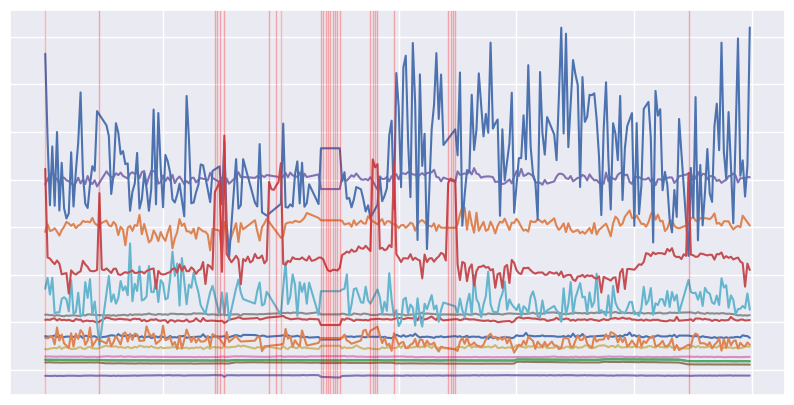
\includegraphics[width=14cm, scale=1]{images/kde}
	\caption{Anomalie Rilevate da KDE}
	\label{kde}
	
\end{figure}

\begin{figure}[t]
	\centering
	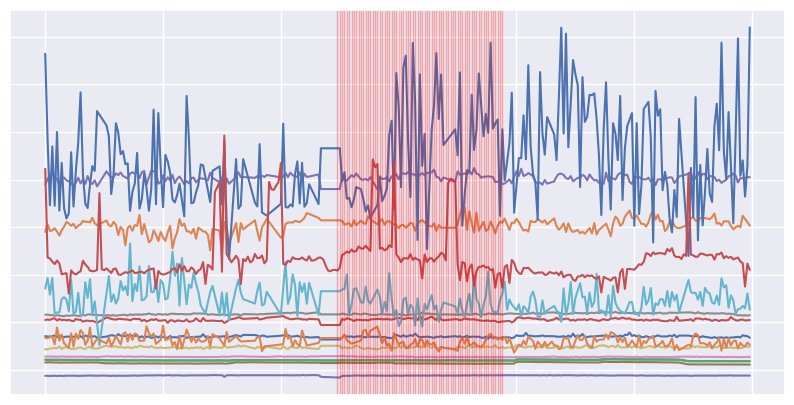
\includegraphics[width=14cm, scale=1]{images/worst_clf}
	\caption{Anomalie Rilevate da Telemanom}
	\label{worst_clf}
	
\end{figure}

Passando ad un plot scatter dopo aver ridotto la dimensionalità dei punti a 2 dimensioni tramite PCA, possiamo notare in Figura \ref{kde_scatter} due cluster principali con punti sparsi nel mezzo. I punti anomali trovati da KDE si trovano principalmente nel cluster più piccolo a destra e nei punti sparsi nel piano. Mentre il cluster blu a sinistra risulta ben omogeneo.
Telemanom invece etichetta come anomali principalmente i punti all'interno del cluster di sinistra, risultando in una separazione meno chiara, Figura \ref{worst_clf_scatter}.
Ovviamente non si ha la certezza che il cluster di destra sia effettivamente composto da tutti punti anomali, ma chiaramente un comportamento fuori dal normale c'è in quanto la grande maggioranza dei dati, risiedenti nel cluster di sinistra, possiedono valori molto diversi.


\begin{figure}[t]
	\centering
	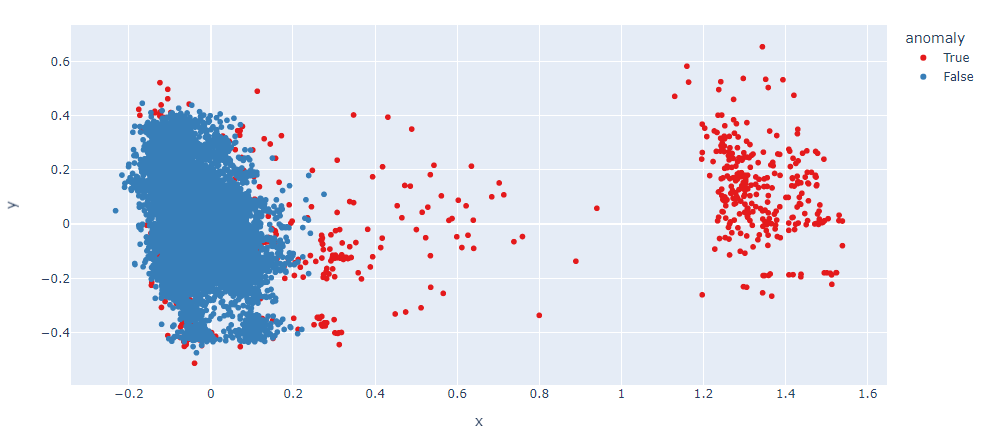
\includegraphics[width=14cm, scale=1]{images/kde_scatter}
	\caption{Scatter Plot delle anomalie KDE}
	\label{kde_scatter}
		
\end{figure}




\begin{figure}[t]
	\centering
	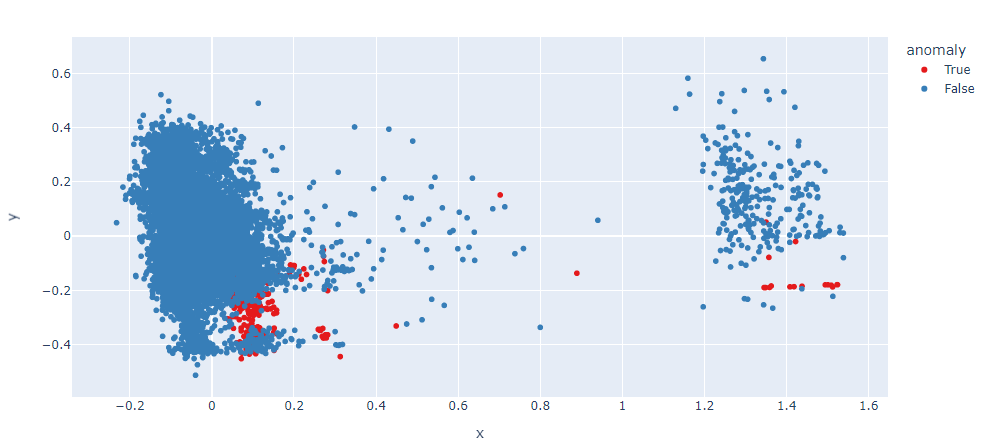
\includegraphics[width=14cm, scale=1]{images/worst_clf_scatter}
	\caption{Scatter Plot delle anomalie Telemanom}
	\label{worst_clf_scatter}
		
\end{figure}

\subsubsection{Confronto qualità}
In questa sezione viene fatto un confronto tra le anomalie rilevate e la qualità. Come anticipato più volte, la qualità non è da considerarsi un perfetto indicatore delle anomalie: 
\begin{itemize}
	\item La qualità viene registrata ogni due secondi mentre i dati CoMo ogni 10 minuti. Di conseguenza la qualità viene aggregata con una media, andando a nascondere, nel calcolo aggregato, i valori più alti che sono anche i più rari. Usare altre tecniche di aggregazione come Min o Max non è immediato in quanto avrebbe poi favorito troppo o troppo poco la presenza di valori di qualità estremi.
	\item Analizzando un solo macchinario non è possibile avere una situazione completa della linea di produzione: una qualità bassa può essere data da un'anomalia su un macchinario non mappato. Ma anche analizzando tutti i macchinari insieme non è certo che la qualità sia correlata al 100\% con i dati CoMo. Ci possono essere fattori come la qualità del materiale o degli oli, o altri movimenti dei macchinari non registrati che impattano la qualità. Producendo quindi valori di qualità bassa nonostante registrazioni CoMo nella norma. Oppure il contrario, ovvero registrazioni CoMo anomale ma che non impattano la qualità.
\end{itemize}

Prima di proseguire è necessario applicare una trasformazione ai dati. Il macchinario analizzato M1 è il primo della linea di montaggio, mentre il macchinario di misura qualità MVM è posto alla fine. Il cuscinetto a sfera dal momento che parte impiega un tempo ${\nabla}t$ ad arrivare ad MVM e quindi essere registrato per la misura di qualità. Per allineare quindi la registrazione CoMo di M1 con la registrazione di MVM è necessario traslare di ${\nabla}t$ l'indice temporale della tabella MVM.

Nelle prossime due immagini possiamo vedere lo stesso scatter plot di prima, ma andando a colorare i punti sulla base della correlazione tra punti rilevati come anomali da KDE e Telemanom, e i punti registrati come bassa qualità. Per bassa qualità si intende quando la media delle qualità per ogni intervallo di 10 minuti supera la soglia Q1 per la banda A. Le correlazioni sono così spiegate:
\begin{itemize}
	\item \textit{true positive} indica che il punto è rilevato sia come anomalo che di bassa qualità
	\item \textit{true negative} indica che il punto è rilevato sia come non anomalo che di qualità normale
	\item \textit{false negative} indica che il punto è rilevato come non anomalo ma la qualità è bassa
	\item \textit{false positive} indica che il punto è rilevato come anomalo ma la qualità è normale
\end{itemize}

La Figura \ref{kde_quality} rappresenta lo scatter con KDE, la maggior parte dei punti del cluster di sinistra viene correttamente identificato come true-negative ma sono presenti un numero non indifferente di falsi negativi. Il cluster di destra, così come i punti sparsi nel mezzo, vengono identificati per circa metà come falsi positivi e metà come true positive.
\begin{figure}[t]
	\centering
	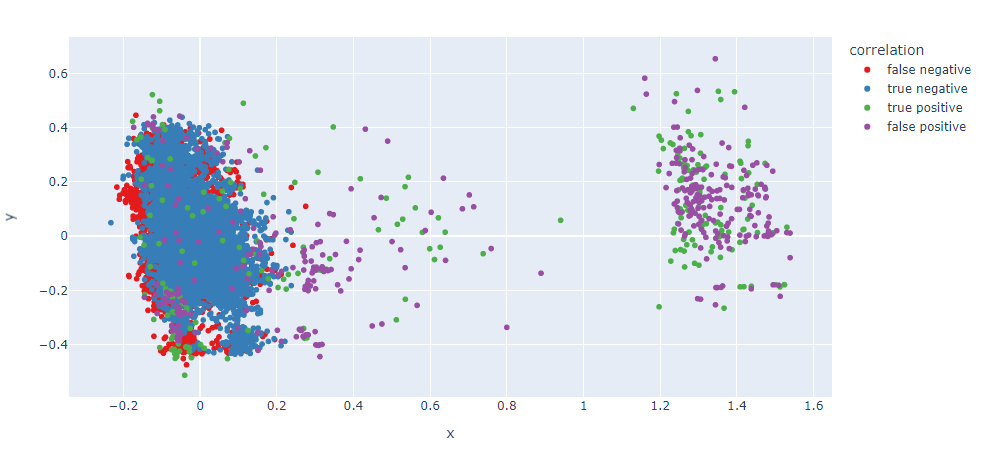
\includegraphics[width=14cm, scale=1]{images/correlation_ssb1_quality_plot.png}
	\caption{Scatter Plot Correlazione Qualità KDE}
	\label{kde_quality}
\end{figure}

Con Telemanom, Figura \ref{worst_clf_quality} la situazione non è migliore, in generale è presente confusione nell'identificazione dei punti con qualità bassa.


\begin{figure}[t]
	\centering
	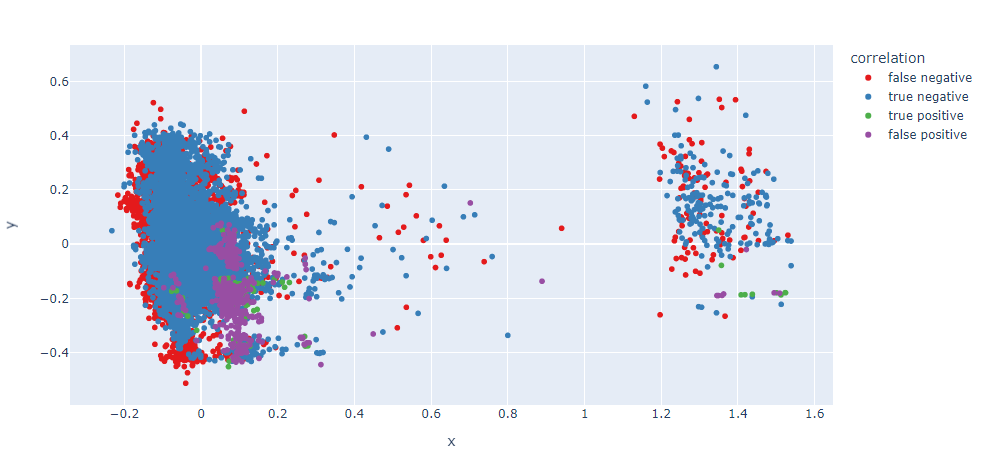
\includegraphics[width=14cm, scale=1]{images/worst_correlation_ssb1_quality_plot}
	\caption{Scatter Plot Correlazione Qualità Telemanom}
	\label{worst_clf_quality}
\end{figure}

La conferma arriva dalle matrici di confusione nelle Tabelle \ref{mvm-confusion1} e \ref{mvm-confusion2}. Sia KDE che Telemanom non riescono a trovare punti che siano effettivamente di qualità bassa. Per motivi di riservatezza vengono lasciati soltanto i valori percentuali e rimossi i conteggi.

Uno dei motivi per questi risultati poco incoraggianti deriva dal fatto che il numero di anomalie stimato tramite ${\gamma}GMM$ è troppo diverso rispetto al numero di punti considerati come anomali che hanno superato la soglia della banda A, abbassando di molto il numero di true-positive per tutti i modelli. Questo inoltre influenza i due modelli, KDE e Telemanom, che sono rispettivamente il migliore ed il peggiore, a produrre risultati simili.



\begin{table}[H]
	\begin{minipage}{.5\textwidth}
		\centering
		\resizebox{\columnwidth}{!}{%
			\begin{tabular}{|l|l|l|}
				\hline
				                  & \textbf{Real Positive} & \textbf{Real Negative} \\ \hline
				\textbf{Positive} &  0.05             &  0.05             \\ \hline
				\textbf{Negative} &  0.95            &  0.95            \\ \hline
			\end{tabular}
			}\captionof{table}{KDE Confusion Matrix}\label{mvm-confusion1}
	\end{minipage}
	\begin{minipage}{.5\textwidth}
		\centering
		\resizebox{\columnwidth}{!}{%
			\begin{tabular}{|l|l|l|}
				\hline
				                  & \textbf{Real Positive} & \textbf{Real Negative} \\ \hline
				\textbf{Positive} & 0.04             & 0.06             \\ \hline
				\textbf{Negative} & 0.96             & 0.94            \\ \hline
			\end{tabular}}\captionof{table}{Telemanom Confusion Matrix}\label{mvm-confusion2}
	\end{minipage}
\end{table}


\subsubsection{Confronto qualità - Alternative}
Si potrebbe tentare di risolvere i due problemi elencati ad inizio paragrafo andando a cambiare approccio per l'analisi della correlazione.
Per il primo di questi, ovvero il problema della media di tutte le registrazioni di qualità in un dato intervallo di 10 minuti che va a nascondere eventuali registrazioni più rare in cui la qualità è bassa, si può andare a contare il numero di registrazioni, sempre all'interno di ogni intervallo, che superano la soglia Q1 per la banda A.
I risultati ottenuti sono riportati nelle Tabelle \ref{count-sopra-soglia} e \ref{count-sopra-soglia-norm}. Per questioni di riservatezza, i valori sono stati alterati andando a moltiplicarli per uno scalare comune. 
Questa trasformazione non è un problema ai fini dell'analisi dei risultati in quanto i valori presi singolarmente non sono di particolare interesse, quello su cui ci si concentra è quanto differiscono i valori della colonna Intervalli Normali da quelli della colonna Intervalli Anomali.



Il numero medio di registrazioni che superano la soglia Q1 della banda A all'interno degli intervalli classificati come normali da KDE sono 27.56, valore persino più alto rispetto agli intervalli anomali. Questi risultati implicano che non c'è nessuna correlazione tra qualità bassa e punti anomali. 
Questo esperimento è stato fatto anche usando Telemanom ed anche qui i risultati confermano il trend.
La Tabella \ref{count-sopra-soglia-norm} mostra gli stessi conteggi ma rapportati rispetto al numero di registrazione per ogni intervallo. Può capitare che nel caso di problemi tecnici la frequenza di produzione si abbassi, andando quindi ad abbassare il numero di registrazioni MVM sopra-soglia. In questo caso calcolare la percentuale dei cuscinetti che superano la soglia rispetto al numero totale di cuscinetti registrati per intervallo può produrre risultati più corretti. 
Nonostante i risultati producano valori più alti, utilizzando KDE, per gli intervalli anomali, la differenza rimane ancora troppo esigua per confermare una qualche correlazione. 

\begin{table}[ht]
\centering
\resizebox{\textwidth}{!}{%
\begin{tabular}{|l|ll|ll|}
\hline
                & \multicolumn{2}{c|}{KDE}                                     & \multicolumn{2}{c|}{Telemanom}                               \\ \hline
                & \multicolumn{1}{l|}{Intervalli Normali} & Intervalli Anomali & \multicolumn{1}{l|}{Intervalli Normali} & Intervalli Anomali \\ \hline
Banda A         & \multicolumn{1}{l|}{27.56}              & 27.02               & \multicolumn{1}{l|}{28}                 & 16.8                 \\ \hline
Bande Combinate & \multicolumn{1}{l|}{121.54}              & 119                 & \multicolumn{1}{l|}{121.94}               & 108.55              \\ \hline
\end{tabular}%
}
\caption{\label{count-sopra-soglia}Numero medio di cuscinetti sopra-soglia per intervallo}
\end{table}

\begin{table}[ht]
\centering
\resizebox{\textwidth}{!}{%
\begin{tabular}{|l|ll|ll|}
\hline
                & \multicolumn{2}{c|}{KDE}                                     & \multicolumn{2}{c|}{Telemanom}                               \\ \hline
                & \multicolumn{1}{l|}{Intervalli Normali} & Intervalli Anomali & \multicolumn{1}{l|}{Intervalli Normali} & Intervalli Anomali \\ \hline
Banda A         & \multicolumn{1}{l|}{0.12}               & 0.12               & \multicolumn{1}{l|}{0.12}               & 0.08               \\ \hline
Bande Combinate & \multicolumn{1}{l|}{0.56}               & 0.57               & \multicolumn{1}{l|}{0.56}               & 0.50               \\ \hline
\end{tabular}%
}
\caption{\label{count-sopra-soglia-norm}Percentuale di cuscinetti sopra-soglia per intervallo}
\end{table}

Per quanto riguarda il secondo punto, ovvero il problema di considerare solamente un macchinario, si è pensato di andare a eseguire l'algoritmo KDE su tutti i macchinari di cui si hanno i dati della linea di produzione e aggregare insieme le etichette per ogni punto temporale.
Anche in questo esperimento i dati hanno bisogno di una fase di processamento aggiuntiva, ovvero è necessario allineare le registrazioni di tutti i macchinari tenendo in considerazione il tempo che impiega il cuscinetto a sfera a spostarsi lungo la linea di montaggio. In un esempio, ipotizzando tre macchine di cui la terza è MVM ed un cuscinetto a sfera che parte dalla linea di montaggio a tempo $t$, la prima macchina esegue la registrazione su quel cuscinetto a sfera a tempo $t$, la seconda a tempo $t+1$ e la terza a tempo $t+2$. Per allineare le registrazioni viene quindi rimossa un'unità temporale dalle registrazioni del secondo macchinario e 2 unità dalle registrazioni del terzo macchinario. Così facendo si crea un'istantanea delle registrazioni per ogni cuscinetto a sfera. Questo procedimento è simile a quello svolto per le valutazioni precedenti, con la differenza che in quel caso si aveva soltanto il macchinario M1 ed MVM, di conseguenza solamente i dati MVM erano da traslare.
Allineati i dati è necessario aggregare le etichette di ogni macchinario per ogni punto temporale. È stato scelto di applicare un approccio del tipo \textit{almeno uno}, ovvero se il modello di AD trova un'anomalia per un dato macchinario e per un dato punto temporale, quel punto temporale risulterà anomalo anche per tutti gli altri macchinari. 
Purtroppo però anche con questo approccio la corrispondenza tra anomalie e qualità è bassa, inoltre eseguendo l'algoritmo di AD su tutti e 10 i macchinari a disposizione e aggregando con il metodo \textit{almeno uno}, potenzialmente il numero di anomalie rilevate viene moltiplicato per 10, passando da un 5\% ad un 50\%. Questo fa lievitare i numeri di false positive a dismisura. Sia il plot scatter, Figura \ref{quality_all_machines} che la matrice di confusione, Tabella \ref{cm_quality_all}, sono stati posti per visualizzazione. Anche qui per motivi di riservatezza sono presenti soltanto i valori percentuali.

\begin{figure}[t]
	\centering
	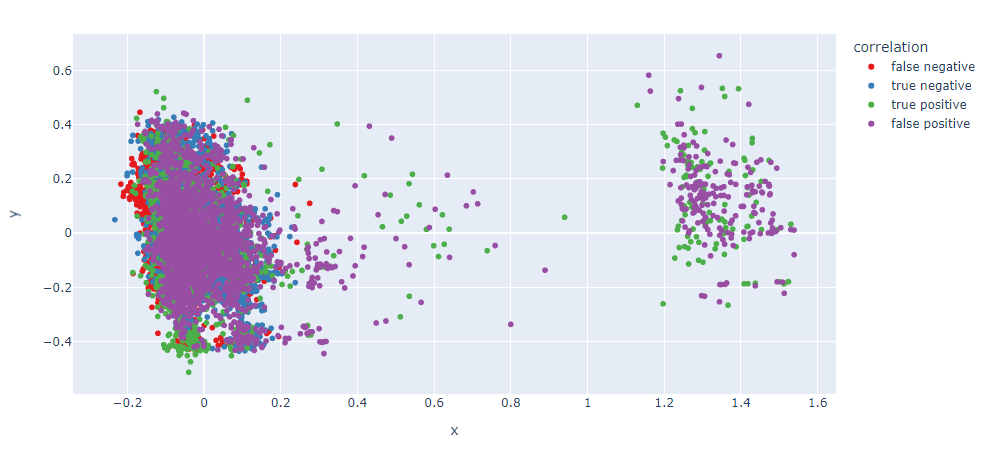
\includegraphics[width=14cm, scale=1]{images/correlation_all_quality_plot.png}
	\caption{Correlazione KDE su tutti i macchinari}
	\label{quality_all_machines}
\end{figure}

\begin{table}[]
	\centering
	\begin{tabular}{|l|l|l|}
		\hline
		                  & \textbf{Real Positive} & \textbf{Real Negative} \\ \hline
		\textbf{Positive} & 0.31            & 0.37            \\ \hline
		\textbf{Negative} & 0.69            & 0.63            \\ \hline
	\end{tabular}
	\caption{\label{cm_quality_all}Confusion Matrix KDE su tutti i macchinari}
	
\end{table}

\subsubsection{Conclusione}
In conclusione, valutare in modo automatico le performance di un modello di Anomaly Detection su SKF è molto difficile. Vista la complessità della linea di produzione, sarebbero necessari le registrazioni di almeno tutti i macchinari e frequenze di registrazione molto più alte. A questo punto un'analisi più accurata sulla relazione tra MVM e CoMo potrebbe essere svolta, ma anche in questo caso non è detto che ci sia correlazione perfetta.
Per ovviare a questa problematica si è deciso di portare in produzione una Dashboard con PowerBI, in modo da notificare gli operatori i momenti di anomalia e ricevere feedback di conseguenza sulla precisione del modello.
Una trattazione sul ciclo di distribuzione e di visualizzazione viene fatta nel capitolo successivo.
\clearemptydoublepage
\chapter{Deploy}

\begin{figure}[t]
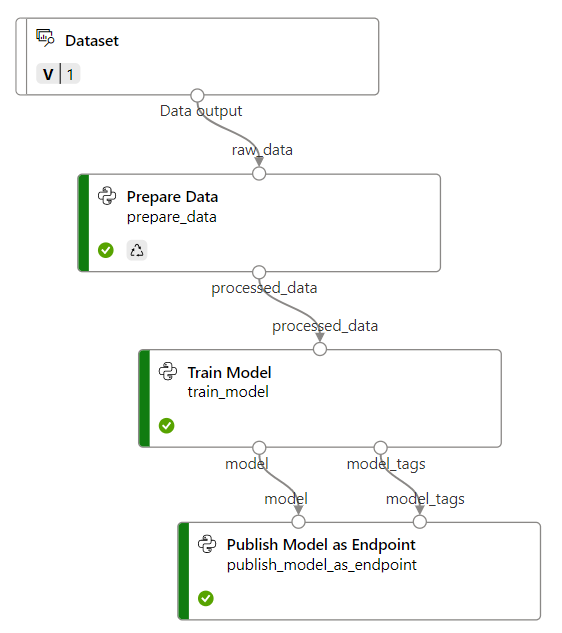
\includegraphics[width=10cm, scale=1]{images/pipeline}
\centering
\end{figure}

\begin{figure}[t]
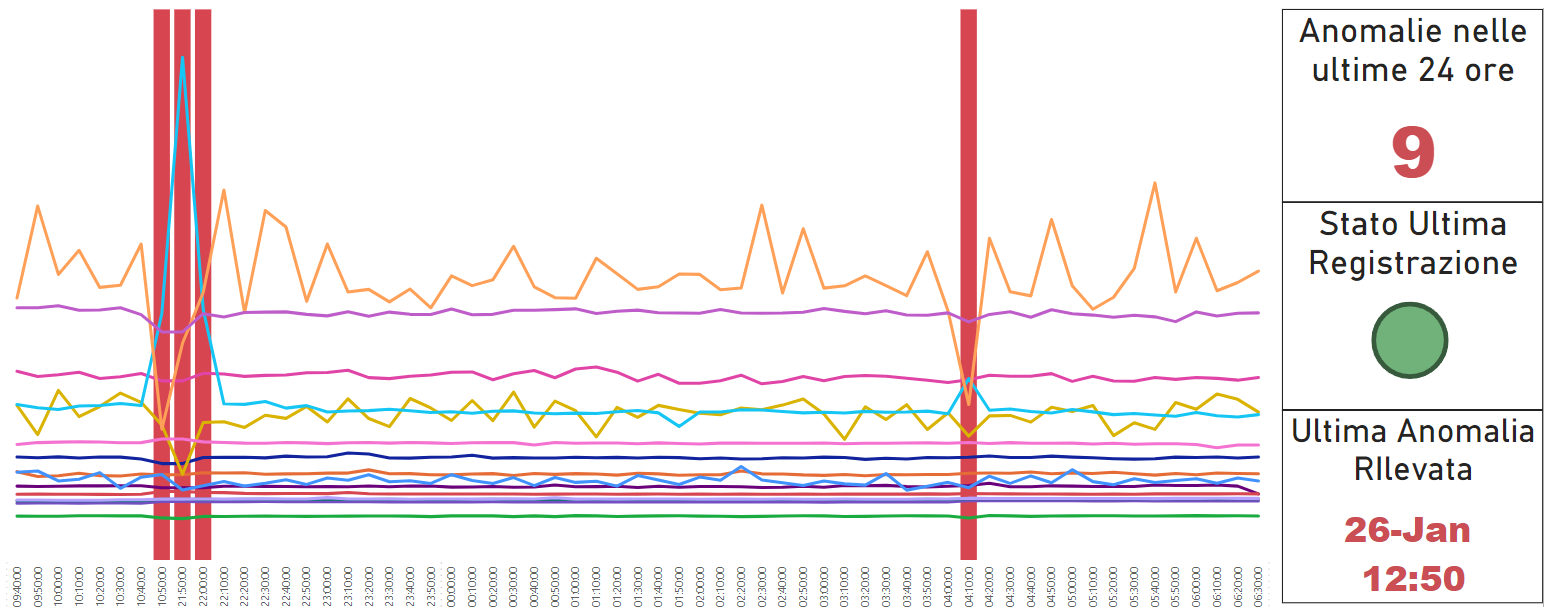
\includegraphics[width=14cm, scale=1]{images/powerbi}
\centering
\end{figure}

\clearemptydoublepage
\chapter{Conclusione}

%%%% TAIL OF THE DOCUMENT
\backmatter
%list of figures
\listoffigures
\clearemptydoublepage
%list of tables
\listoftables
\clearemptydoublepage
%bibliography
\addcontentsline{toc}{chapter}{Bibliography}
\bibliography{bibliography/bibThesis}
\bibliographystyle{ieeetr}
\clearemptydoublepage


\end{document}
